%\documentclass[a4paper,conference]{IEEEtran}
\documentclass[10pt,conference,letterpaper]{IEEEtran}
\usepackage{xspace}
\usepackage[dvipsnames]{color}
\newcommand{\tbd}[1]{XX-#1-XX}
\newcommand{\subparagraph}{}
\usepackage{graphicx}
\usepackage{amsmath}
\usepackage{array}
\usepackage{enumitem}
\usepackage{epsfig}
\usepackage{color}
\usepackage{subfigure} 
\usepackage{spverbatim}
\usepackage{gensymb}
\usepackage{algorithm,algorithmic}
\usepackage{amsmath}
\usepackage{amsfonts}
\usepackage{amssymb}
\usepackage{multirow}
\usepackage{etoolbox}

\newcommand{\wifi}{WiFi\xspace}
\newcommand{\christina}[1]{{\color{blue}[\textit{Christina: #1}]}} %Christina's comments
\newcommand{\mquote}[1]{``#1''} %Christina's quotes
\newcommand{\mallesh}[1]{{\color{green}[\textit{Mallesh: #1}]}} %Mallesh's comments

\makeatletter
\patchcmd{\@maketitle}
  {\addvspace{0.5\baselineskip}\egroup}
  {\addvspace{-1.0\baselineskip}\egroup}
  {}
  {}
\makeatother

\begin{document}
\title{ Scalable Ground-Truth Annotation for Video QoE Modeling in Enterprise WiFi}
\author{\IEEEauthorblockN{\#10 Pages, Paper ID \#18}
}

\maketitle
%!TEX root = ../main.tex
%\begin{abstract}

Applications for mobile Internet have proliferated with the increase in smartphone usage. Popular applications include Web browsing, video streaming and interactive telephony. A critical performance issue in these applications is quality of experience (QoE) of end-users. It is now widely understood that resource control mechanisms for such applications should optimize for QoE rather than more traditional quality of service (QoS) metrics that capture parameters such as latency or throughput.  The reason for this is that these QoS metrics do not always correlate well with the application-specific user experience or may have complex dependencies. In our work, we study the QoE aspects of three popular mobile applications -- YouTube for video streaming, Skype for telephony and Google Chrome for Web browsing. Our general goal is to aid resource control mechanisms to optimize for the QoE of applications. 
     
In the first part of our work, we conduct a survey of existing work on QoE optimizations and highlight their limitations. We then propose a machine learning-based QoE modeling approach. 
%This model is to be located at a WiFi access point or cellular base station. 
The model learns the QoE of applications under diverse network conditions and helps the network administrator to efficiently provision resources to maximize the QoE. The proposed approach improves the model accuracy significantly relative to prior approaches. 
      
In the second part of our work, we perform a detailed study on how underlying device hardware performance may impact the QoE of mobile applications when there are sufficient network resources available. For this study, we microbenchmark the applications with respect to device hardware parameters such as CPU clock speed, memory, GPU and number of CPU cores. We find that Web browsing is the most affected application when hardware resources are limited among the applications studied. The reason is that Web browsing is inefficient in exploiting any of the device accelerators or coprocessors. We show that offloading Web page load related computations opportunistically to the DSP coprocessor can lead to upto 18\% improvement in page load times while saving the energy consumption by a factor of 4.

%\end{abstract}

%!TEX root = ../paper.tex


\section{Impact of Device Performance} \label{intro}

\begin{figure*}[t]
    \begin{subfigure}[b]{0.33\textwidth}
        \centering
        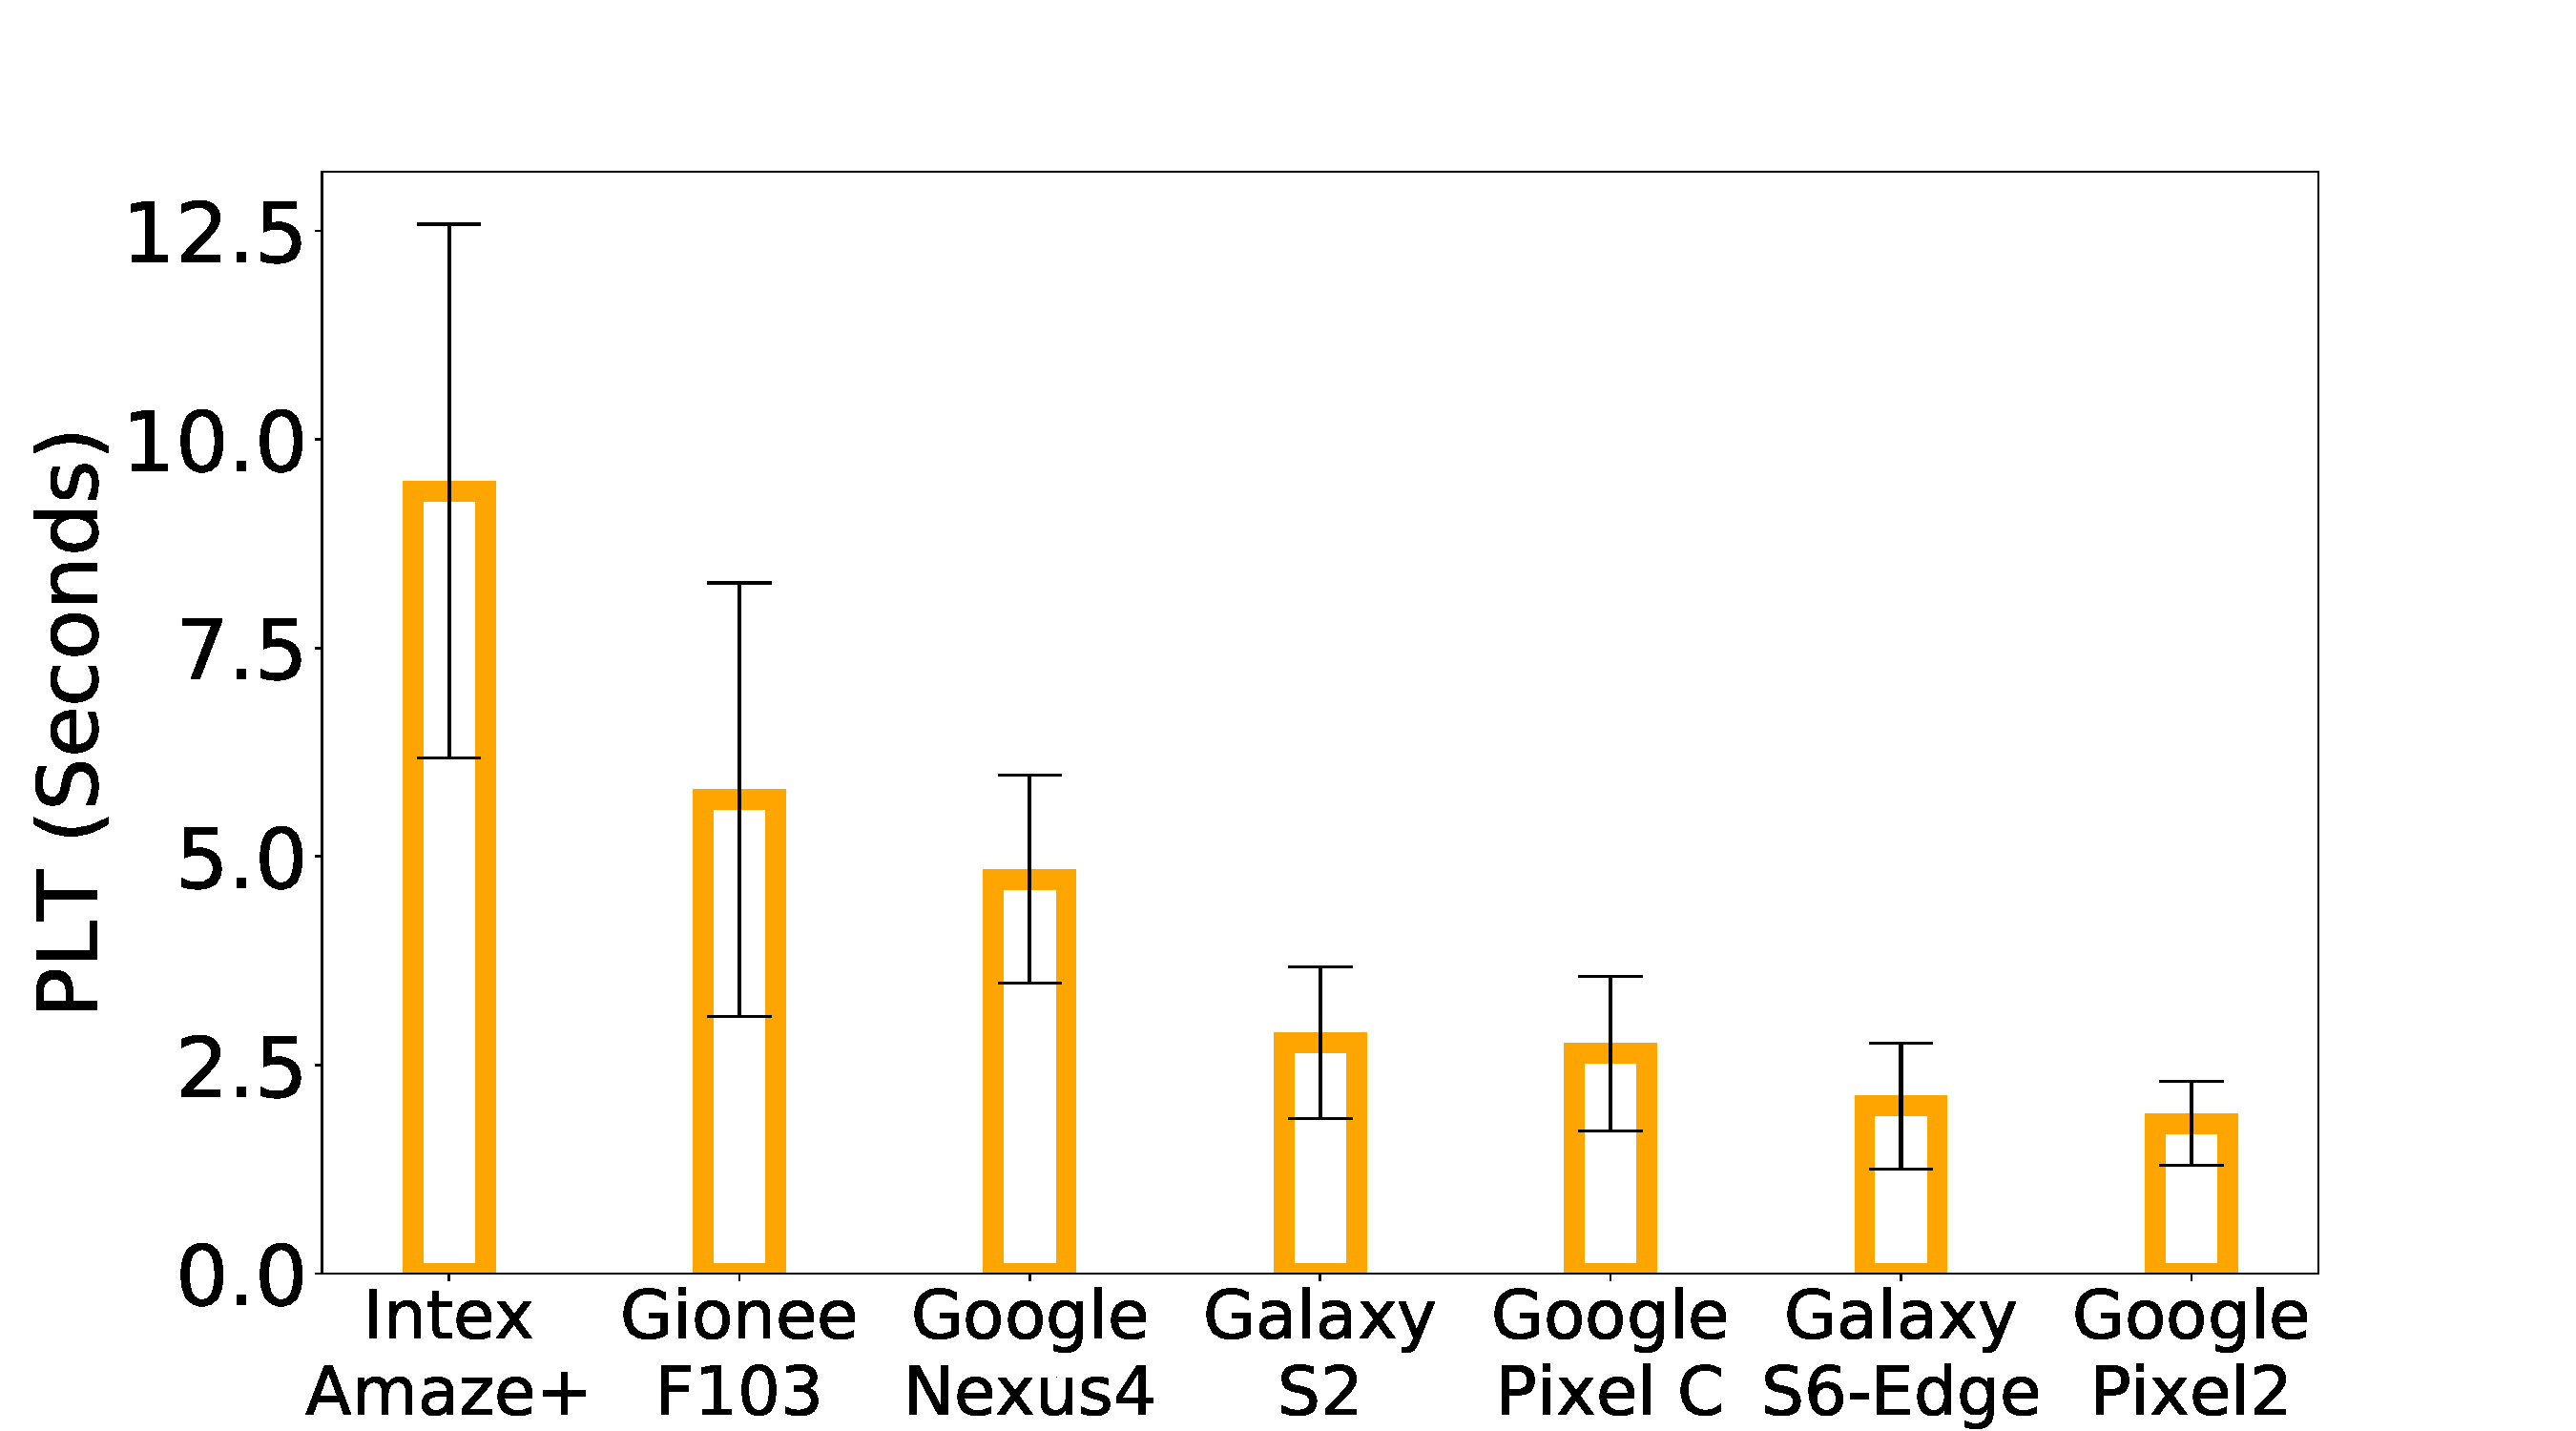
\includegraphics[width=1\linewidth]{sections/device-work/plt-devices}
        \caption{Web Browsing}
    \end{subfigure}
    \begin{subfigure}[b]{0.33\textwidth}
        \centering
        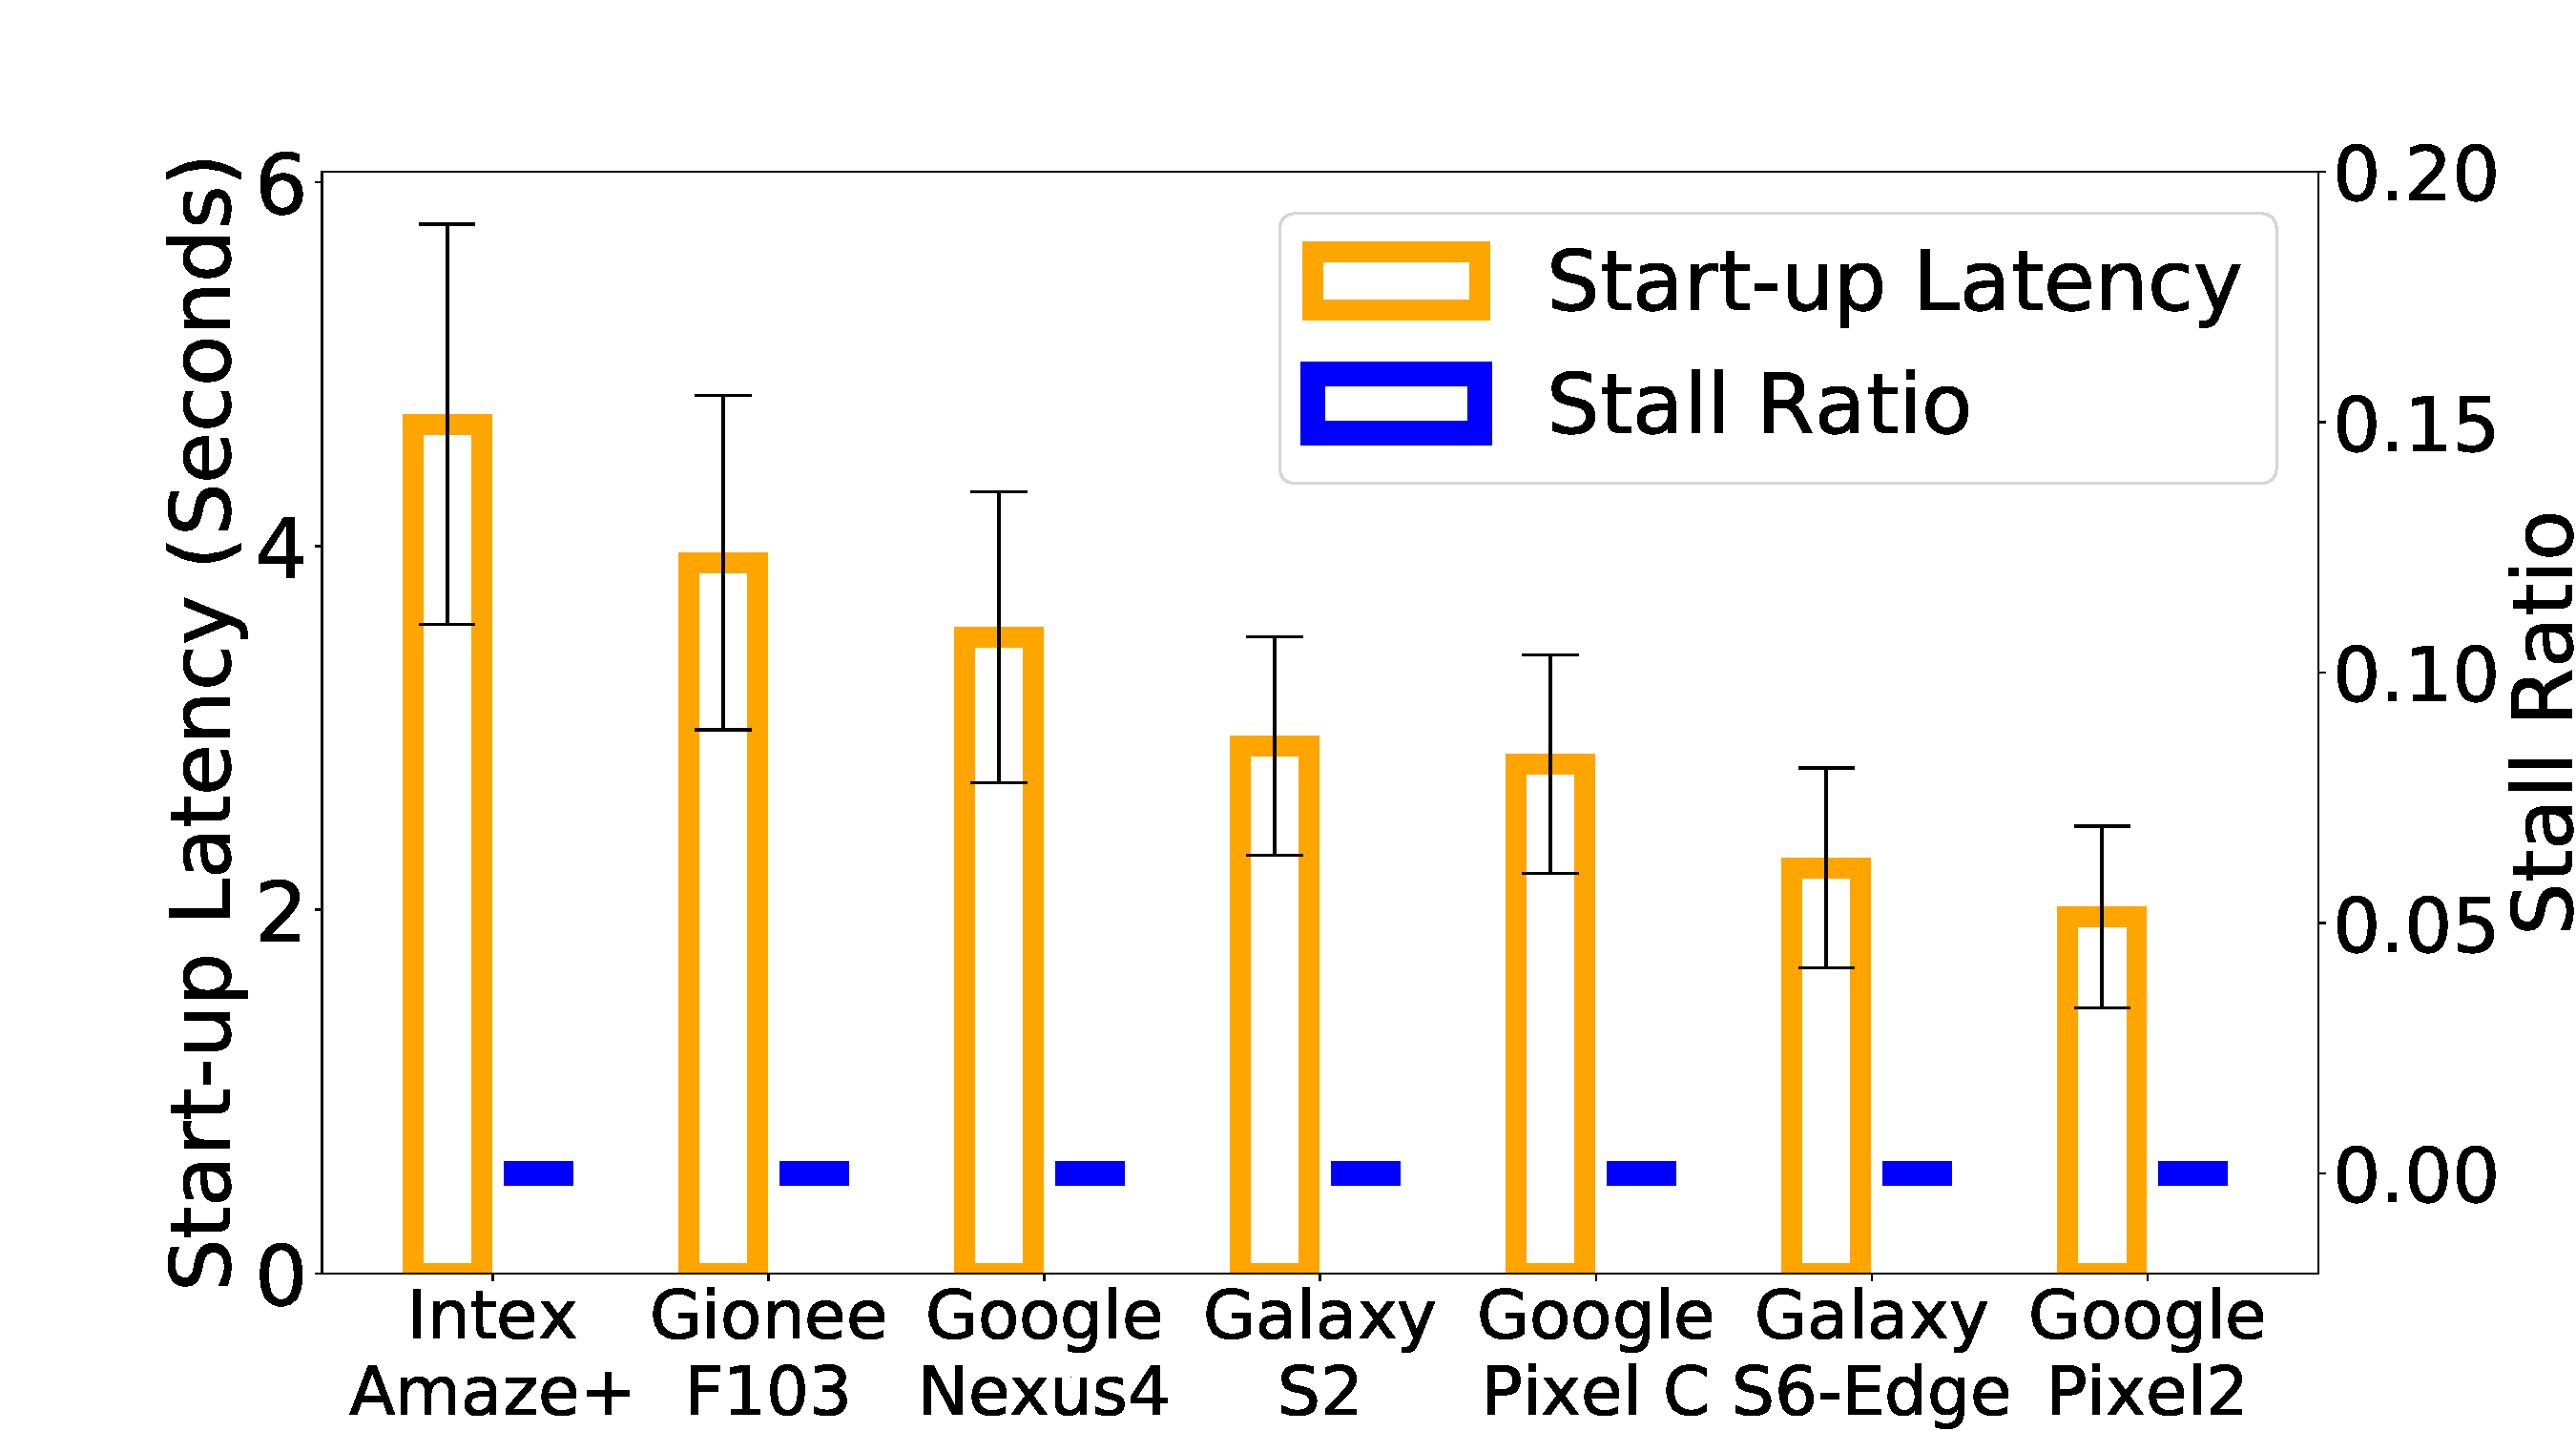
\includegraphics[width=1\linewidth]{sections/device-work/youtube-motivation}
        \caption{Video Streaming}
    \end{subfigure}%
    \begin{subfigure}[b]{0.33\textwidth}
        \centering
        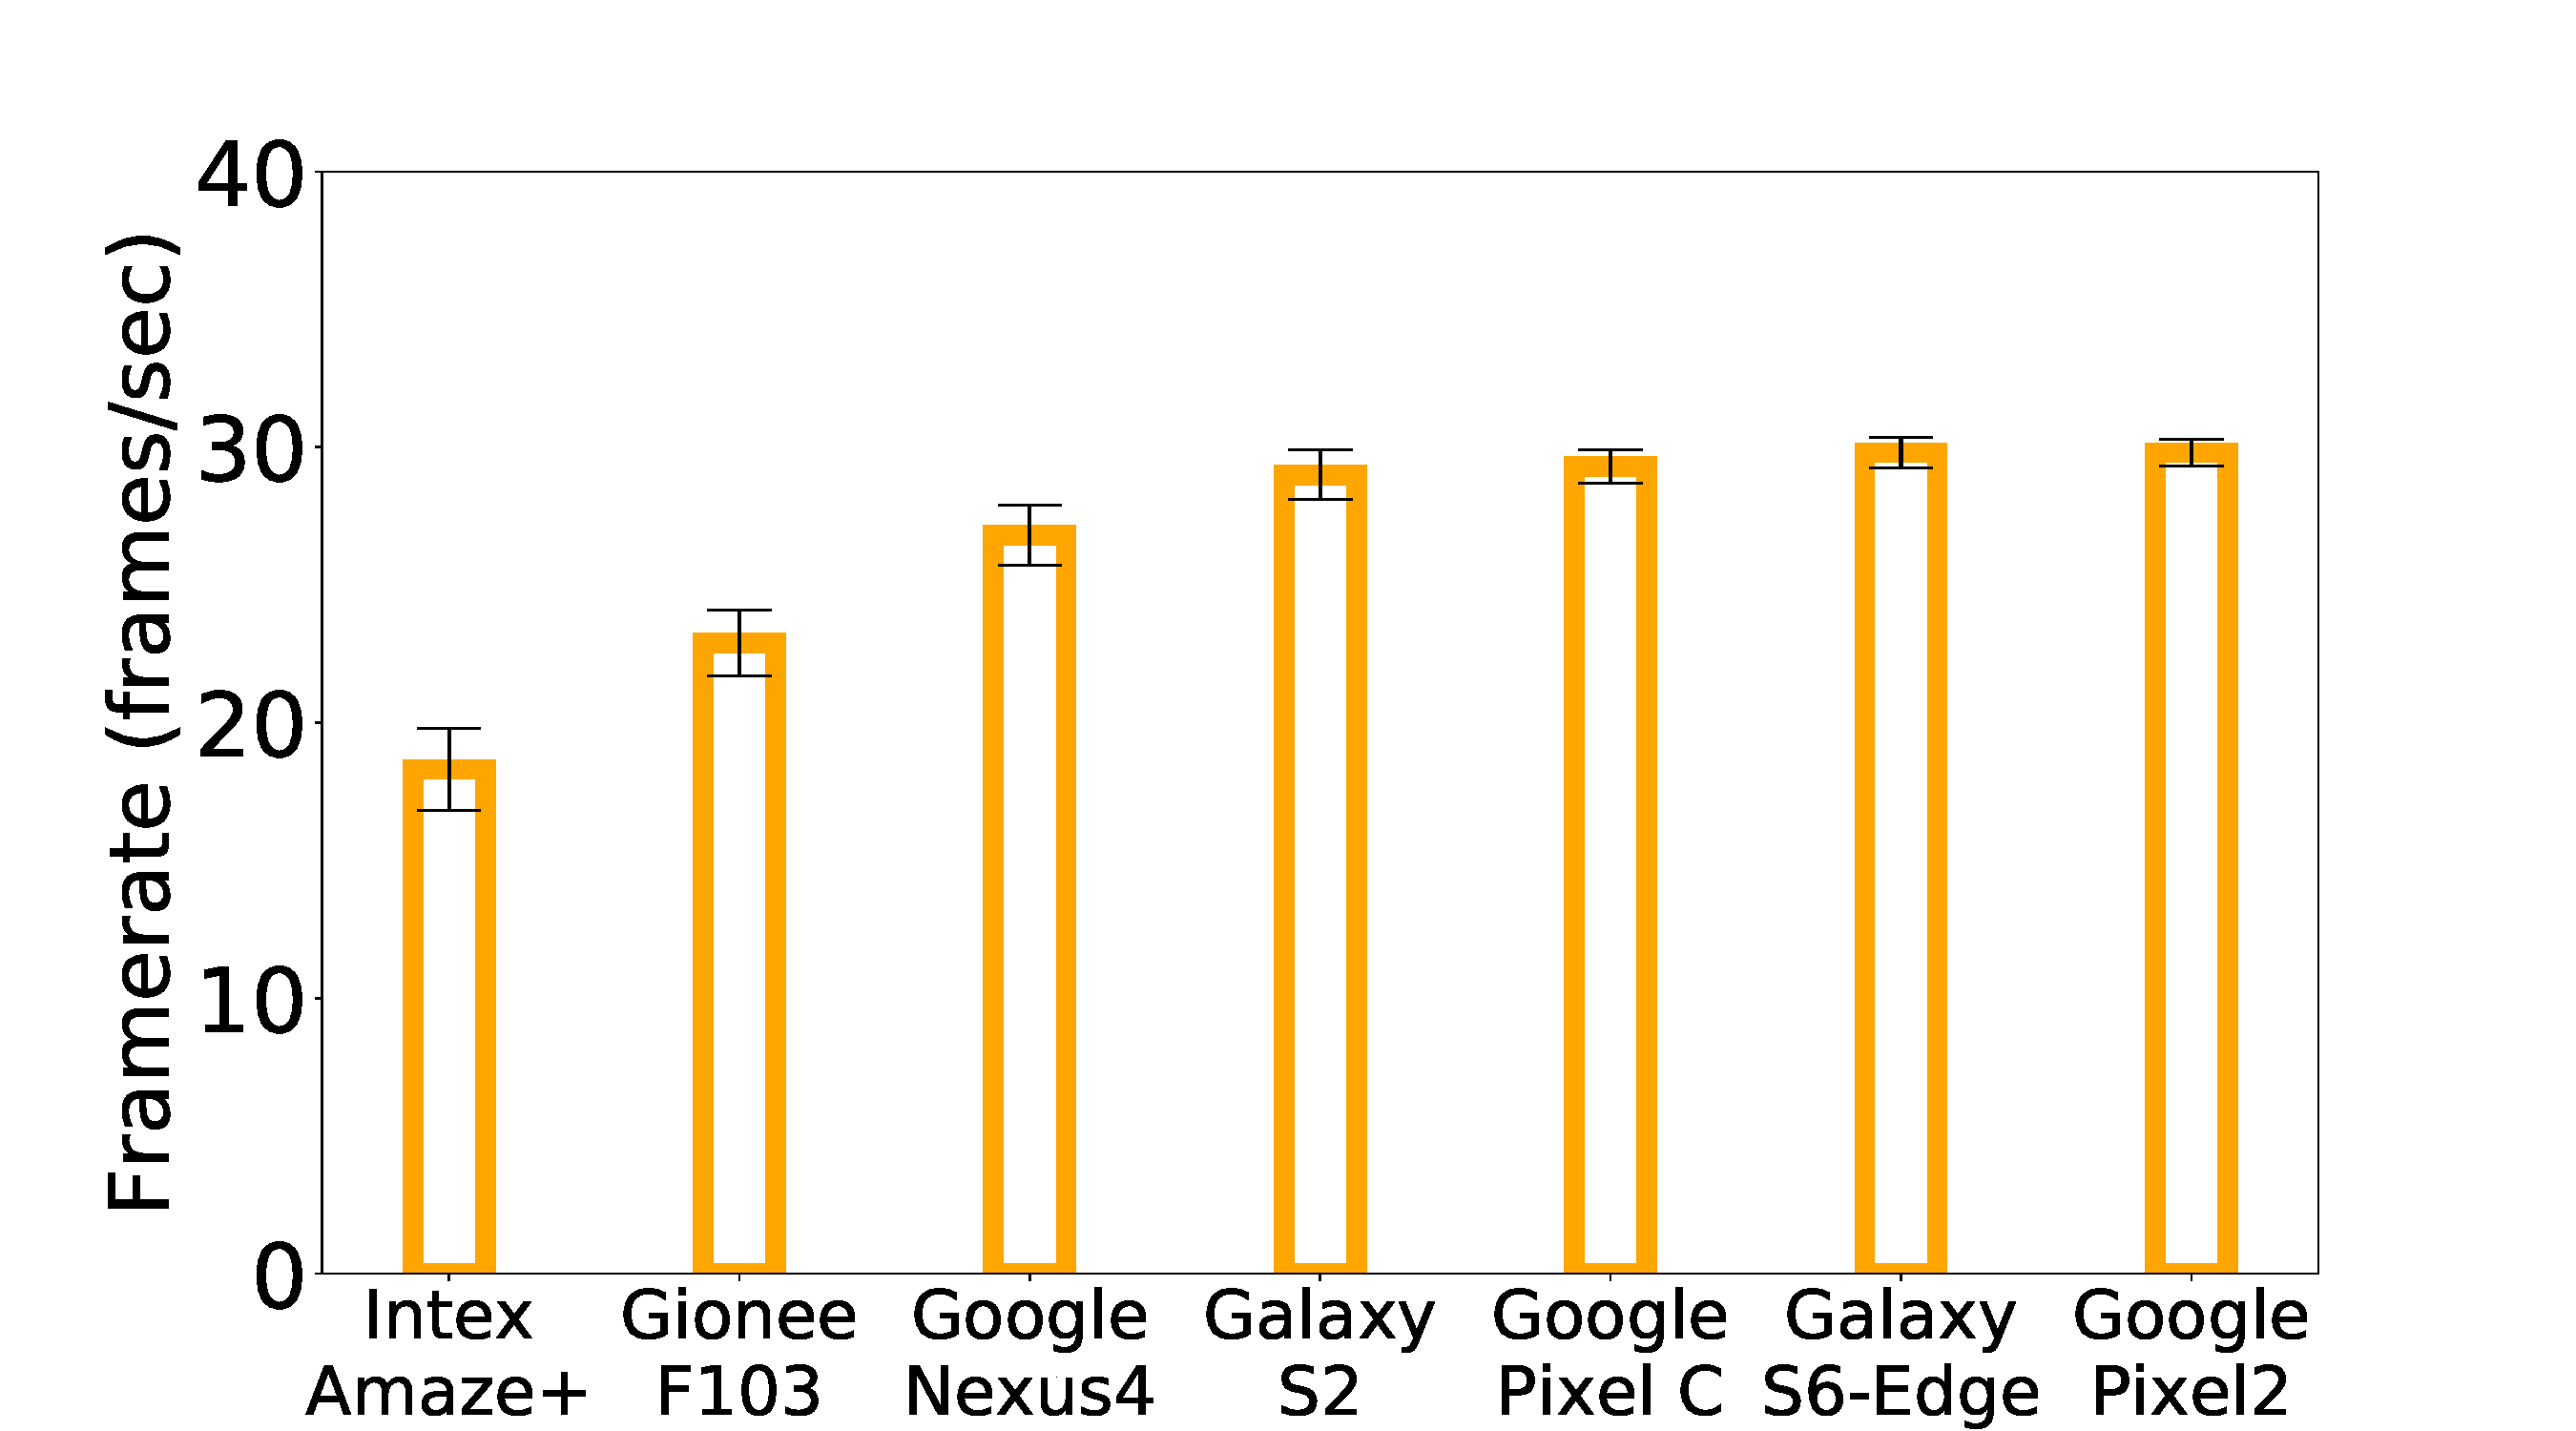
\includegraphics[width=1\linewidth]{sections/device-work/skype-motivation}
        \caption{Video Telephony}
    \end{subfigure}
     \caption{Mobile application performance across diverse devices: (a) Web Browsing, (b)Video Streaming, (c) Video Telephony. The horizontal axis shows the device type; their corresponding specifications are tabulated in Table~\ref{tab:device_types}.}
     \label{fig:motivation}
\end{figure*}

\begin{table*}[t]
  \centering
   \scalebox{0.9}{
  \begin{tabular}{c|c|c|c|c|c|c|c}
  \hline \hline
    \textbf{Device} & \textbf{Application} & \textbf{Number} & \textbf{OS} & \textbf{Clock} & \textbf{GPU} & \textbf{RAM} & \textbf{Release} \\
      \textbf{Name} & \textbf{Processor} & \textbf{of Cores} & \textbf{Version} & \textbf{Min-Max (Mhz)}  & \textbf{Type} & \textbf{Size (GB)} & \textbf{Cost} \\
    \hline
    \hline
    Intex Amaze+ &Spreadtrum SC9832A&4&6.0&300-1300 &Mali-400&1&\$60\\
    Gionee F103 &MediaTek MT6735&4&5.0&300-1300 &Mali-T720&2&\$150\\
    Nexus4 &Snapdragon S4 Pro&4&5.1.1&384-1512 &Adreno 320&2&\$200\\
    SG S2-Tab &Exynos 5433&8&5.0.2&400-1300 &Mali-T760&3&\$450\\ 
    Pixel-Tab &Tegra X1&4&8.0.0&204-1912& Maxwell&3&\$600\\ 
    SG S6-edge &Exynos 7420&8&6.0.1&400-2100 &Mali-T760&3&\$880\\
    Pixel2 &Snapdragon 835&8&8.0.0&300-2457 &Adreno 540&4&\$700\\ \hline \hline
  \end{tabular}
    }
  \caption{The table shows the set of diverse mobile devices used in our motivation experiment and their corresponding specifications including cost, CPU capabilities, and memory capacity. }%Mobile Devices in our Experiments showing OS/Hardware Specifications: Shown are parameters that impact the performance of mobile applications}
  \label{tab:device_types}
\end{table*}
While mobile smartphones have now penetrated 
a significant fraction of world population, the devices 
vary widely in terms of cost and performance. 
For example, the smartphones in the market 
range from $\approx$\$50 to $\approx$\$1000~\cite{mobilephones, contreras2017patents}, and the cost 
largely depends on the hardware specifications. 
For example, a \$600 phone such as OnePlus5 has 8 cores, running upto 2.4\,Ghz clock and 6\,GB RAM, while a cheaper \$60 phone (e.g., Dell Venue Pro) only has 2 cores with up to 1\,GHz clock and 512\,MB RAM. 

However, the impact of the hardware specs
on the performance of mobile Internet applications is not well-studied. A large fraction of past research on mobile Internet performance has focused on the effect of the {\em network} on the applications~\cite{butkiewicz2015klotski, kelton2017improving, singh2015flexiweb, Ruamviboonsuk:2017:VAM:3098822.3098851, Shafiqund, Xiaodash2m, chen2016effective} but not 
the device. Some studies do address the compute performance of mobile Internet applications~\cite{zhu2017optimizing,jones2009parallelizing,mai2012case}, but the underlying
technologies developed are more suited for higher end devices. 

Given that a large fraction of mobile
users in developing regions (62\%-68\% by some 
account \cite{unity}) uses smartphones with relatively
less expensive lower end hardware, it is important
to understand the impact of the device hardware on the 
performance of the mobile apps. In fact, with the increased 4G penetration, network speed is no longer the bottleneck in many developing countries~\cite{mobilephones,contreras2017patents,jioplans1,jioplans2}.  Our measurements show that mobile Web page loads on two popular phones in India, Intex Amaze 4 ($\approx$\$60) and Gionee ($\approx$\$150) are $5\times$ to $3\times$ worse, respectively, compared to Web page loads on Google Pixel2 ($\approx$\$700) under the same network conditions (\S\ref{sec:motivation}). 
This underscores the importance of studying the influence of the device hardware
on the performance and explore ways to improve the mobile web experience on lower end hardware. 

In this paper, we focus on three types of mobile Internet applications:  {\em (i)} Web browsing, {\em (ii)} video streaming, and {\em (iii)} video telephony. We study performance in terms of Quality of Experience (QoE) and energy. We especially focus on how the {\em CPU clock frequency} impacts performance 
given that the clock frequency
has the most impact on the performance
among other aspects of the specification (\S\ref{sec:impact_cpu}).% varies  important resource that changes across low-end and high-end devices as the representative   
%However, our experiments show that the CPU clock has the most impact on application performance among these resources (\S\ref{sec:impact_cpu}). 
%For example, \todo{write something here to convince that this is the case}.
%\mallesh{We show this by measuring Web performance under different clock, memory and GPU conditions on Nexus4 phone. We find a low memory of 512MB RAM has an impact of 4 seconds increase in PLT while a lower clock of 384Mhz shows 11 seconds increase in PLT. We also measure the impact of disabling GPU, which has a 0.5 seconds difference from normal PLT which is 3.5 seconds. This shows that Clock frequency has an exponential increase in PLT.}
%The second problem that we solve is curating different hardware conditions. It is difficult to measure the application performance on various smartphones available in the market. So we take the approach of emulating these diverse smartphones by using a representative hardware parameter of smartphones. In our research, we find clock frequency of CPU is a key factor in application performance. Clock frequency directly determines the amount time required for certain computation. Hence, we use clock frequency parameter to emulate different smartphones because we find smartphones with clock frequency ranging from 300Mhz to 2.4Ghz in the market. We change the clock frequency with the help of clock frequency scaling algorithm called governor (Userspace) provided by Andriod. This allows us to fix the CPU clock on a smartphone.
%The QoE of an Internet application depends on several factors apart from the device hardware, including the network condition, the server, and other factors in the data delivery path. The problem is these factors are interdependent on one another (for example, impact of hardware on network apart from application computation). 

One of our key findings is that a slow CPU speeds not only affects compute performance, but has a second-order effect on the network
performance. In our measurements, for example, the TCP performance drops more than 20\,Mbps, 
when the CPU clock of the phone drops from 1512\,Mhz to 384\,Mhz. This is owing to 
the fact that a slower clock
increases TCP processing delays by as much 
as $\approx$12\,ms.
%In our experiments, the time between when the packet reached the kernel to when it reached the application differs by as much as 11ms between a slow and a fast CPU. 
The implication is that the application is doubly 
impacted by the slower clock that slows
down both the network latency/throughput as well as the compute 
performance inside the application. 
%since Internet application performance depends on both the network and the compute performance. 
% to low clock frequencies---affecting both compute and network. Application performance is a combination of the network performance, involving loading network objects, and computation performance, involving processing. 

Our goal now is in {\em isolating} the effect of CPU clock on the network and the compute activities of the application. This isolation is critical to shed light on how the application 
performance can be improved for low-end devices: should the optimization focus on improving the TCP packet processing or the application compute? While straightforward for video applications, for Web browsing, this isolation is challenging.  
Loading of Web objects, a network process, and processing of these objects, a compute process, are intertwined during the page load process and cannot be cleanly separated. To this end, we leverage the WProf tool~\cite{wang2013demystifying,nejati2016depth} that breaks down the Web page load process into network and compute processes on the critical path. The key findings of our study are: %In the case of video applications, we isolate the effect of network and compute by

\begin{itemize}    

   \item {\bf Mobile Web performance is significantly affected by slow clocks:} Web page loads slow down by a
    factor of 5 on average when CPU clock speed reduces from 1512 Mhz to 384 Mhz. This slow down is both because of compute processing delays and the second-order effect in network processing. Our isolation experiments show that compute processing is more of a bottleneck under slow CPU speeds, accounting for over 60\% of the 
    page load time. Within the compute activities, Javascript evaluation is affected most by 
    the CPU slow down, and rendering and painting are affected the least.
 
 %  the web page load slowed down by an average of 6 times across XXX Web pages, even when the network condition is held a constant. Under slow CPU clock, the processing of the Web objects slowed down, but the network loading is also affected because of the second-order effect described earlier. Using our isolation technique, we find that compute accounts for XXX of the slow down under low clocks. This result suggests that improving Web performance for low-end phones should focus on improving the performance of compute. 
   
   %The Web page load process consists of both network activities for loading objects, and compute activities for parsing HTML, running scripts, and rendering. Reducing CPU speeds both affects the compute activities directly, and the network downloads through the second order effect described earlier. To isolate this, we build an emulator which schedules object downloads by keeping the compute the constant. While scheduling object downloads, we preserve the dependencies captured using WProf tool. 

    \item {\bf A slow clock does not significantly affect video streaming because of offloading and pre-fetching:} 
    The QoE of video streaming is largely unaffected by slow CPU speeds, despite video streaming being a compute-intensive application. By isolating the impact of compute and network, we find that this paradox is because of two reasons. From the compute standpoint, 
     streaming applications use special hardware decoders, even available on low-end phones, to process video data rather than decode on the CPU.   %(e.g, \texttt{OMX.sprd.h264.decoder}). 
    From the networking standpoint, streaming applications pre-fetch enough data and are unaffected by the second-order network slow-downs caused by slow CPU. 
    
 %\item {\bf  Increasing CPU speeds beyond a inflection point has poor performance/power trade-off:} For all three applications, increasing  CPU speeds significantly increases energy consumption. However, the corresponding improvement in performance beyond a point is not commensurate with the energy cost. 

 \item {\bf Leveraging hardware offloading is a promising approach to improve Web performance under slow clock:}  Similar to the hardware offloading techniques used in video applications, offloading Javascript to a low-power DSP can potentially improve Web performance. Our preliminary 
 analysis with offloading only regular expression evaluations
shows that the improvement can be as much as 18\% in page load time along with a $4\times$ 
improvement in power consumption. %\todo{check the numbers.} 
\end{itemize}



\subsection{Motivation for Scalable QoE Annotation} \label{MOTIVATION}

In this section, we describe the need for new QoE metrics for enterprise networks and the limitations of existing work. 

\noindent {\bf Lack of QoE information from applications}:
While several works have motivated and addressed the problem of network-based QoE estimation~\cite{aggarwal2014prometheus}, little attention has been paid to the problem of collecting the QoE ground-truth. Most works have relied on application-specific information. This approach is effective for QoE optimizations by content providers, as they only focus on a single application~\cite{balachandran2013developing} or initial training of QoS to QoE model~\cite{aggarwal2014prometheus}. Nevertheless, administrators of access networks have to ensure good experience for a wide range of diverse applications being simultaneously used. 
Table~\ref{tab:table1} shows that not all popular video applications provide QoE information. 
Even for applications like Skype, availability of technical information depends on the version of the application and on the OS (e.g., no technical information for iOS). 

To apply QoE estimation models in real networks, we need to remove the dependency of QoE metrics on application features, such as Skype technical information. One way to achieve this is to simply record the video as it plays on the mobile device and analyze this video for quality. 

\noindent {\bf Lack of scalable and reliable  QoE measures:}
Prior work on video quality evaluation leverages \emph{subjective and/or objective} metrics. 
Subjective metrics are measured with MOS collected through user surveys. 
They capture absolute QoE but are tedious to conduct and to scale. 
QoE metrics need to scale to thousands of videos in order to train models that map QoS to QoE. 
Alternatively, objective metrics can be computed from the video. 
Objective metrics are further classified in two categories: reference and no-reference based. 
A reference-based metric uses both sent and received video, and compares the quality of sent vs.~received frames. 
As it is challenging to retrieve and synchronize reference videos for telephony applications, no-reference based quality metrics are preferred. 
Jana {\em et al}~\cite{jana2016qoe} have proposed a no-reference metric for QoE estimation in Skype and Vtok. 
They record received videos for each of these mobile telephony applications and compute three no-reference metrics: {\em blocking, blurring} and {\em temporal variations}. 
Then, they combine these three metrics into one QoE metric by using MOS from subjective user study. 
Their study shows that blocking does not impact MOS of a video clip. 
While they show that their {\em blur} and {\em temporal variation} metrics correlate well with MOS, they do not evaluate these metrics over a wide range of clips. 
%For example, one can wonder if {\em blur} is sensitive to the video content. 

We conduct similar experiments with Skype to evaluate blur metric of prior works. 
Our experimental setup is described in Section~\ref{label:design}. 
To capture video blur, Jana {\em et al}~\cite{jana2016qoe}  employ discrete cosine transform (DCT) coefficients \cite{marichal1999blur} from the compressed data by computing the histogram of DCT coefficients thereby characterizing the image quality. 
The DCT coefficients are obtained in transform coding of video compression process, as described in Section \ref{label:background}. 
The assumption here is that blurred image has high-frequency coefficients close to zero. 
Hence, the method studies the distribution of zero coefficients instead of absolute pixel values. 
Although the method estimates out-of-focus blur accurately, it falls short in estimating realistic blur and sensitivity to noise. 
The authors also point out that the method is very sensitive to uniform background and images with high luminance components. 
In Fig. \ref{fig:ucdavis}, we evaluate blur for 20 video sequences\footnote{\scriptsize{The videos are located at \textit{https://gofile.io/?c=iyfQND}.}} using DCT metric. 
We have collected these videos in a representative manner to cover diverse content, different types of motion and we have downloaded them in Full HD resolution. 
The same 20 videos are converted to low quality by compressing and decreasing the resolution, to observe the difference of DCT metric between high and low quality videos.

\begin{figure}[t]
	\centering
	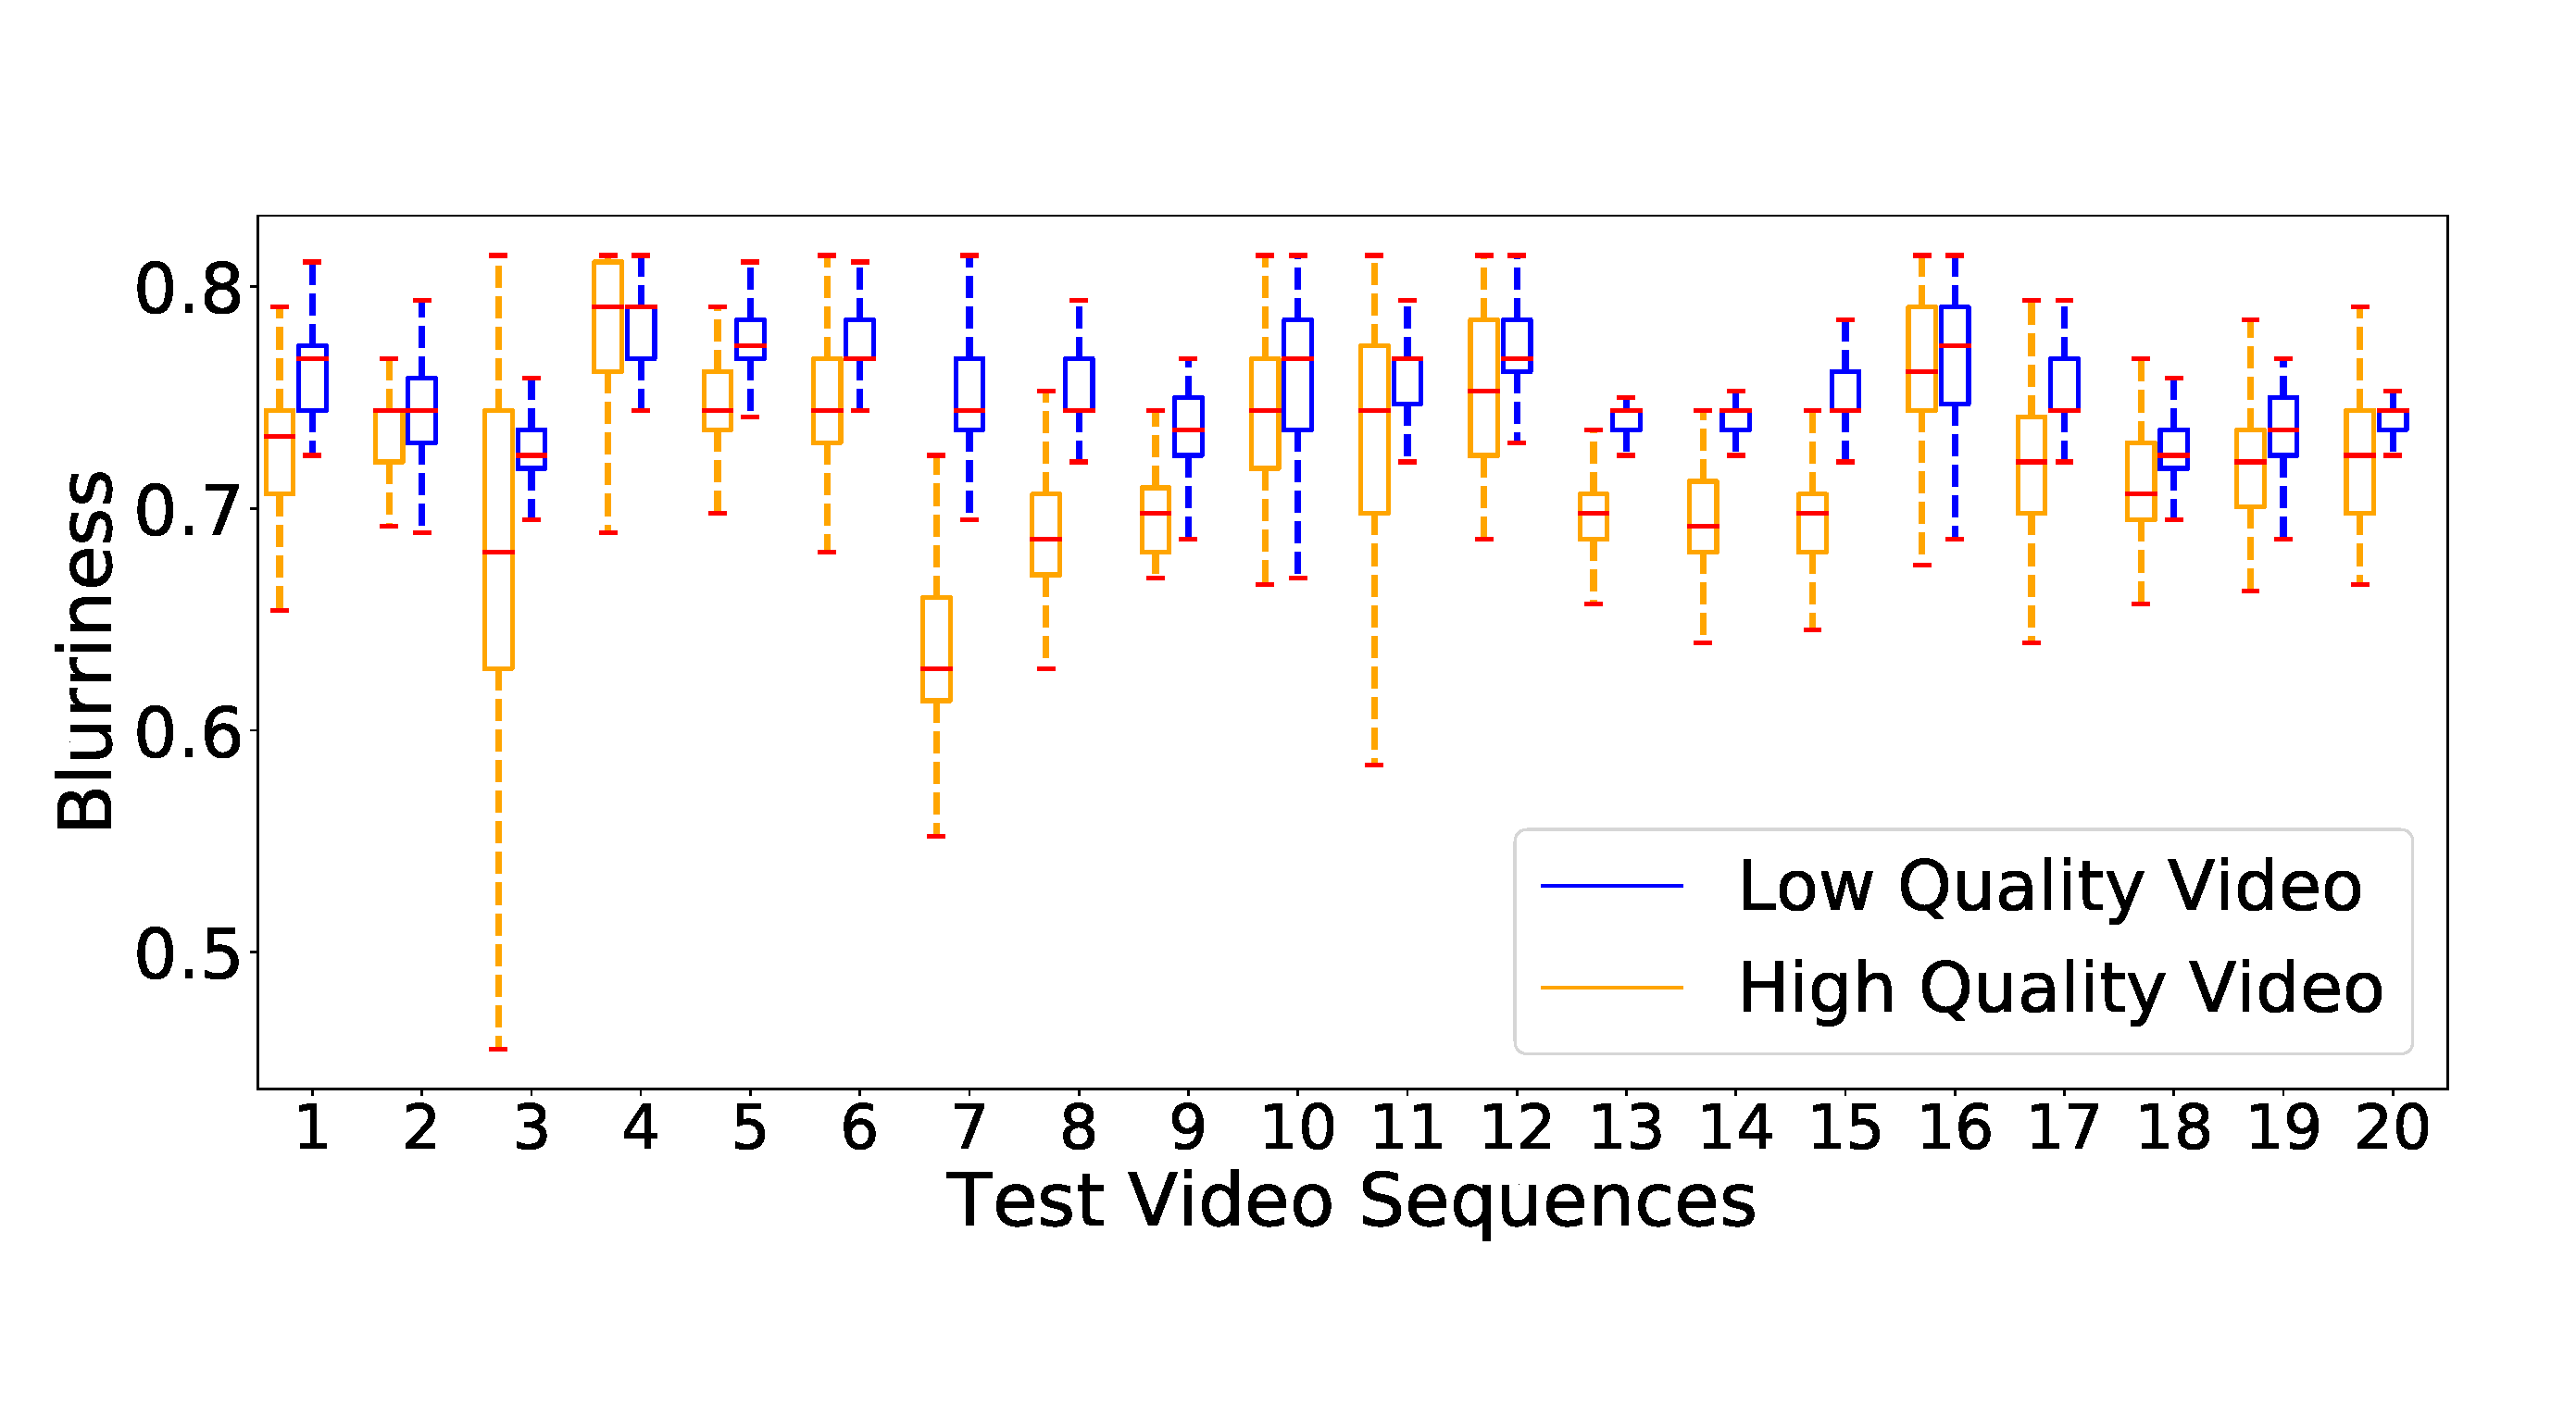
\includegraphics[width=\linewidth]{sections/network-work/dct-blur}
	\caption{Blur detection using DCT coefficients~\cite{jana2016qoe,marichal1999blur}. DCT coefficients fail to distinguish between high and low quality video due to content diversity.}
	\label{fig:ucdavis}
\end{figure}

We notice two aberrations of the DCT metric by Jana {\em et al}~\cite{jana2016qoe}: First, the metric is indeed content-specific i.e., although it produces high blur values for some low quality videos, it also shows high blur values for some high quality videos. For instance, videos 2 and 4 contain mostly over-illuminated and dark images and are equally tagged as blurred in both low and high quality scenarios. Second, DCT metric fails to detect accurate blur levels, even if the image is blurred heavily i.e., it shows low blur differences ($<$0.2 blurriness) between high and low quality videos even though we created extremely low-quality videos (240p resolution and high ($>$200\%) compression). Even for a single video, this DCT metric shows a lot of variation, such as for videos 3 and 11, raising concerns about its accuracy. We evaluate the accuracy of this blurriness metric in Section \ref{label:model}, showing a MOS error larger than 1.2. We also experiment with four other well-known blur metrics \cite{golestaneh2014no, mittal2012no, tong2004blur, marziliano2002no}, but none of these methods are consistent across diverse videos. This challenges the scalability and versatility of this blur metric in the wild. 

The {\em temporal variation} metric proposed by Jana {\em et al}~\cite{jana2016qoe} aims to capture video stalls and considers the ratio of missed frames to total number of frames in a video, but the metric requires the number of frames sent over the network. We need the reference video to compute the total number of frames in the video, thus the metric is not entirely no-reference. 
In enterprise networks, a QoE metric needs to be applicable to diverse contents and to not rely on access to reference video.
Further, there are many other previous works \cite{wolf2009no, borer2010model, usman2017no, pastrana2006automatic} focused on measuring the temporal jerkiness. We find these methods  either are parametrized or are sensitive to resolution and to frame rate of the video or are unable to scale across diverse video contents. The above limitations motivate us to propose new metrics that can accurately measure blurriness and freezes across diverse video content.

{\bf Need for a model per application category:}
When analyzing a recorded video for an application, the QoE metric has to be sensitive to the application category as different applications have to meet diverse performance guarantees. For instance, streaming quality is impacted largely by buffering and stall ratio, whereas telephony quality is impacted by bit rate, frames per second, blocking and blurring in the video. Table~\ref{tab:qoe_metric} lists examples of QoE metrics corresponding to different applications. Therefore, one needs to capture different artefacts when designing models for multiple application categories.

To address the aforementioned requirements, we seek to answer the question: {\em How to scalably label the quality of a video call, without any support from the application?}

\begin{table}[t]
	\centering
		%\scriptsize
            %\resizebox{\columnwidth}{!}{
			\begin{tabular}{l|c}
				\hline \hline
				\textbf{Application} & \textbf{Ground-truth} \\
				\hline
				\hline
				Skype & \checkmark *on some versions \\  \hline
				Hangouts/Duo & $\times$ \\ \hline
				FaceTime & $\times$ \\ \hline
				YouTube/Netflix & \checkmark \\ \hline 
			\end{tabular} 
		%}
        %\vspace*{0.2em}
		\hfill 
		\caption{Availability of QoE ground-truth}
		\label{tab:table1} 
        	%\vspace*{-2em}	
%	}
\end{table}

\subsection{Background} \label{label:background}

Before designing our no-reference QoE metrics, we present a video coding primer and QoE artefacts in video telephony.
In Section~\ref{label:design}, we harness these coding properties to carefully craft accurate metrics that capture such artefacts.

\subsubsection{Video Coding Primer}
Video coding is performed in three critical steps: 

\begin{itemize}[leftmargin=*]
\item \textbf{Frame prediction:}
    The encoder takes images of video and divides each image into macroblocks (typically 16x16, 16x8, 8x16, 8x8, 4x4 pixel blocks). The macroblocks are predicted from previously encoded macroblocks, either from current image (called \emph{intra-frame prediction}) or from previous frames and future frames (called \emph{inter-frame prediction}). Depending on the intra- and inter-macroblocks, frames are classified as I, P and B frames. The I frame uses only intra-frame prediction i.e., it does not employ any previously coded frames as reference. Whereas P frames are predicted using previously coded frames and B frames are encoded from previous and future frames. The encoder typically combines both intra- and inter-prediction techniques to exploit spatial and temporal redundancy, respectively. Intra-frame prediction involves different prediction modes \cite{richardson2004h} while finding candidate macroblocks. Inter-frame prediction uses motion estimation by employing different block matching algorithms (such as Hexagon based or full exhaustive search) to identify the candidate macroblock across frames. Finally, a residual is calculated by taking the difference (measured typically using mean absolute difference (MAD) or mean squared error (MSE)) between the predicted and current macroblock. The prediction stage produces 4x4 to 16x16 blocks of absolute-pixel or residual values. 

\item \textbf{Transform coding and quantization:}
These absolute values are then transformed and quantized for further compression. Typically, two transform coding techniques (block or wavelet based) are used to convert pixel values into transform coefficients. A subset of these transform coefficients are sufficient to construct actual pixel values, which means reduced data upon quantization. The most popular transform coding is DCT over 8x8 macroblocks. 

\item \textbf{Entropy coding:}
Finally, coefficients are converted to binary data which is further compressed using entropy coding techniques, such as CABAC, CAVLC or Huffman. Richardson presents details of video compression~\cite{richardson2004h}.
\end{itemize}
We highlight that inter-frame prediction depends on motion content in the video. The higher the motion in the video is, the lower the compression rate is. Similarly, intra-frame compression is affected by frame contents such as color variation. For instance, the blurrier the video is, the higher the compression rate is. In the next section, we design QoE metrics exploiting these video coding principles.

\subsubsection{QoE Artefacts in Video Telephony}

When a user is in a video telephony call, she can experience different aberrations in video quality, as follows.

\noindent \textbf{Video freeze} is a temporal disruption in a video. A user may experience freeze when the incoming video stalls abruptly and the same frame is displayed for a long duration. Additionally, freeze may appear as a fast play of video, where the decoder tries to recover from frame losses by playing contiguous frames in quick succession, creating a perception of \texttt{fast} movement. Both these temporal artefacts are grouped into freeze. 
This happens mainly due to network loss (where some frames or blocks lost) or delay (where the frames are dropped because the frames are decoded too late to display). 

\noindent \textbf{Blurriness} appears when encoder uses high quantization parameters (QP) during transform coding. Typically, servers use adaptive encoding based on network conditions. In adaptive encoding, server attempts to adjust QP to minimize bitrate in poor network conditions, which degrades the quality of encoded frame. High QP reduces the magnitude of high frequency DCT coefficients almost down to zero, consequently losing information and making it impossible to extract original DCT coefficients at the time of de-quantization.  Loss of high-frequency information results in blurriness. 

\noindent \textbf{Blocking:} Most of the current coding standards (such as H.26x and VPx) are block based, where each image is divided into blocks (from 4x4 to 32x32 and recent 64x64 block in H.265). The blocking metric captures the loss of these blocks due to high network-packet loss. The decoder can introduce visual impairments at the block boundaries or place random blocks in place of original blocks, if the presentation timestamp elapses, which creates bad experience. 

\noindent \textbf{Call startup delay} is the duration of call setup from the time the caller initiates the call until the callee receives it. 
We observe an 11 s worst case and 7 s median delay when there is 20\% network packet loss, whereas we obtain a median 3 s delay in best network conditions.
Although call startup delay does measure user experience, it can only provide information at the beginning of the call, and not during the call.

In this work, we focus on freeze and blurriness artefacts. In our extensive experiments over Skype, Hangouts, FaceTime, we do not observe any blocking artefacts, hence we omit this metric for video telephony. We notice video freezes (temporal artefact) and blurring (spatial artefact). For video freezes, we  explore multiple metrics that capture freeze ratio for whole clip, number of freezes per clip and duration of freezes. We do not consider startup delay, as it is an one-time metric.

\begin{figure}[t]
  \centering
  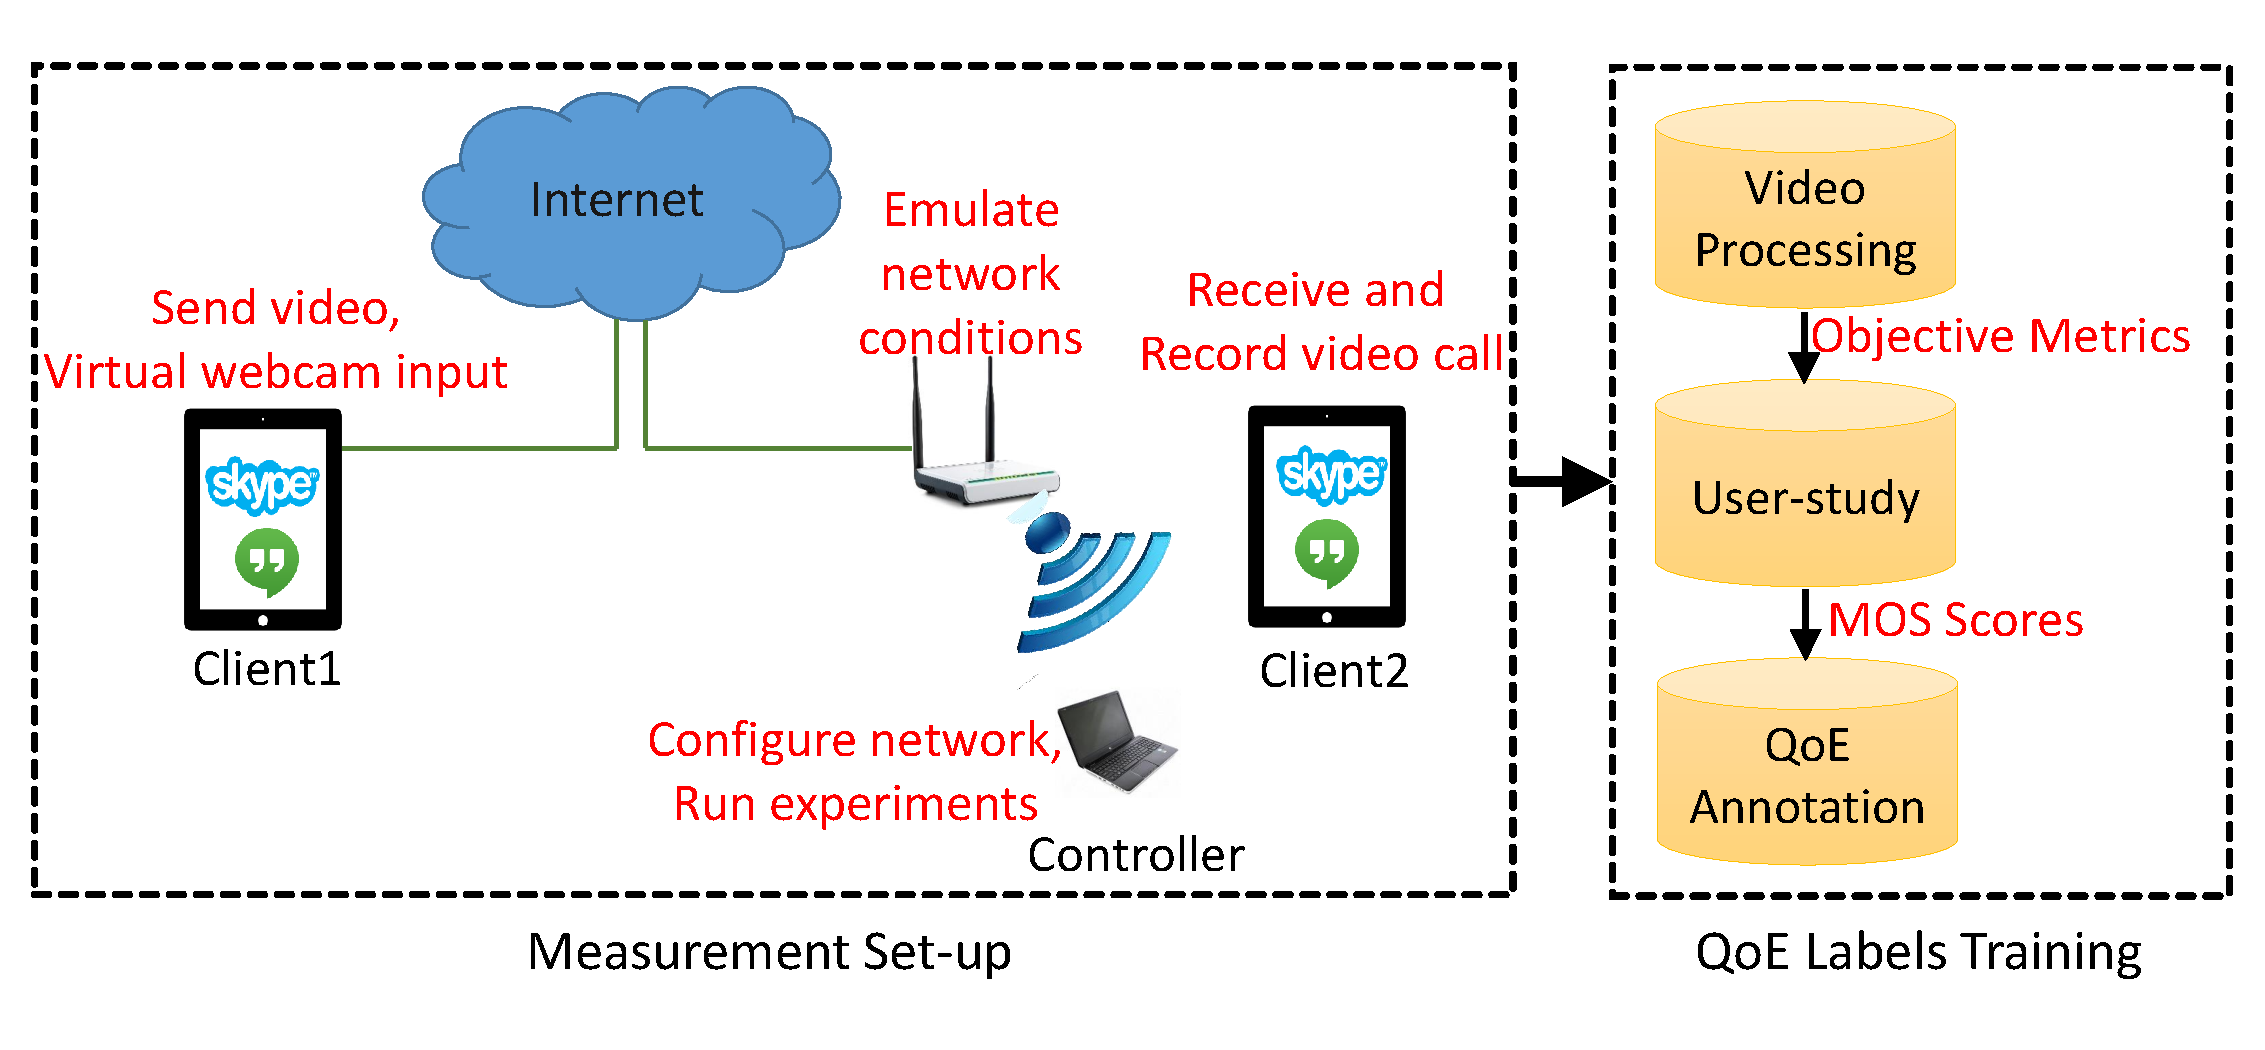
\includegraphics[width=\linewidth]{sections/network-work/setup}
     \vspace{-0.3in}
    \caption{Measurement set-up and system architecture. \textit{Left:} Video telephony measurements and recording video calls. \textit{Right:} Our framework processing recorded videos offline and extracting objective metrics to predict QoE labels.}
   \vspace{-0.2in}
  \label{fig:set-up}
\end{figure}
\begin{figure}[t]
  \centering
  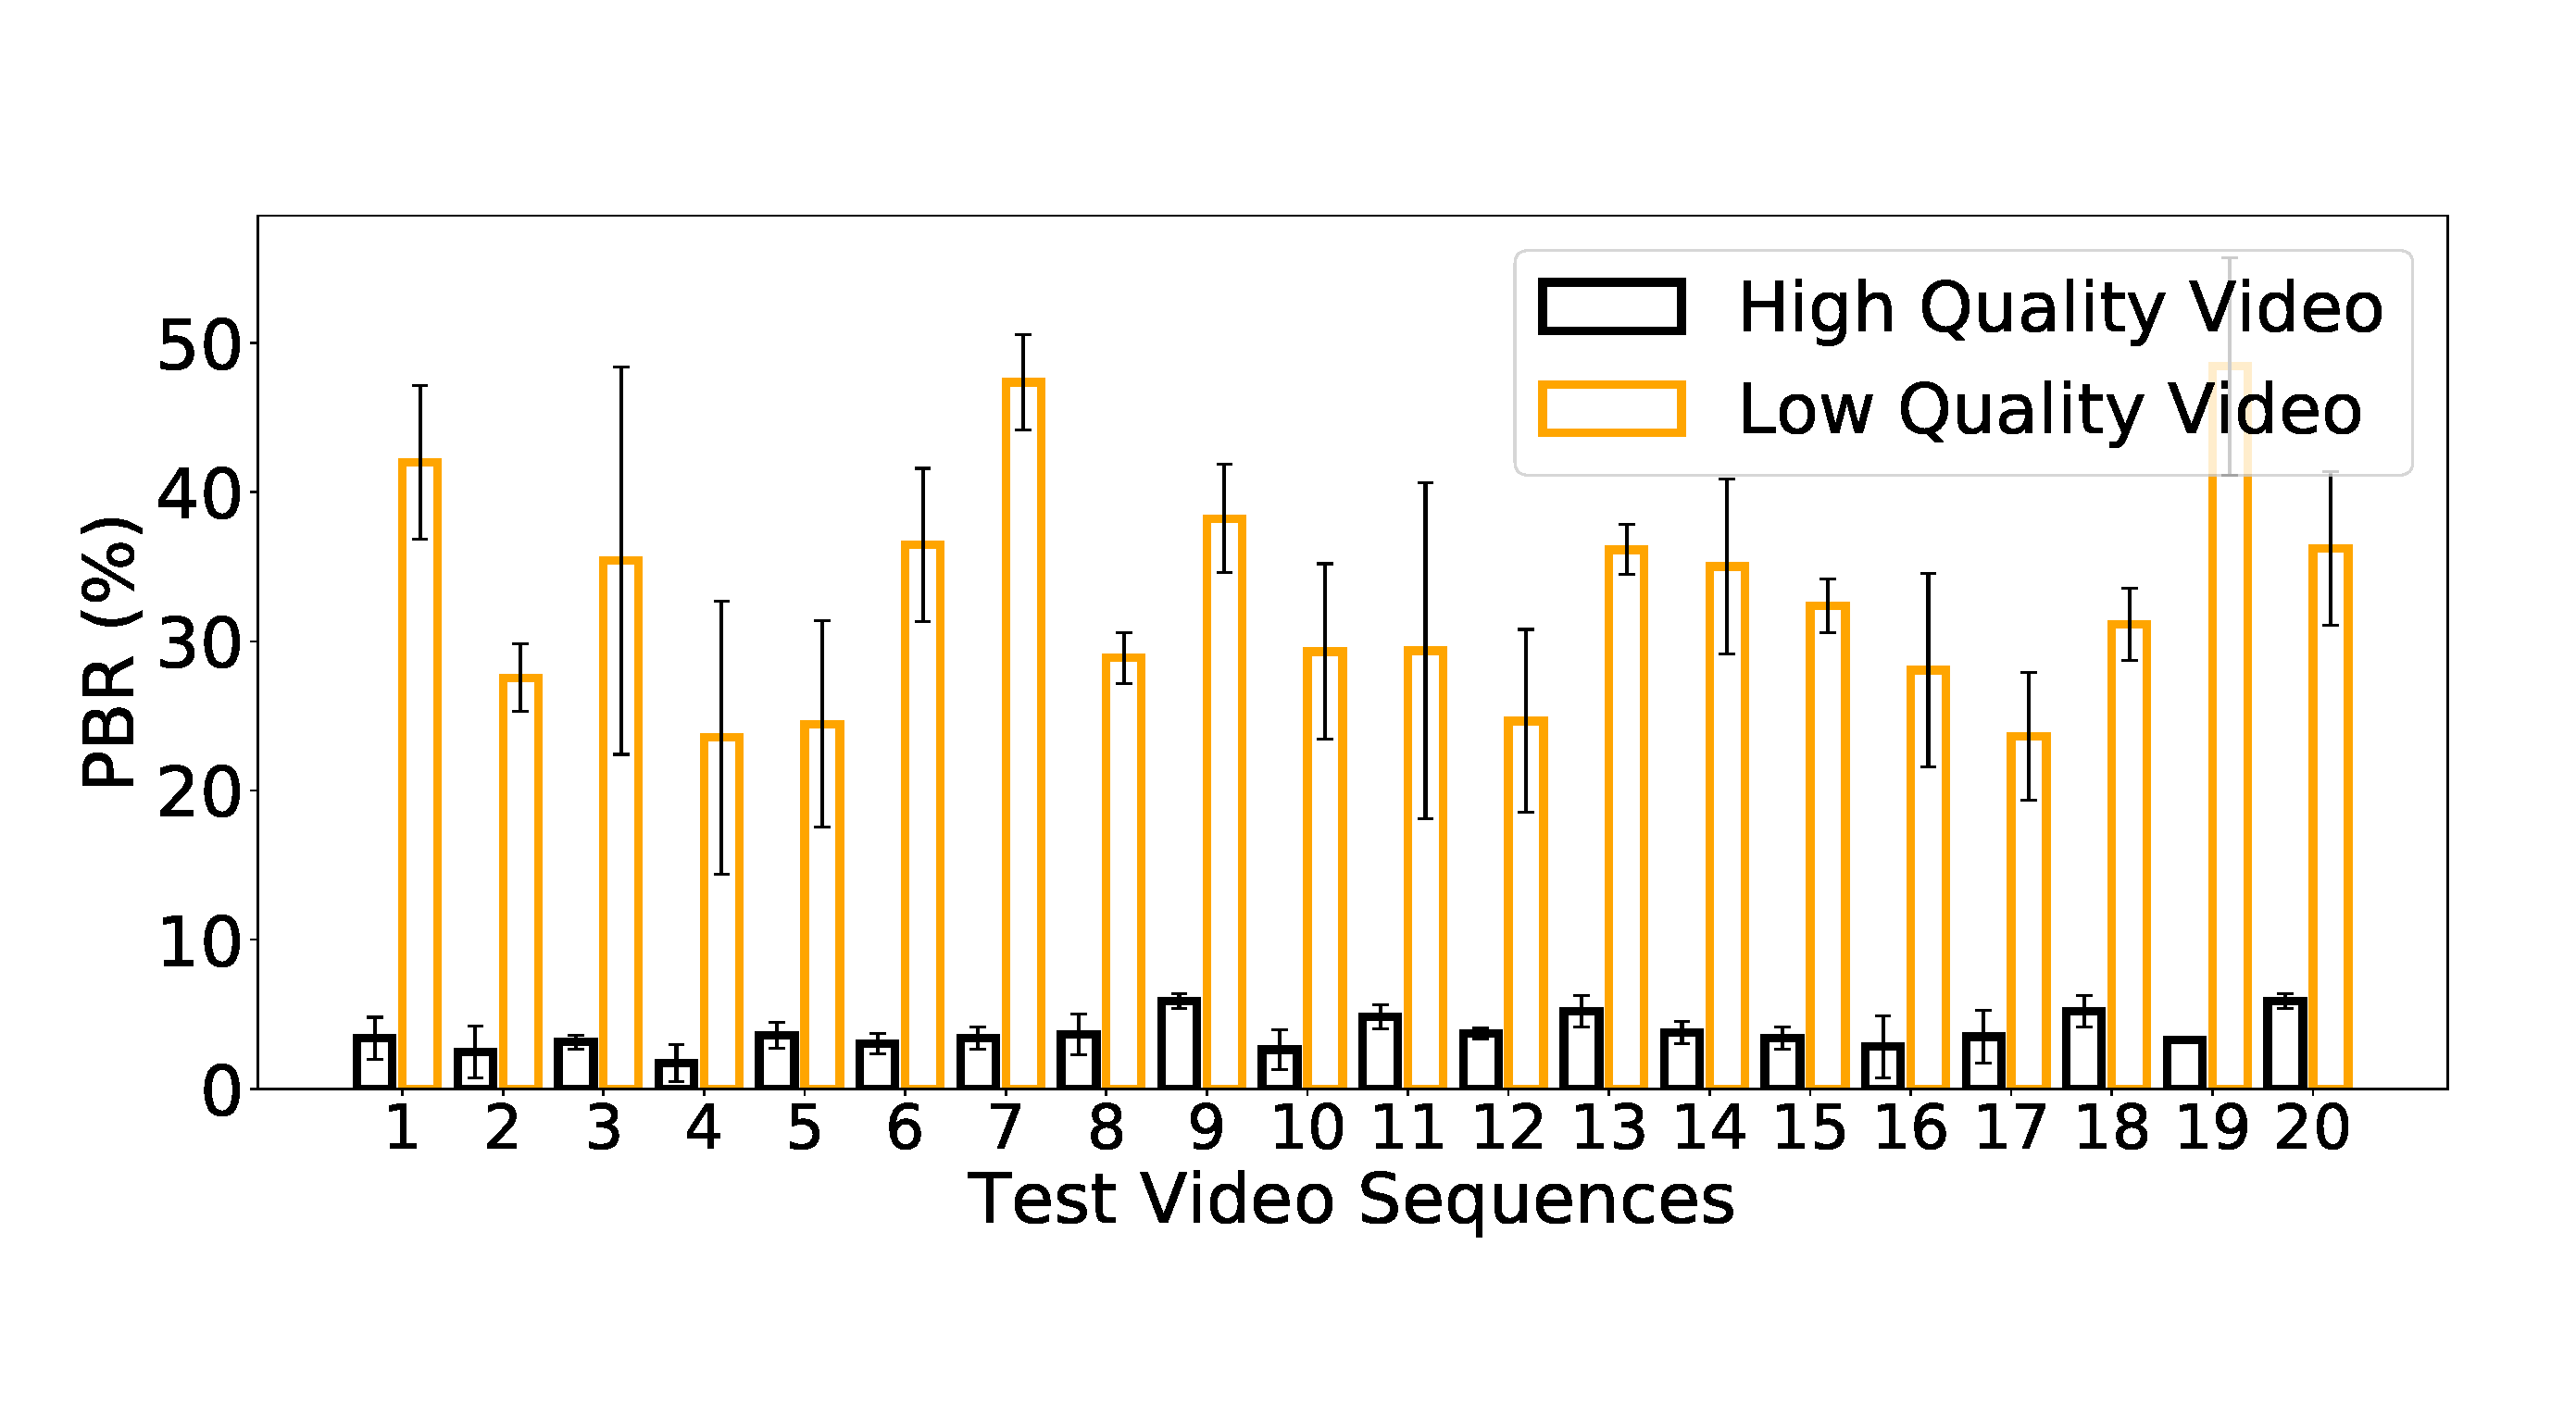
\includegraphics[width=\linewidth]{sections/network-work/bar-pbr}
   \vspace{-0.5in}
  \caption{Blur detection using PBR.}
\vspace{-2em}
  \label{fig:ourblurdetection}
\end{figure}

\section{Design for Scalable QoE Annotation} \label{label:design}
In this section, we first describe our framework and measurement methodology. 
We then explain our QoE metrics and evaluate them across different applications and devices. We validate that our metrics capture video artefacts caused by diverse network conditions.
\subsection{Measurement Methodology}

\noindent \textbf{Set-up:} 
In Figure~\ref{fig:set-up}, we show our measurement set-up and QoE labeling framework. 
Since video telephony is an interactive application, it requires at least two participating network end-points (clients). In our set-up, we use a mobile device on our local enterprise WiFi network (Client 1) and an Amazon-provided instance as the second end-point (Client 2). Both clients can run Skype or Hangouts\footnote{For FaceTime, we use 2 local clients (iPhone/iPad and MacBook Air) on different sub-networks, as creating virtual iOS and web-cam is challenging.}. 
When the video call is placed from Client 1 to Client 2, Client 2 runs a virtual web-cam that inputs a video file in telephony application instead of camera feed; at Client 1, the video is received during the call.
At the Amazon Client 2, we use \textit{manycam} \cite{mancam}, a virtual web-cam tool. 
This tool can be used with multiple video applications in parallel for automation. 
In our LAN, a controller sits  to emulate diverse network conditions and to run experiments on the connected mobile device  through Android debug bridge (ADB) interface (via USB or WiFi connection). 
To automate the video call process, we use AndroidViewClient (AVC) library \cite{awc}.
Once the received call is accepted, we start the screen recording of the video call session.   The videos are recorded using Az screen recorder \cite{azscreen}. 
The recorded videos are sent to video processing module to calculate the objective QoE metrics. 
We use Ffmpeg \cite{ffmpeg} tool to extract our QoE metrics. Ffmpeg is a video framework with large collection of coding libraries. To validate our metrics and translate them into user experience, the videos are then shown to users to rate their experience. 
Finally, we retrieve MOS from all users and map our QoE metrics to MOS. We delve into the details of our user  study and modeling in Section~\ref{label:results}.
%We use Ffmpeg to convert, encode and manipulate videos to extract Rbitrate, RFps and freeze ratio etc. 
%We use Matlab and OpenCV to convert video to images and extract blur metric of individual images.

%\begin{table}[t]
%  \centering
%    \scalebox{1.08}{
%  \begin{tabular}{c|c|c|c|c}
%  \hline \hline
%    \textbf{Video Sequence} & \textbf{Frames} & \textbf{Fps} & \textbf{bitrate (Kbps)} & \textbf{Motion} \\
%    \hline
%    \hline
%     $TalkShow.y4m$ & 600 & 40 & 1360 & low \\ \hline
%     $Bunny.y4m$ & 504 & 25 & 3500 & average \\ \hline
%     $Bus.y4m$ & 500 & 12 & 19037 & high \\ \hline
%  \end{tabular}
%    }
%  \caption{Motion classification based on Video Coding Parameters and Corresponding QoE Ground-truth}
%  \label{tab:table2}
%\end{table}

\begin{figure*}
%    \centering
%    \vspace*{-1em}
%    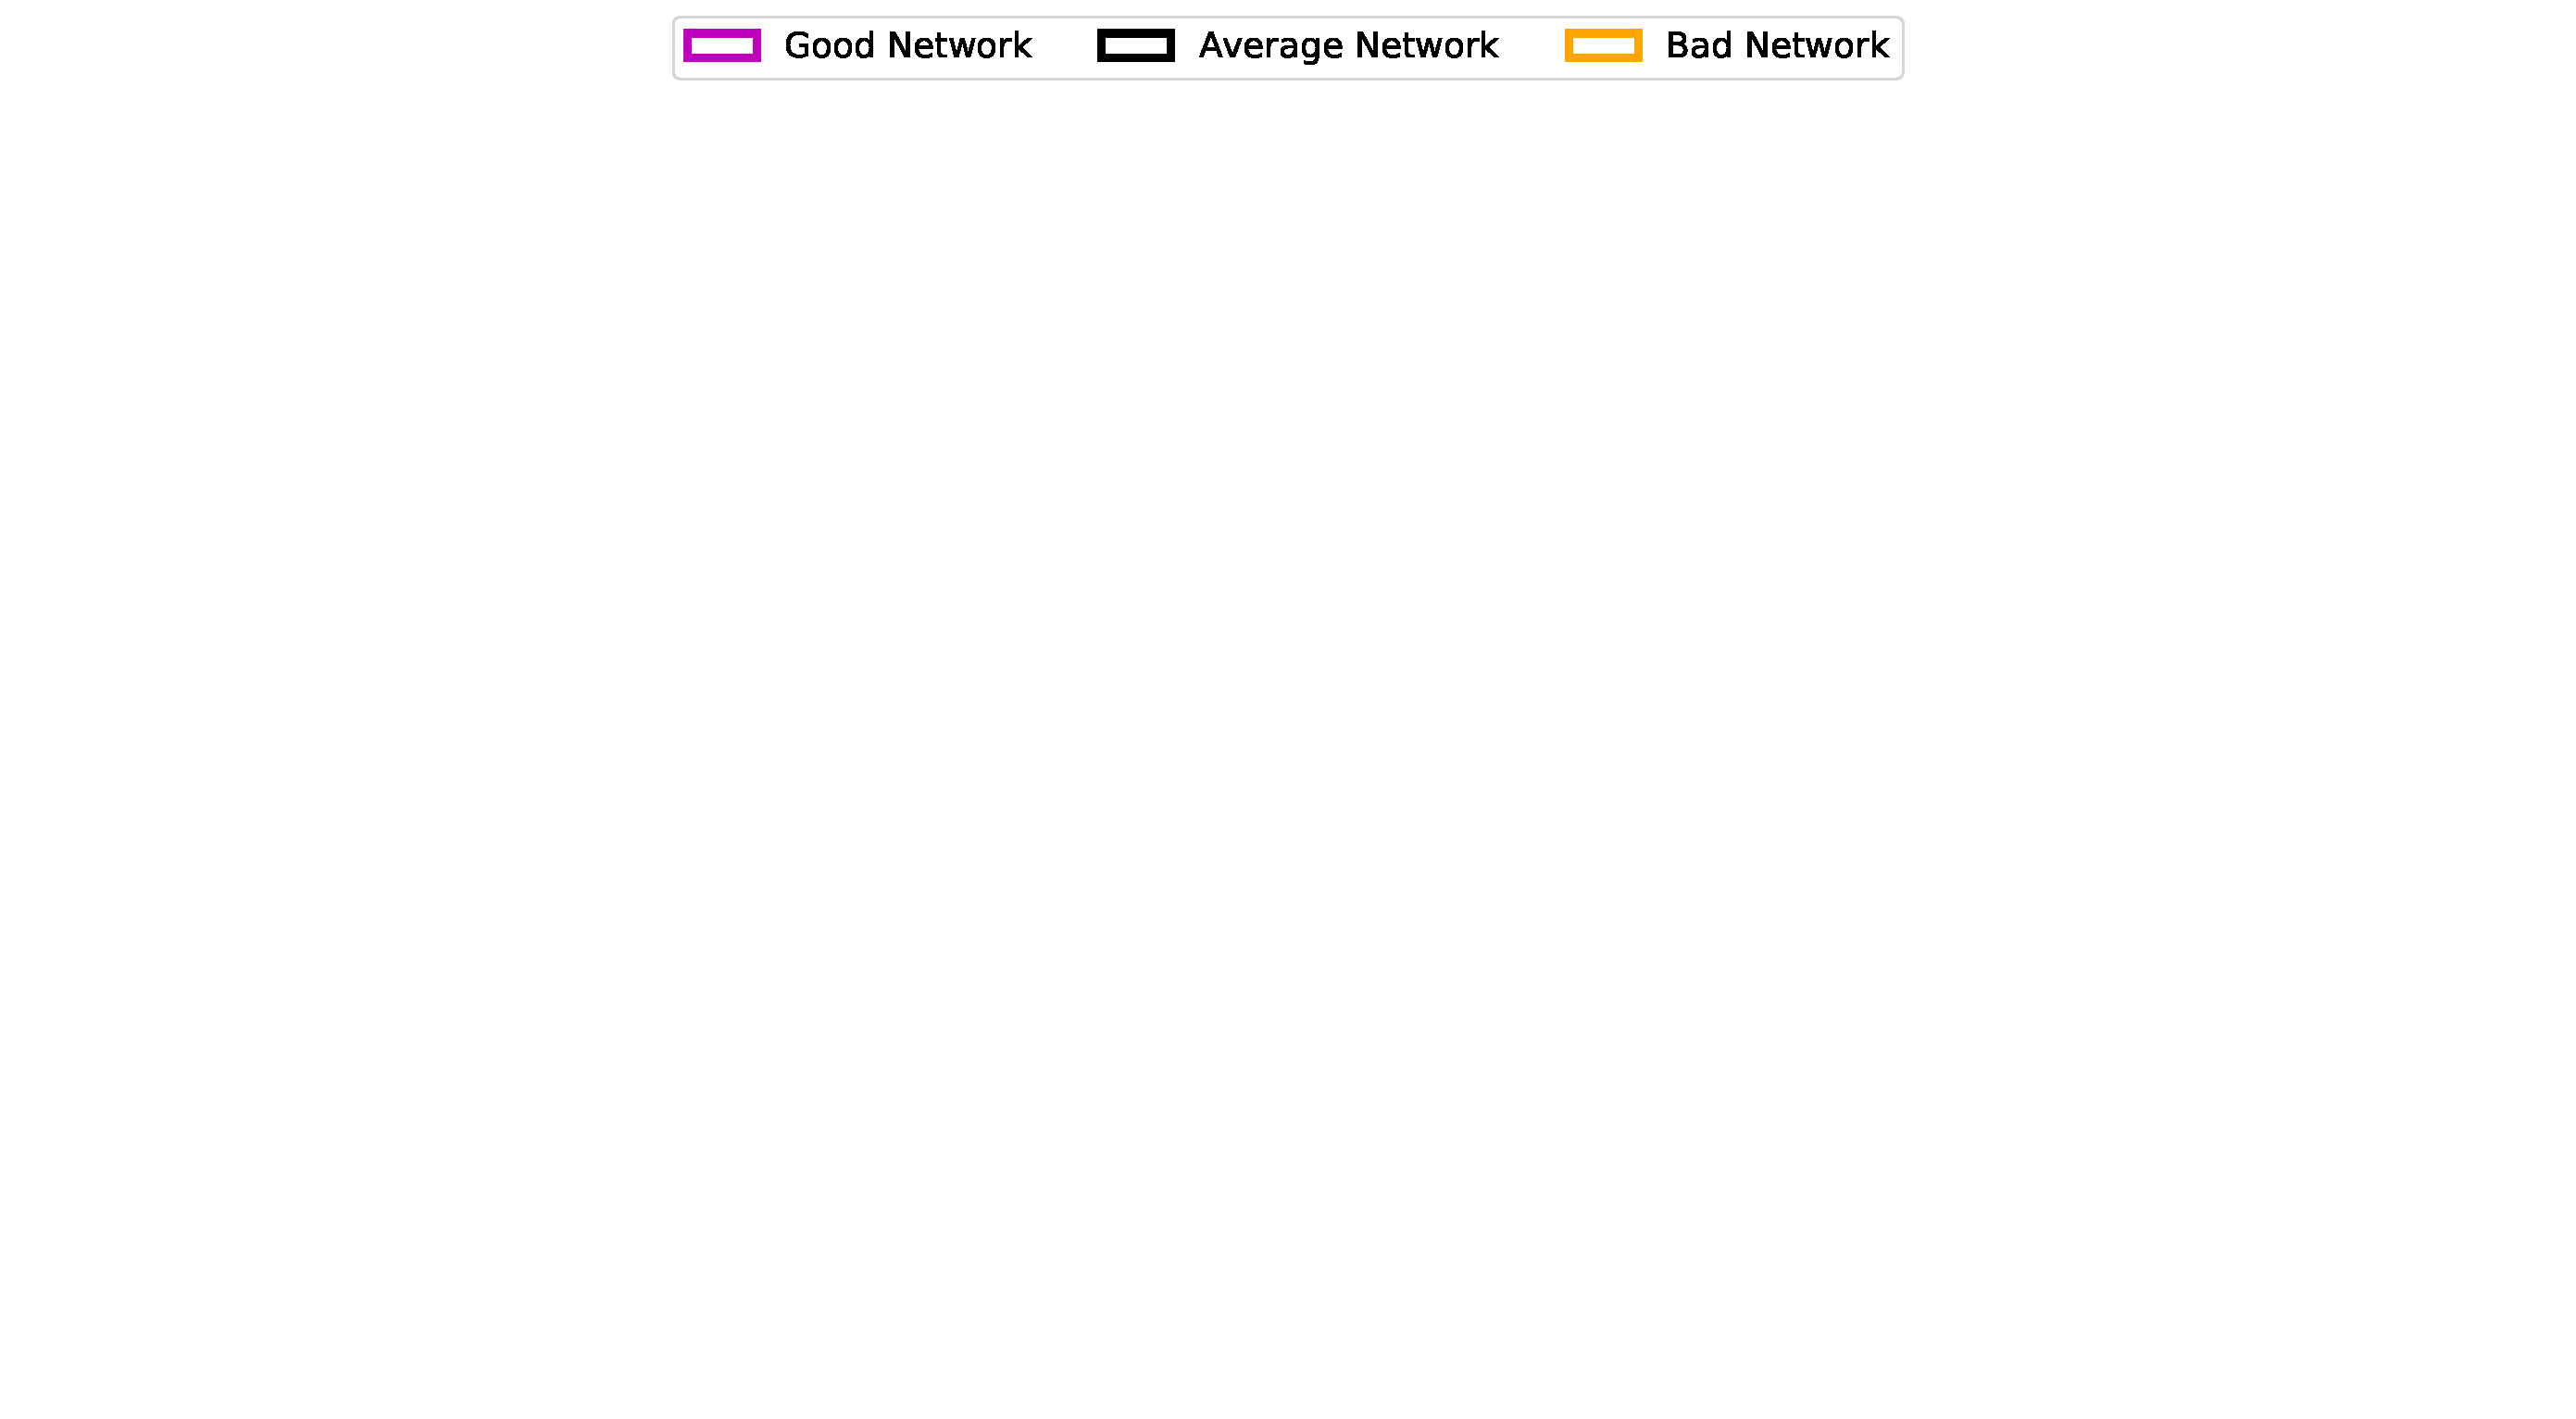
\includegraphics[trim={2.5cm 24.5cm 2.5cm 0},clip,width=0.8\linewidth]{sections/network-work/legend4.pdf}
%  \subfigure[Content and Motion]{\hspace*{-1em}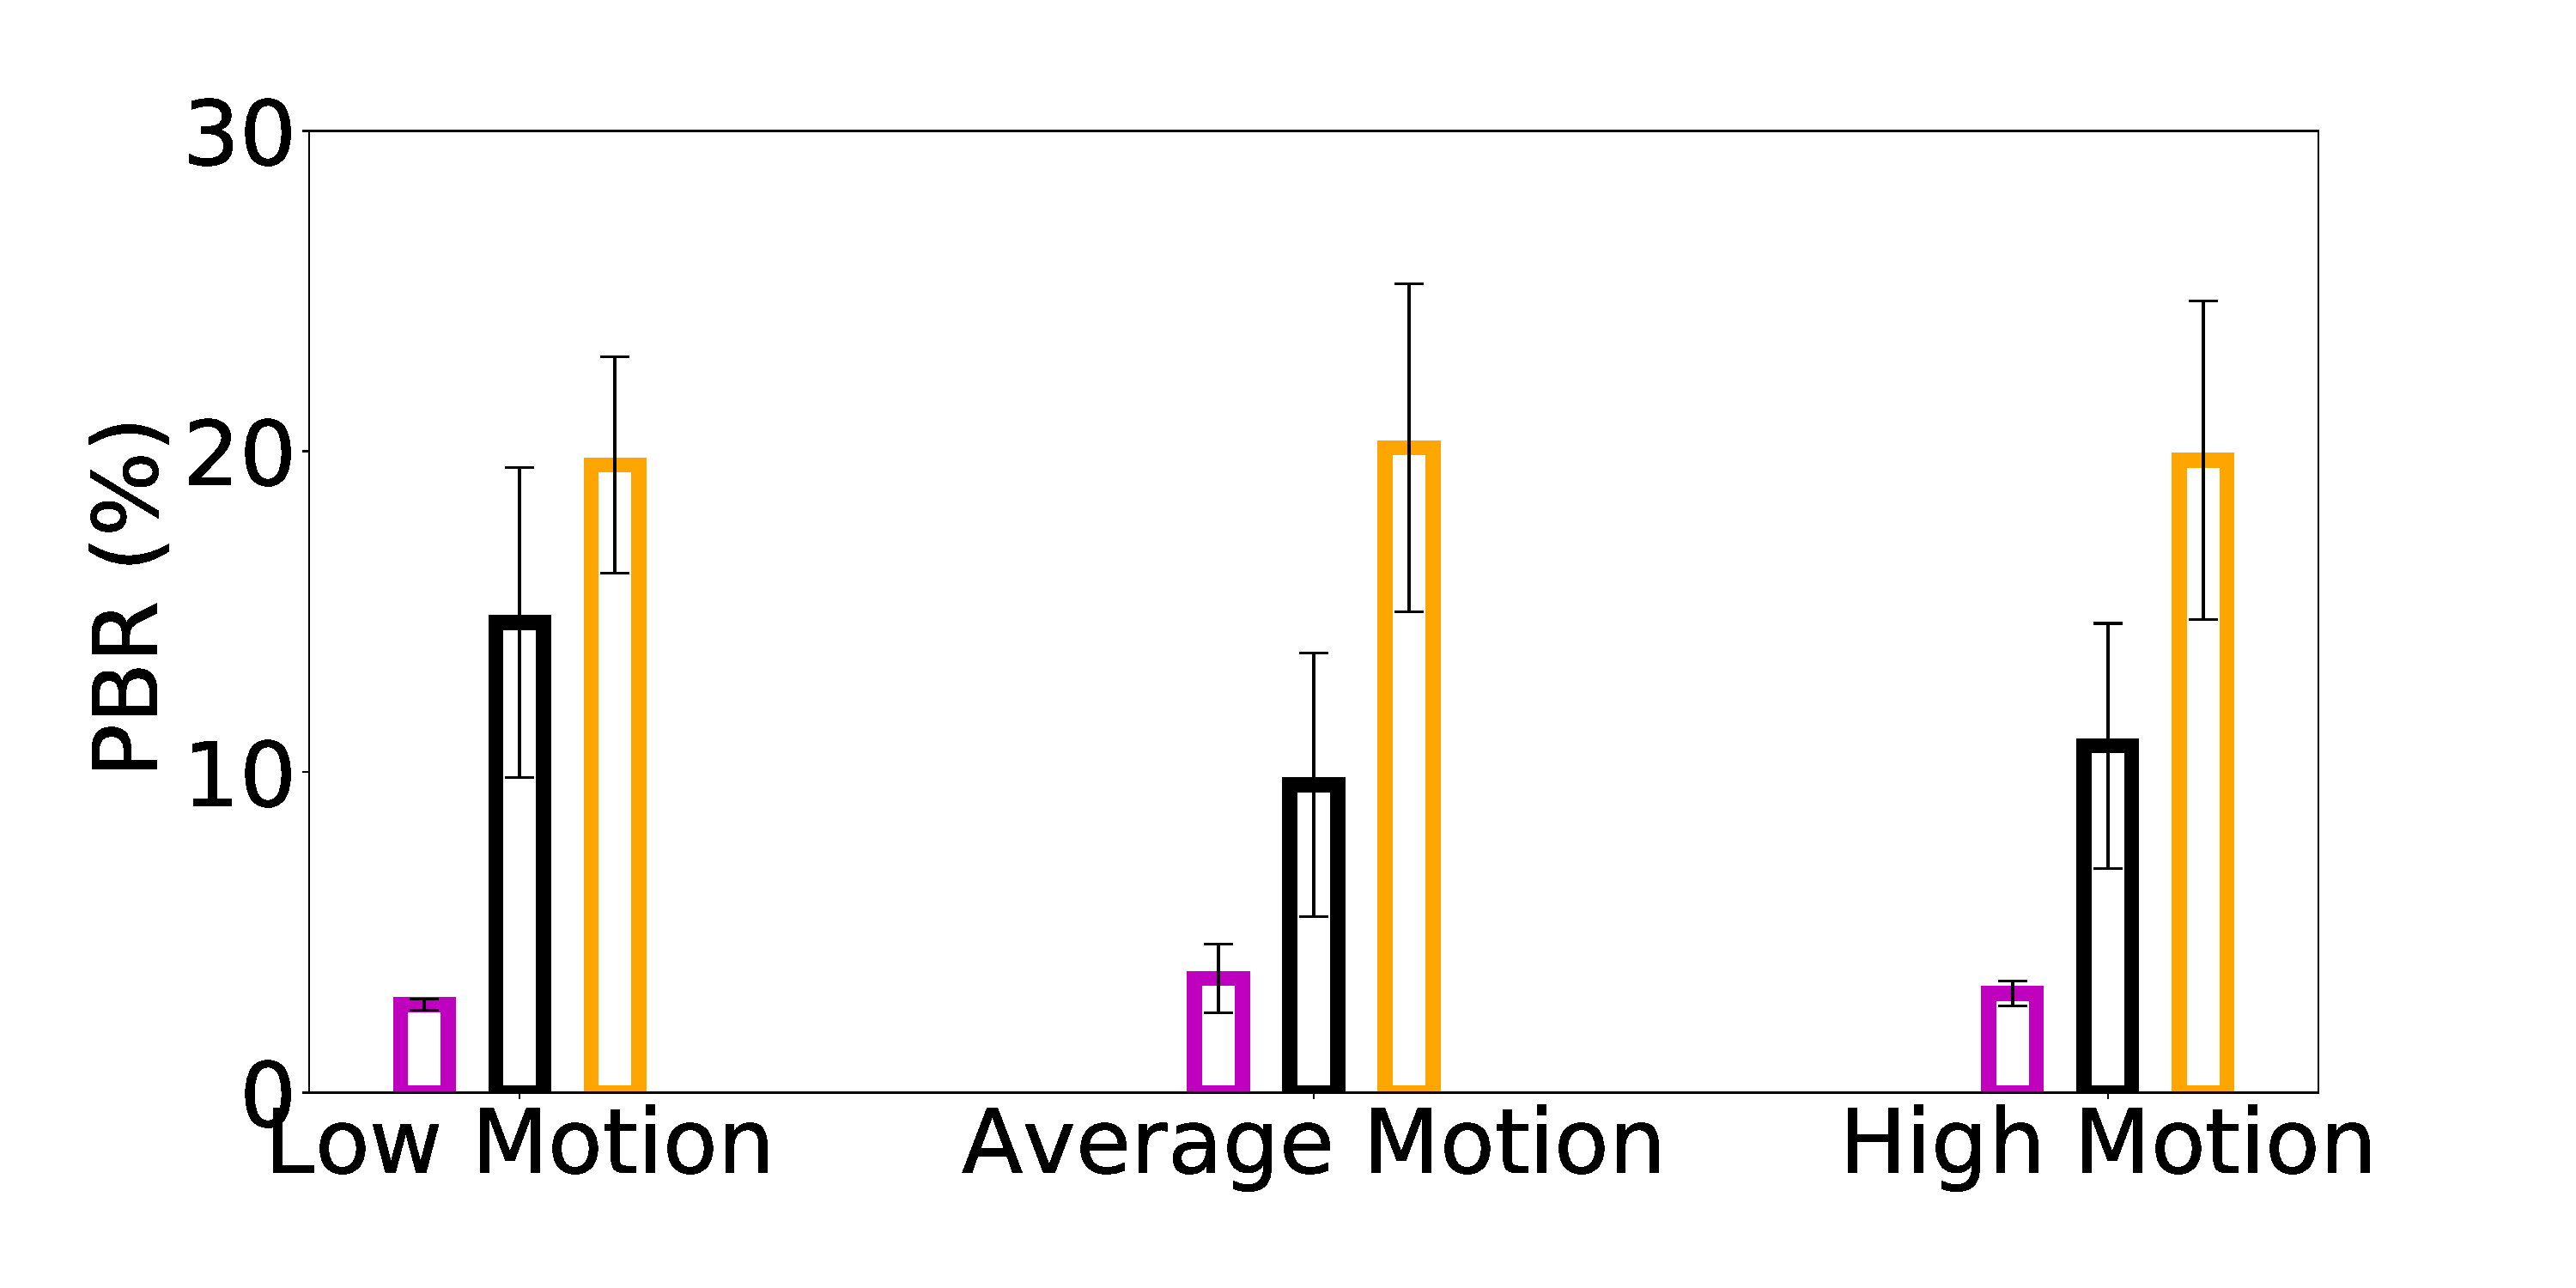
\includegraphics[width=0.33\textwidth]{sections/network-work/content-bitrate}\label{fig:cont-pbr} \vspace*{-3em}}~
%  \subfigure[Applications]{\hspace*{-1em}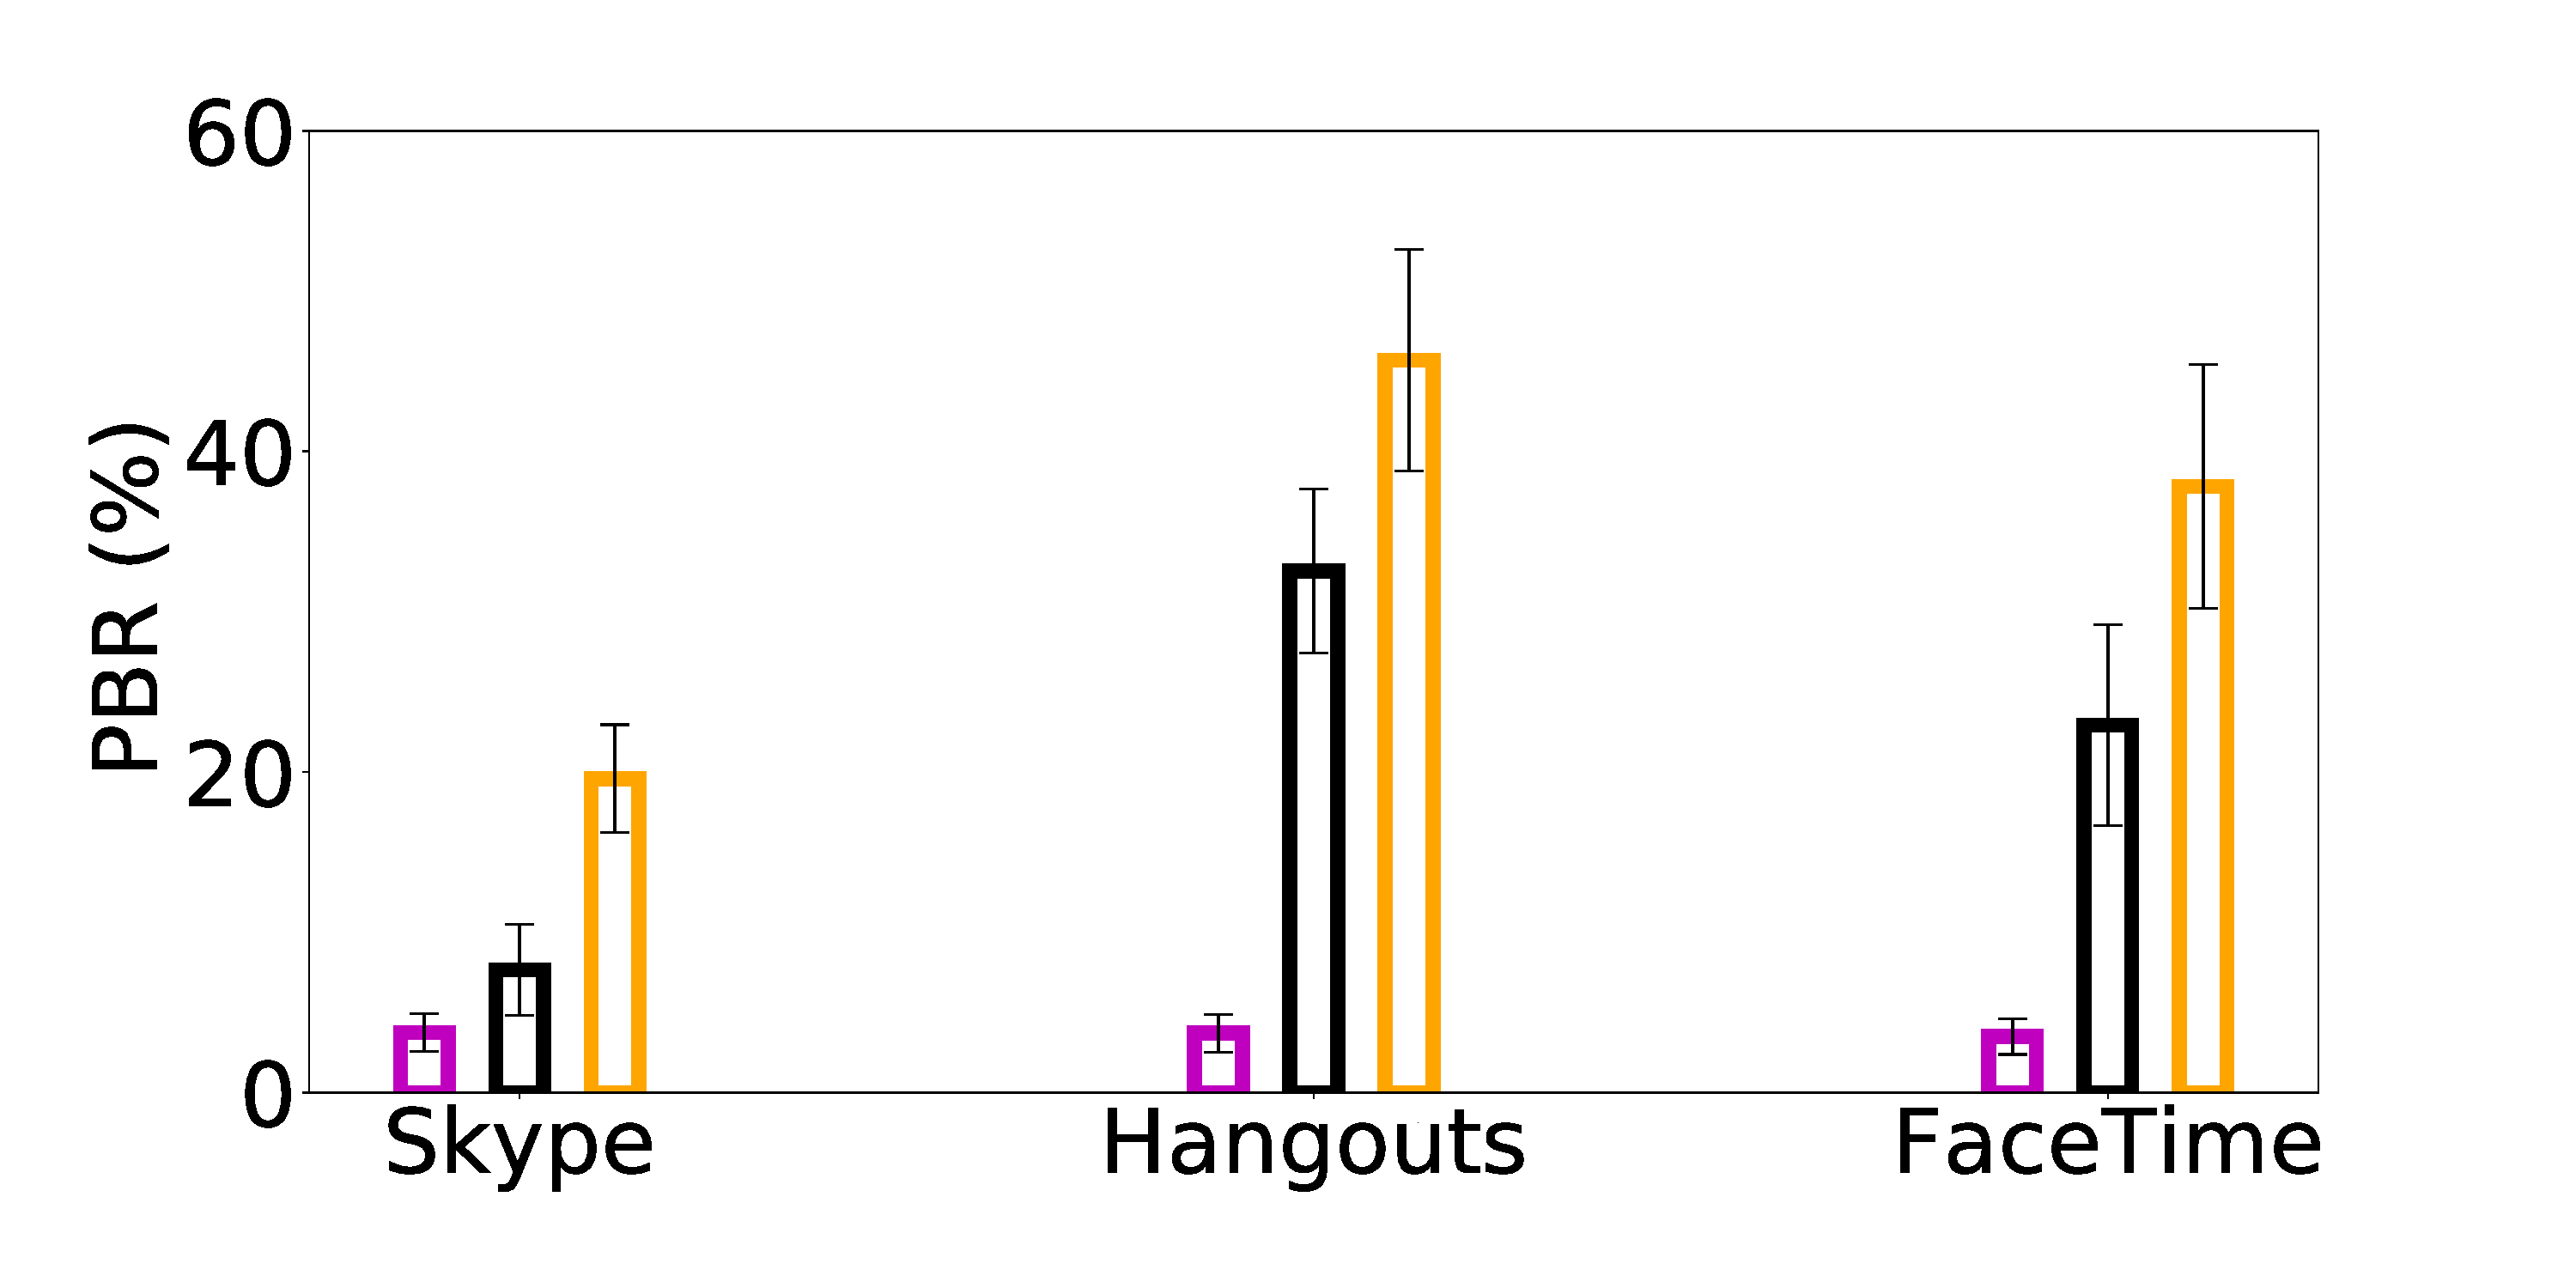
\includegraphics[width=0.33\textwidth]{sections/network-work/app-bitrate}\label{fig:app-pbr} \vspace*{-3em}}~
%   \subfigure[Devices] {\hspace*{-1em} 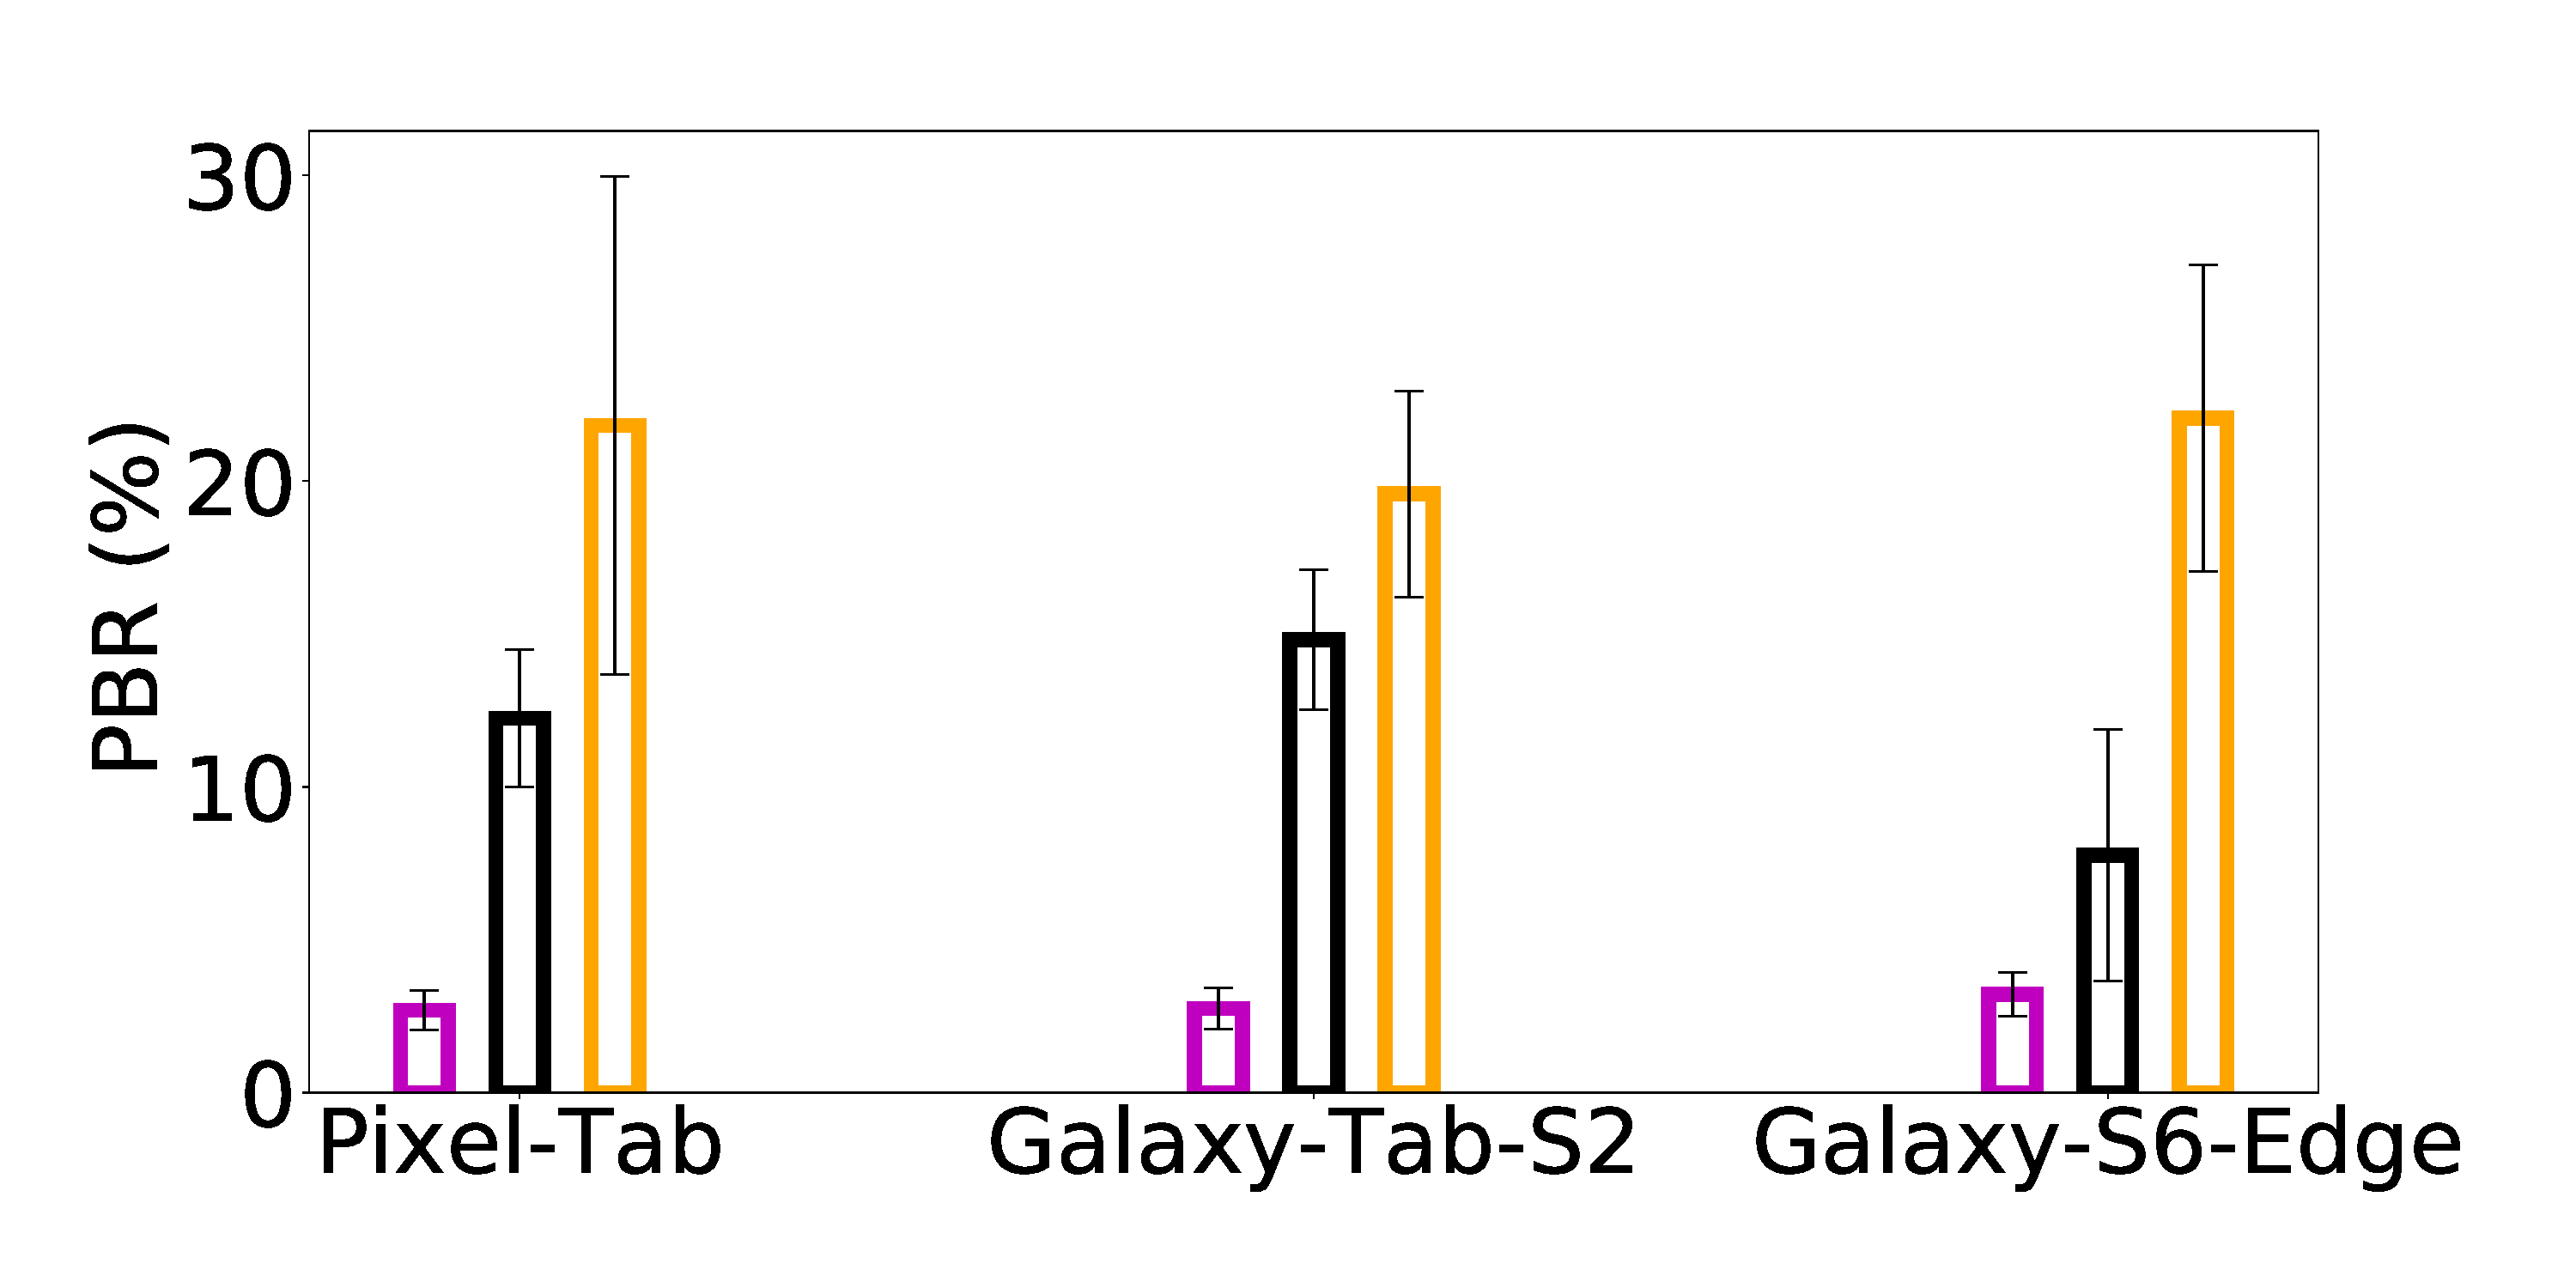
\includegraphics[width=0.33\textwidth]{sections/network-work/dev-bitrate}\label{fig:dev-pbr} \vspace*{-3em}}
%     \subfigure[Content and Motion]{\hspace*{-1em}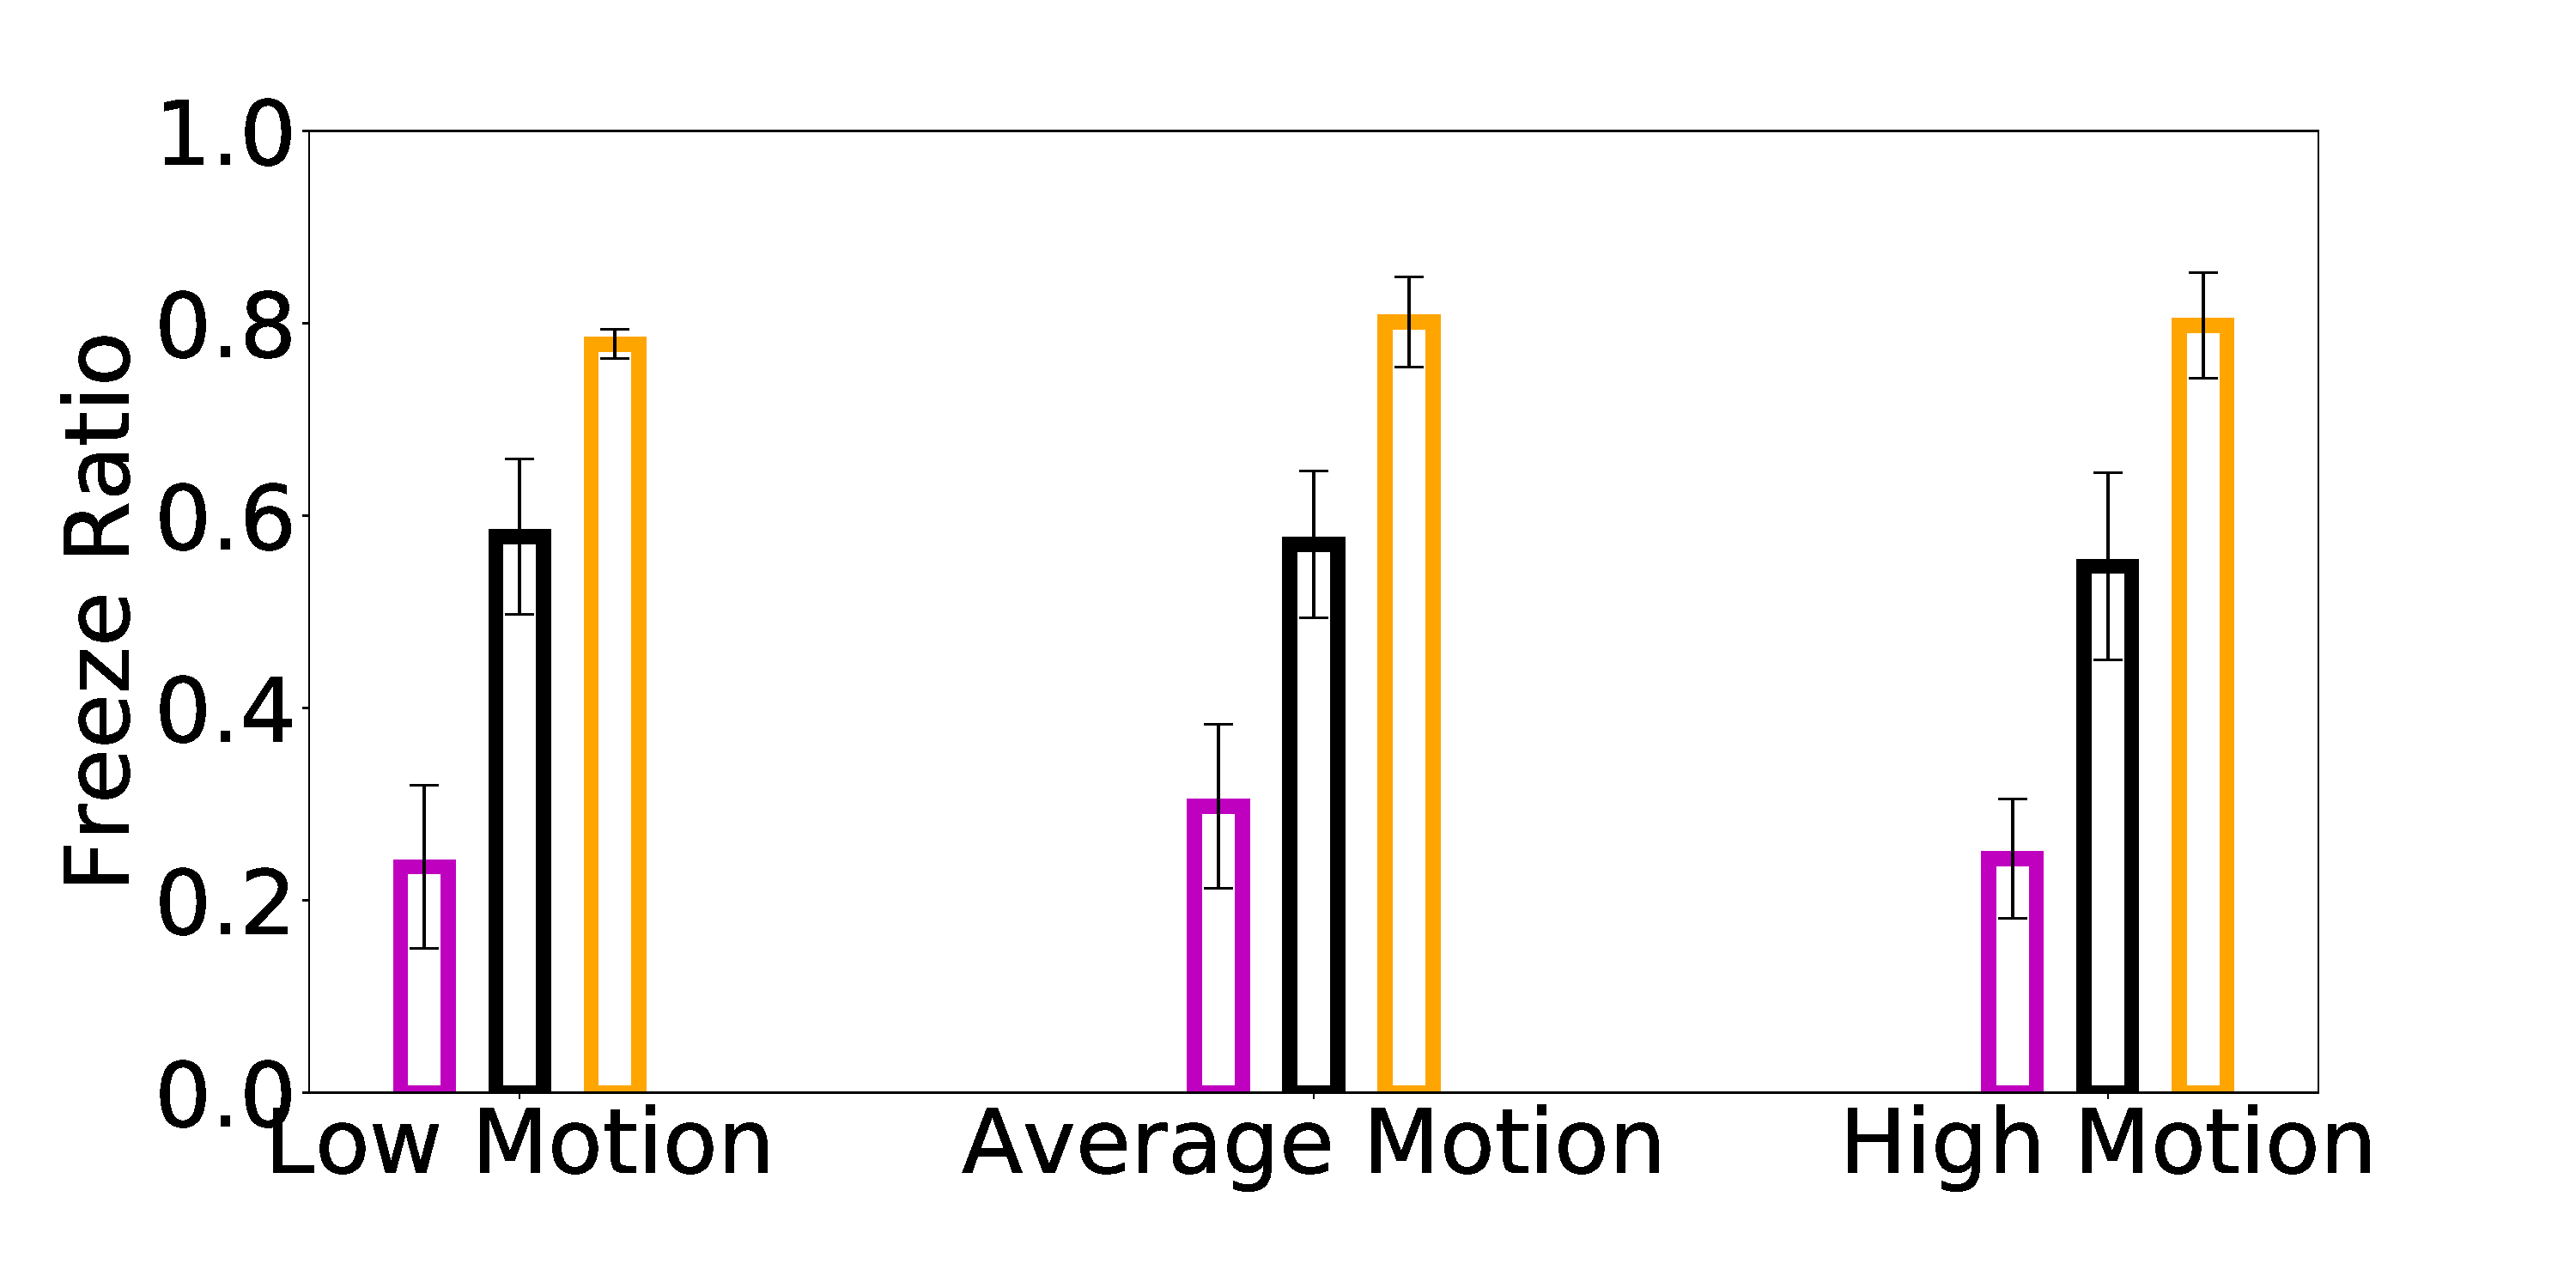
\includegraphics[width=0.33\textwidth]{sections/network-work/content-stutter}\label{fig:cont-st}}~
%     \subfigure[Applications]{\hspace*{-1em}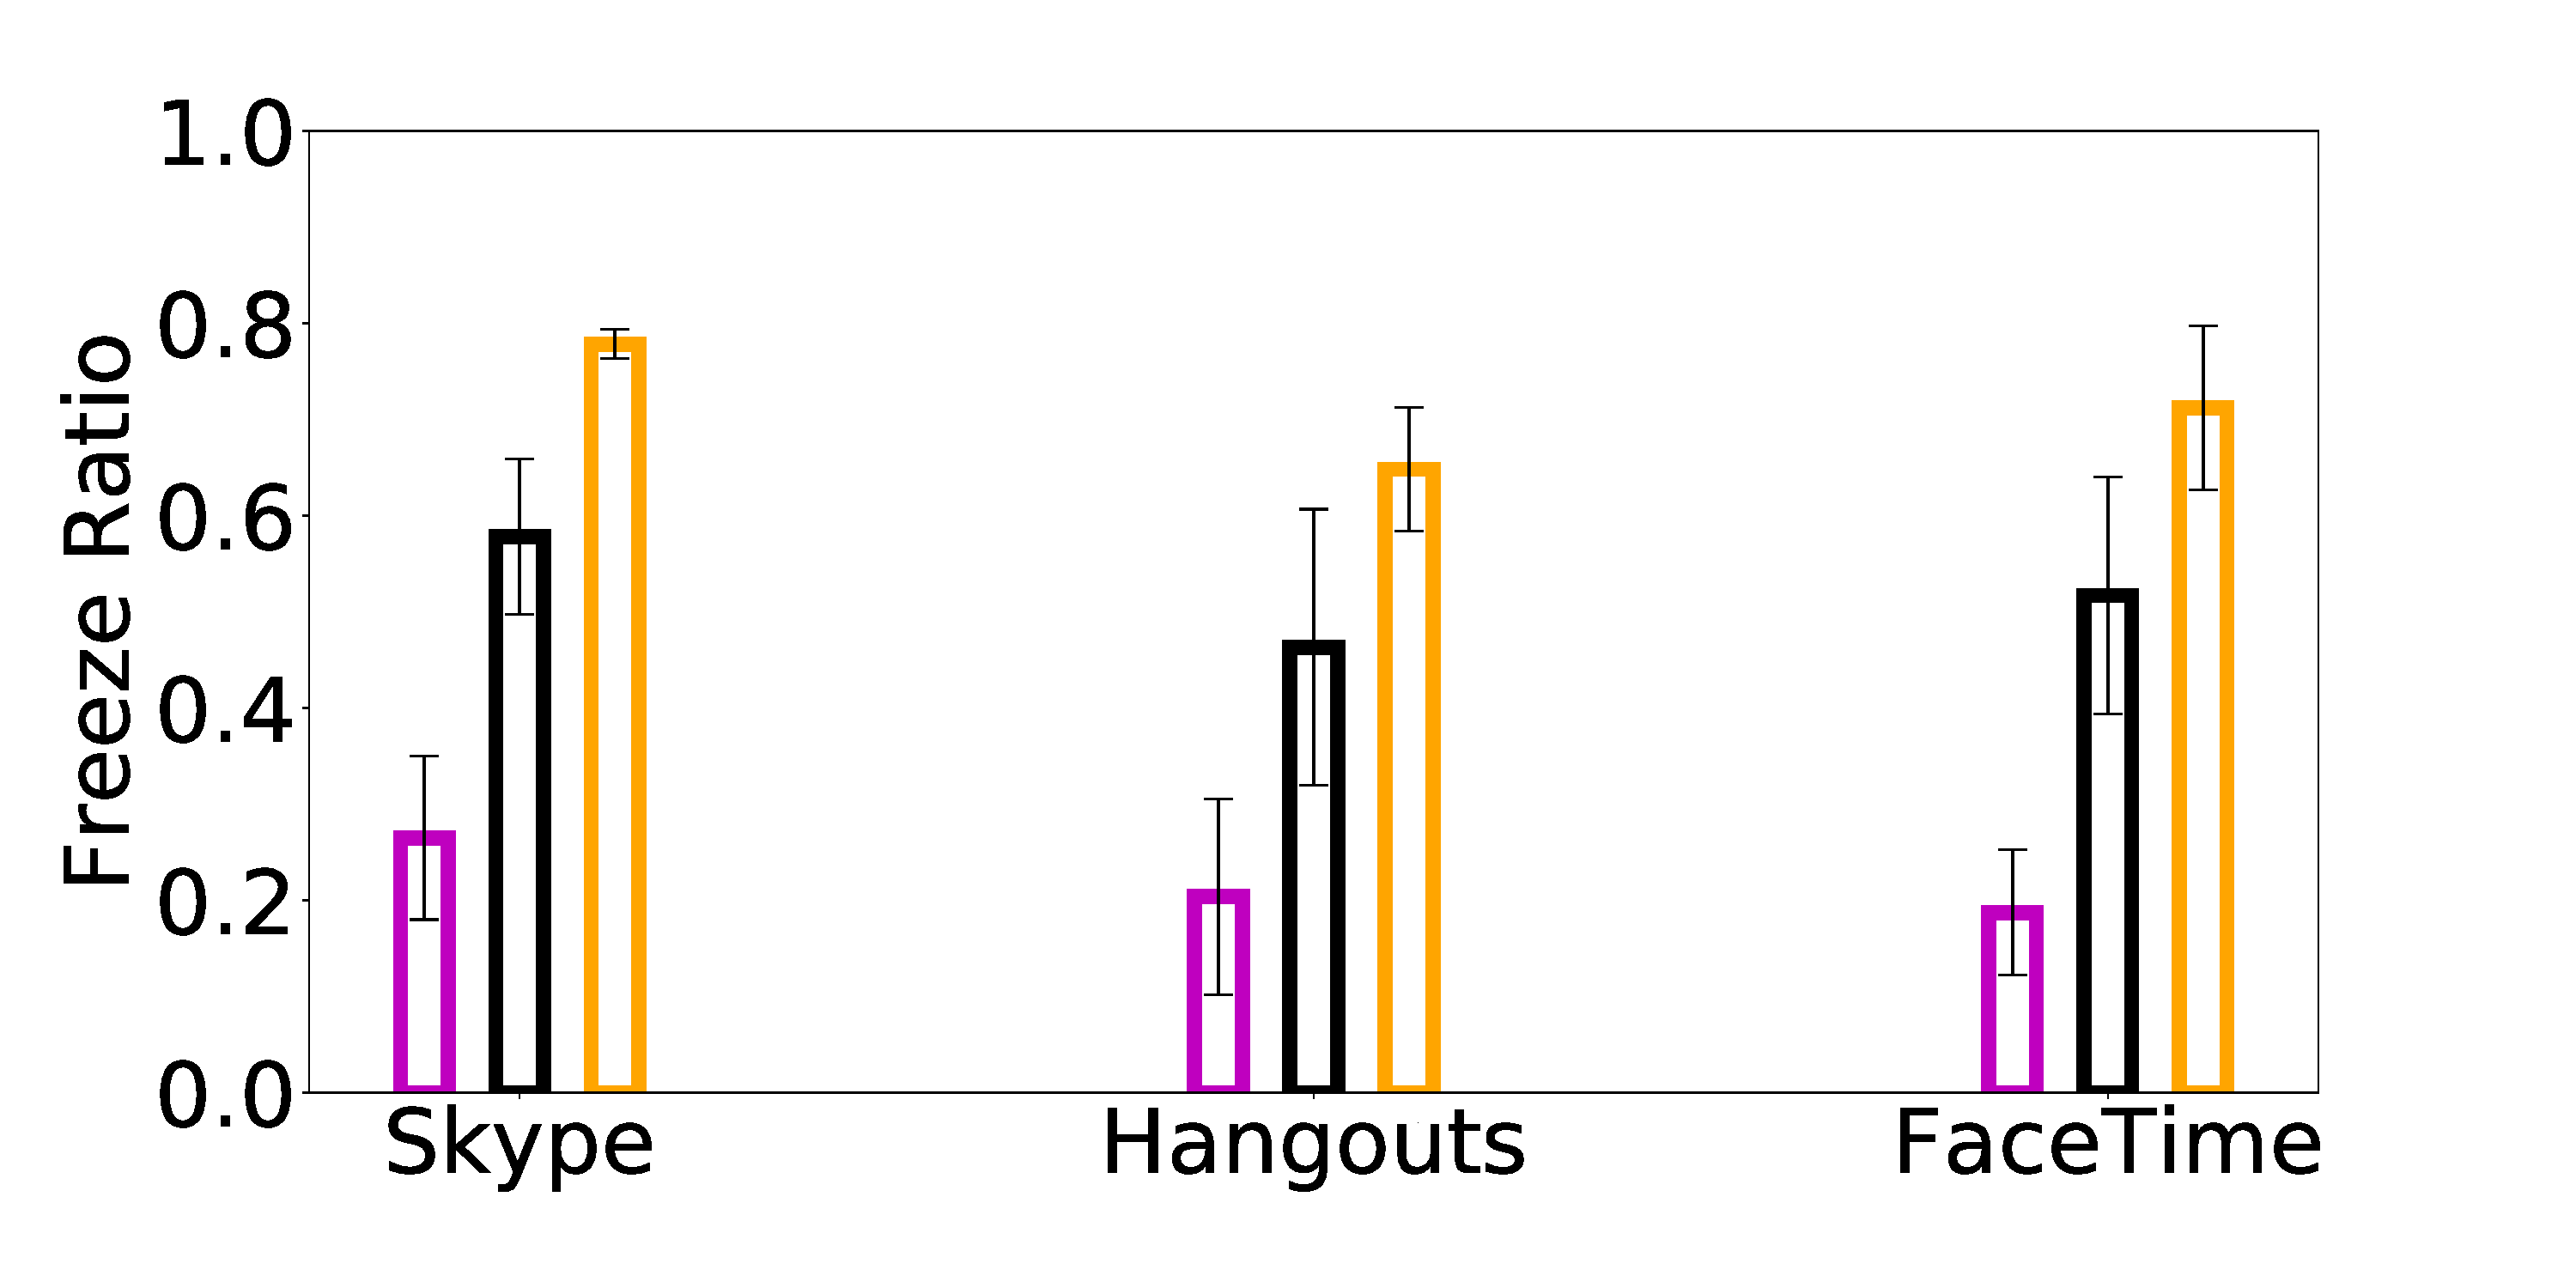
\includegraphics[width=0.33\textwidth]{sections/network-work/app-stutter}\label{fig:app-st}}~
%     \subfigure[Devices] {\hspace*{-1em} 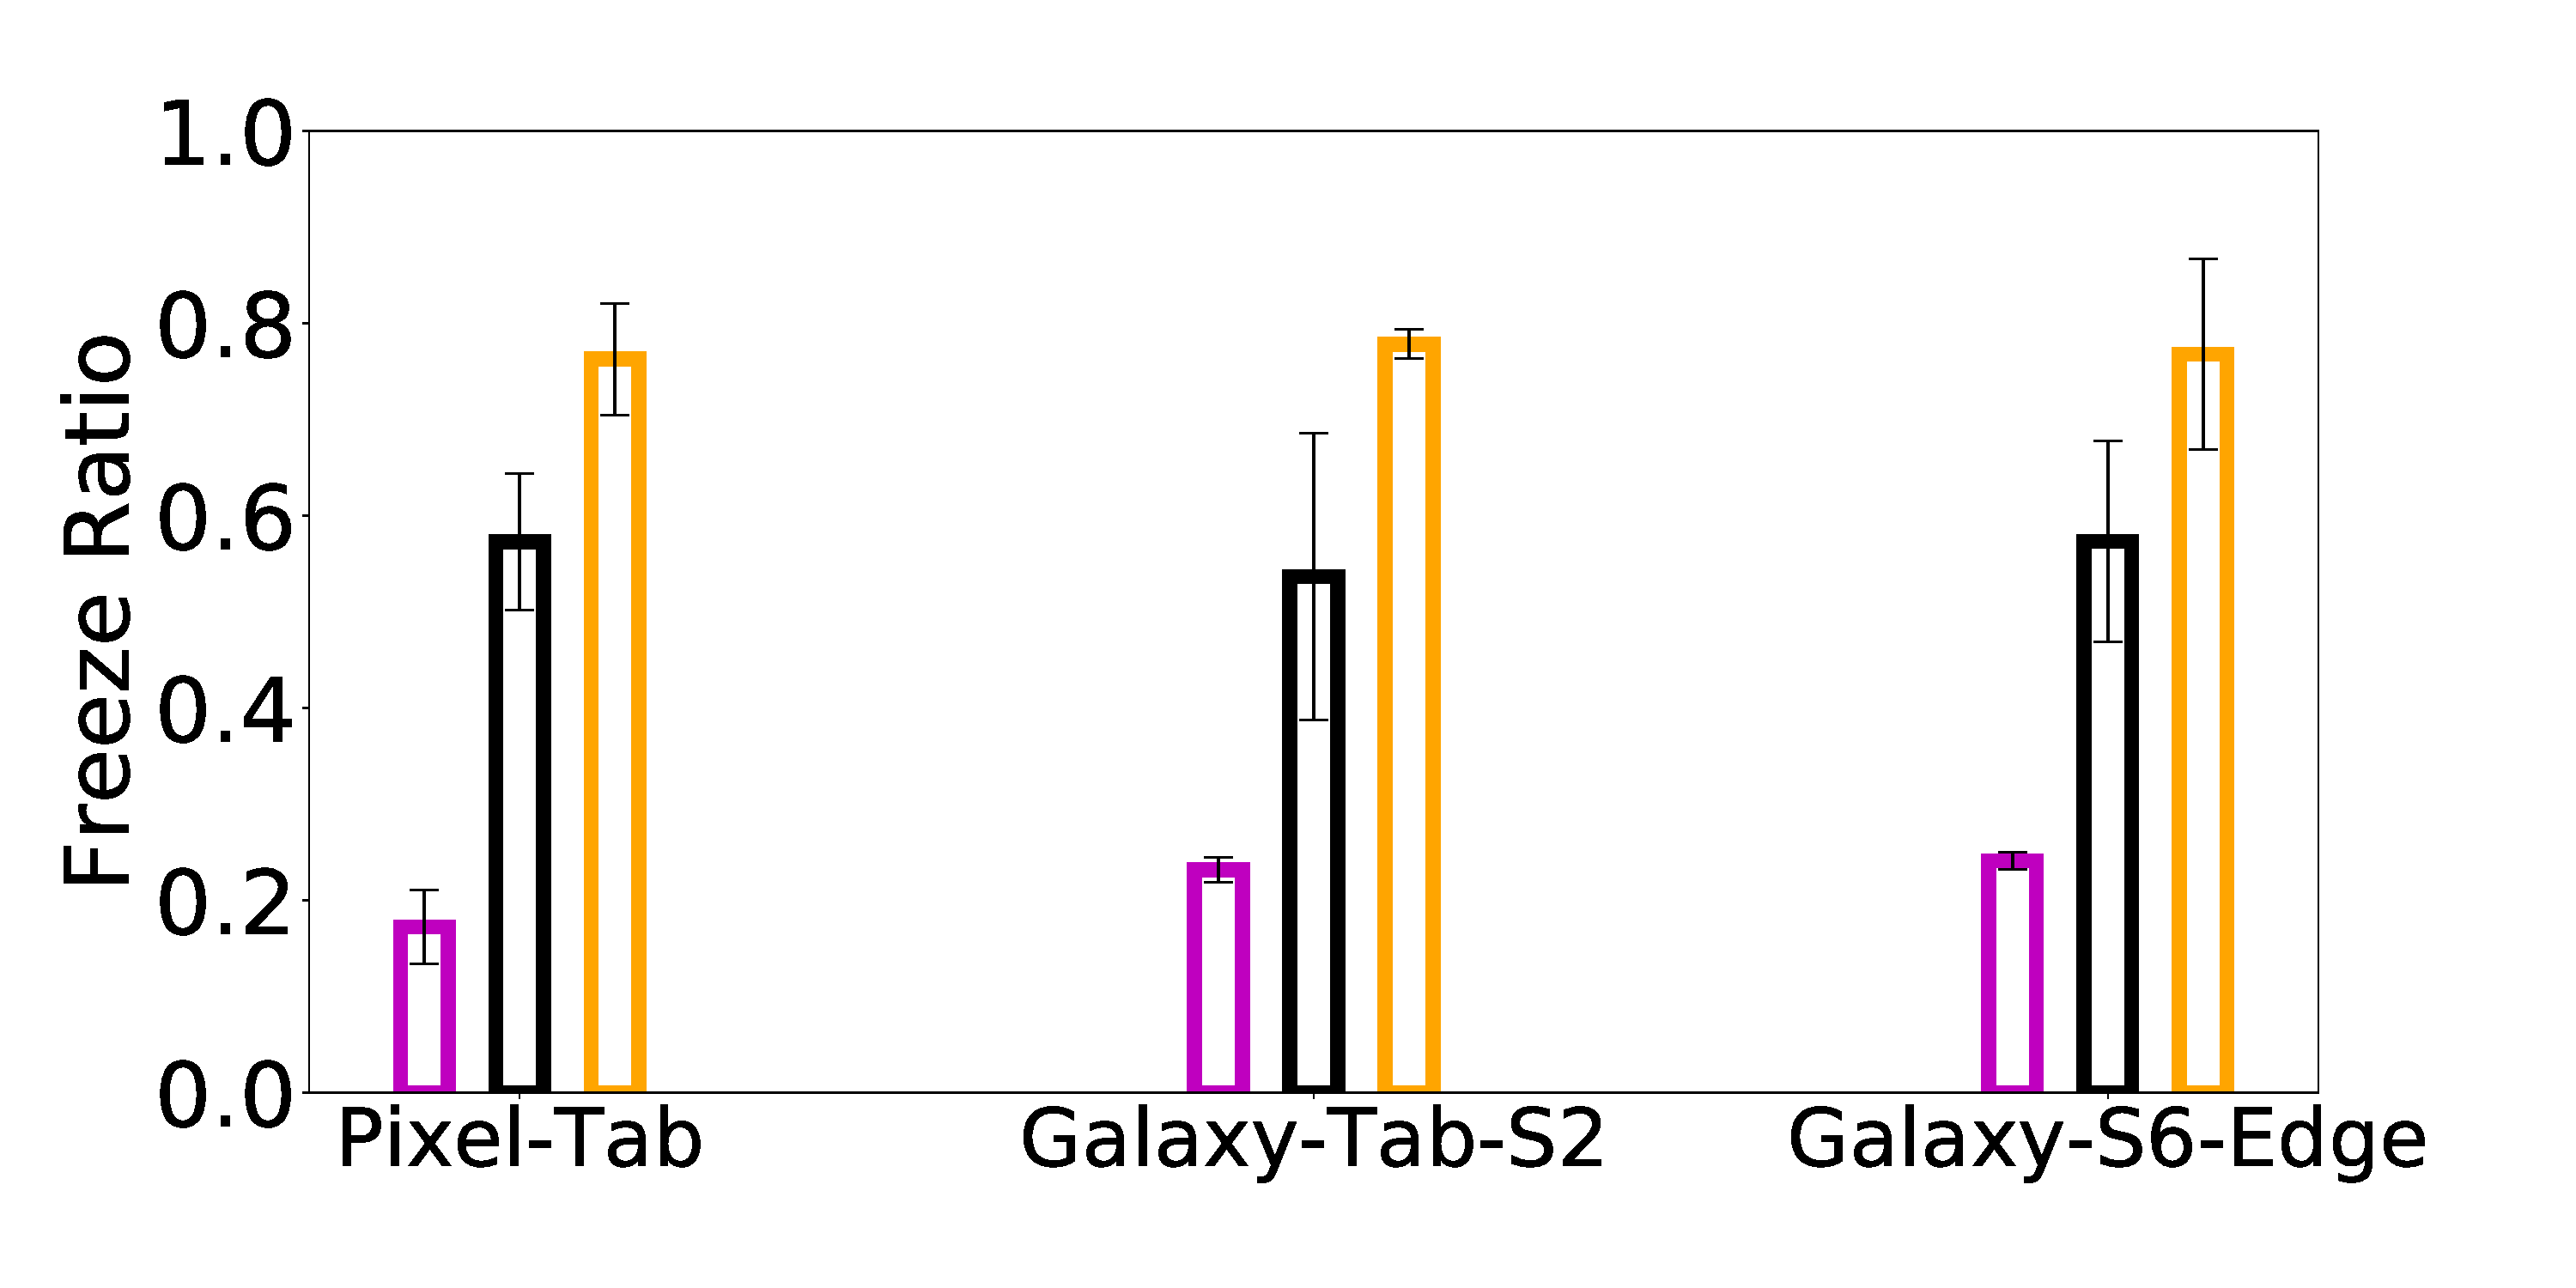
\includegraphics[width=0.33\textwidth]{sections/network-work/dev-stutter} \label{fig:dev-st}}
    \begin{subfigure}[b]{0.33\textwidth}
        \centering
        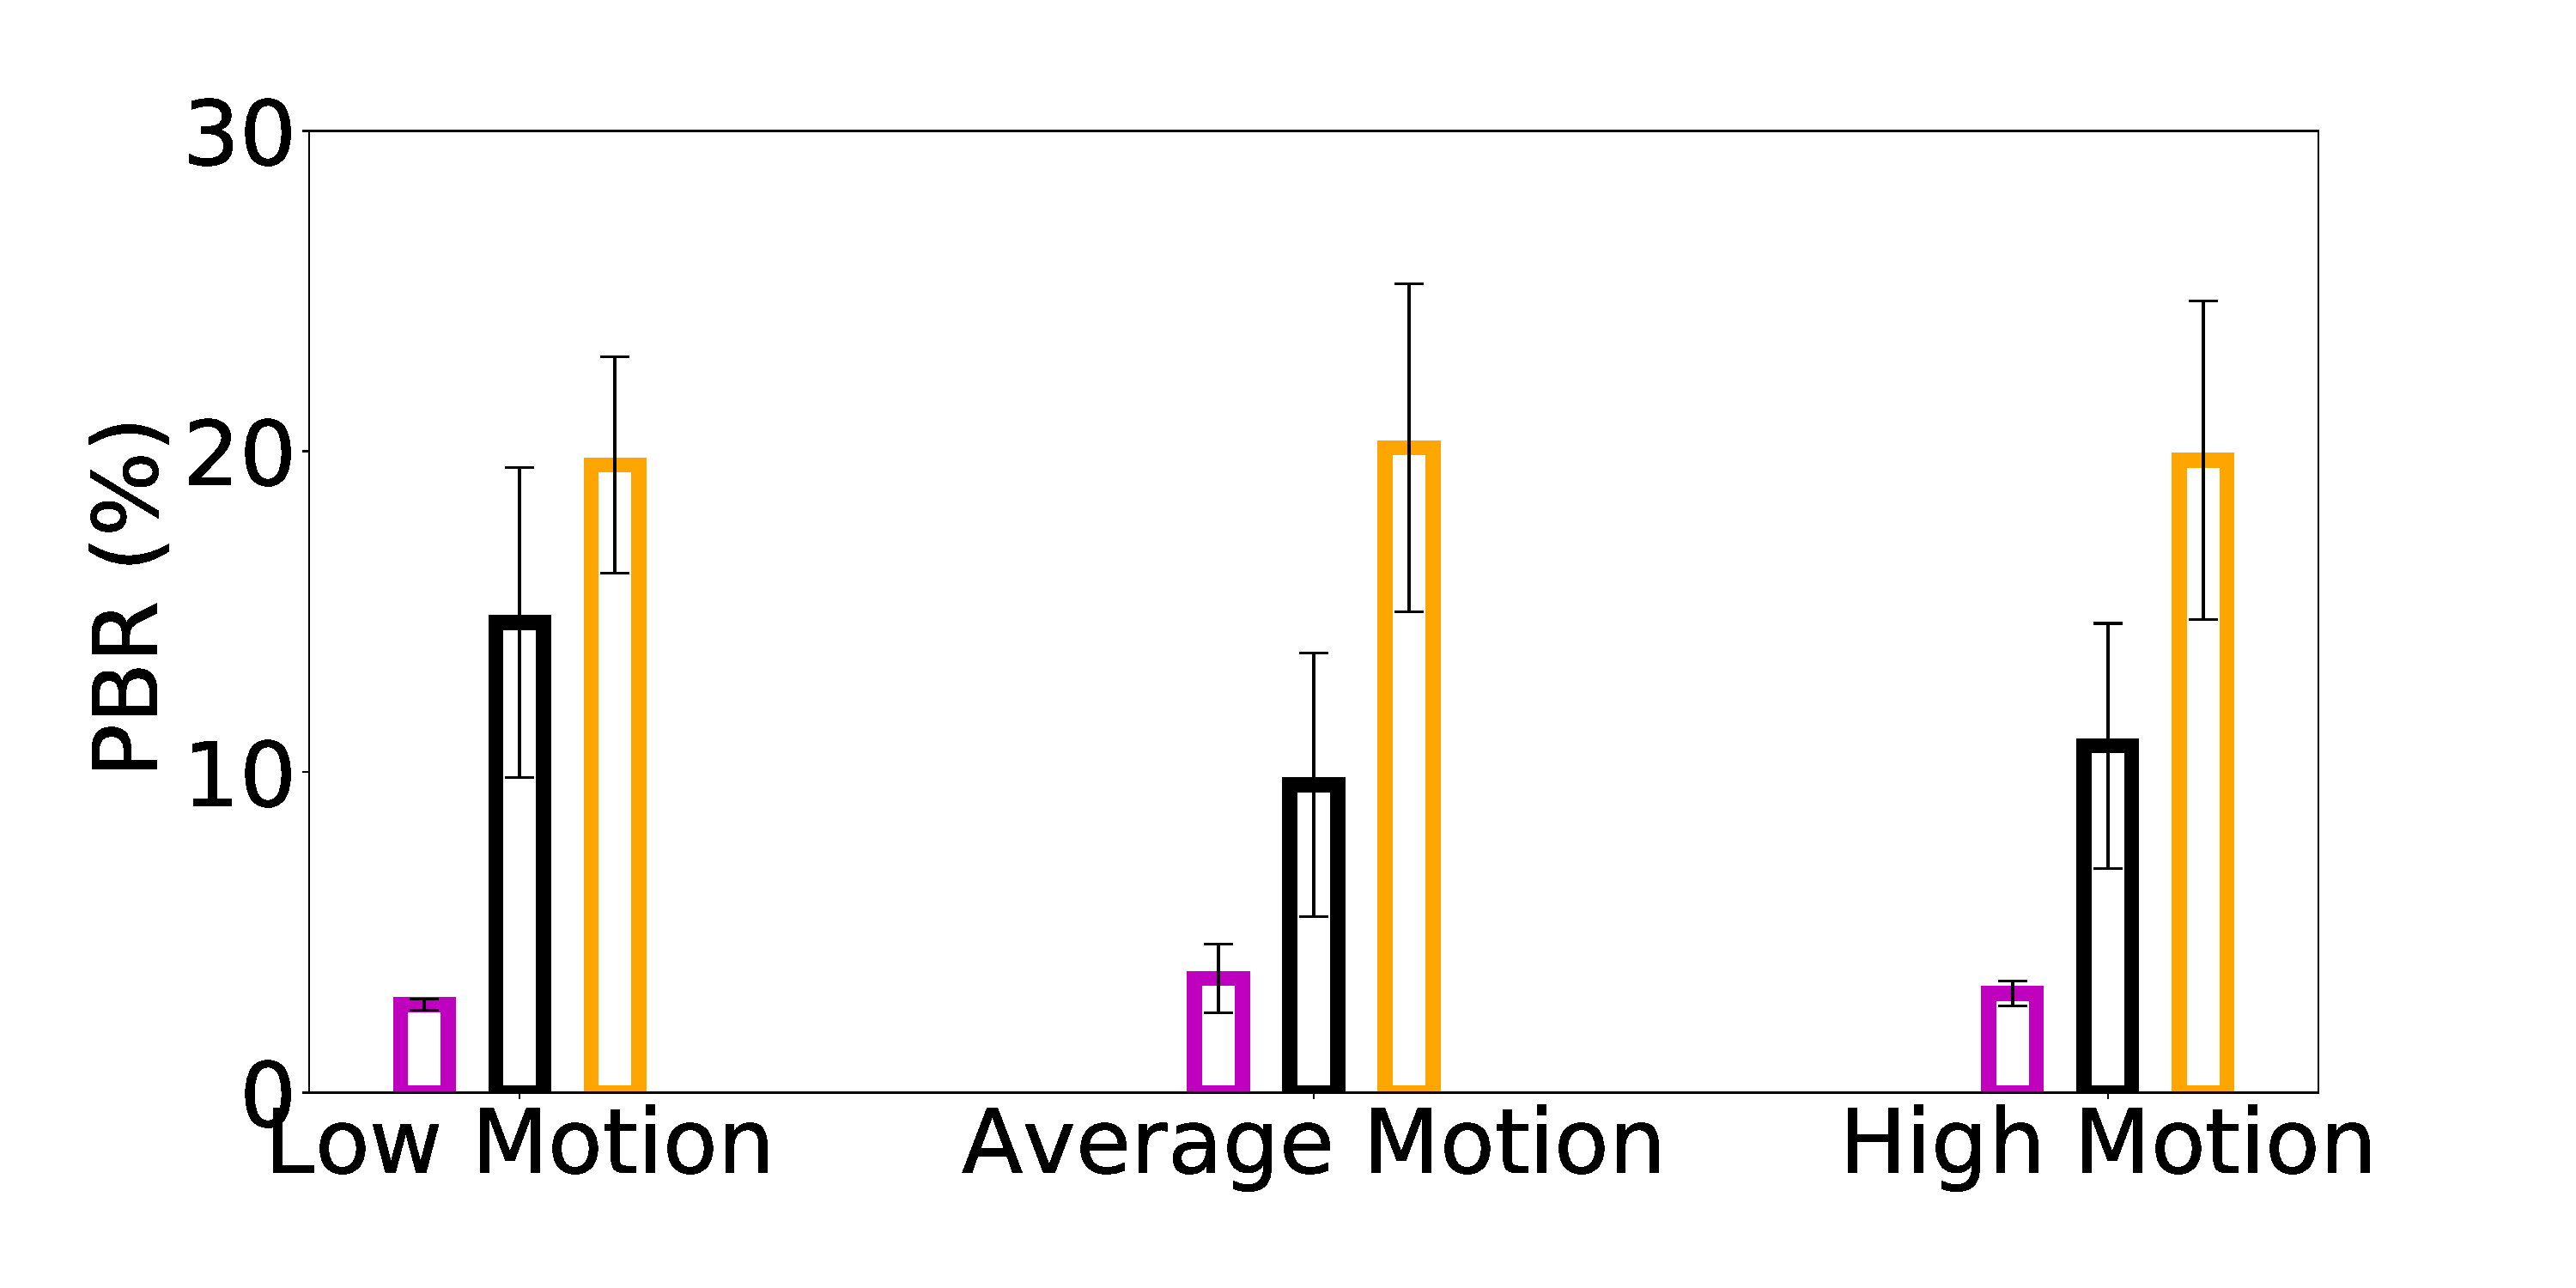
\includegraphics[width=1\linewidth]{sections/network-work/content-bitrate}
        \caption{Content and Motion}
    \end{subfigure}
    \begin{subfigure}[b]{0.33\textwidth}
        \centering
        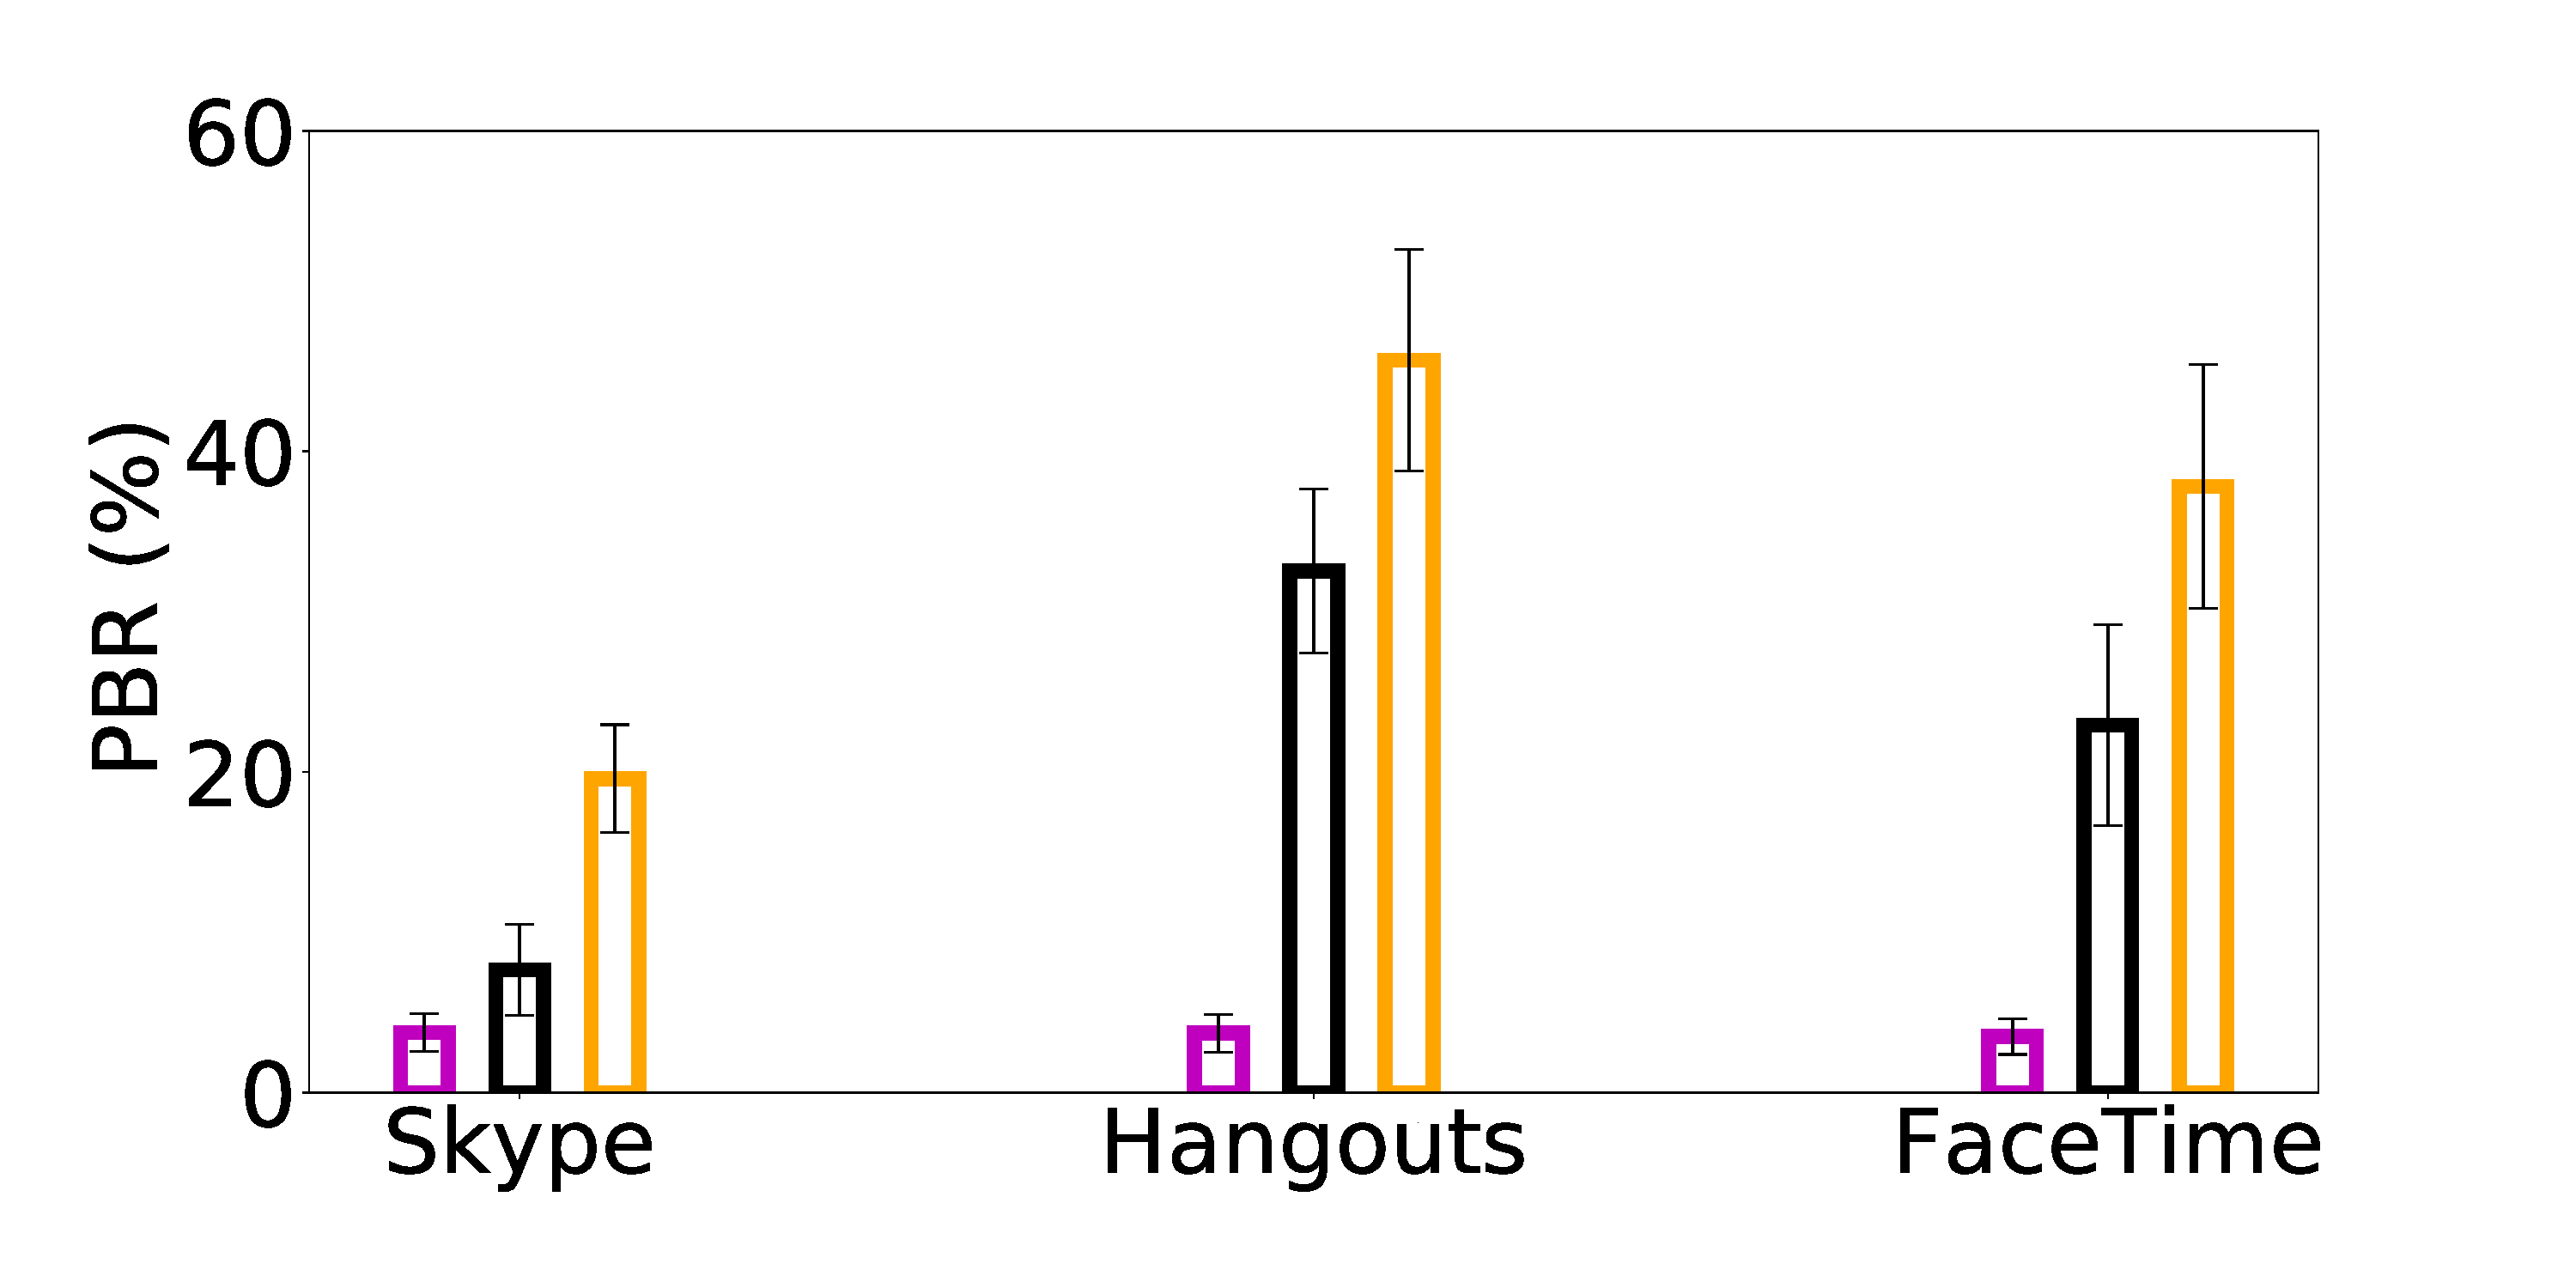
\includegraphics[width=1\linewidth]{sections/network-work/app-bitrate}
        \caption{Applications}
    \end{subfigure}%
    \begin{subfigure}[b]{0.33\textwidth}
        \centering
        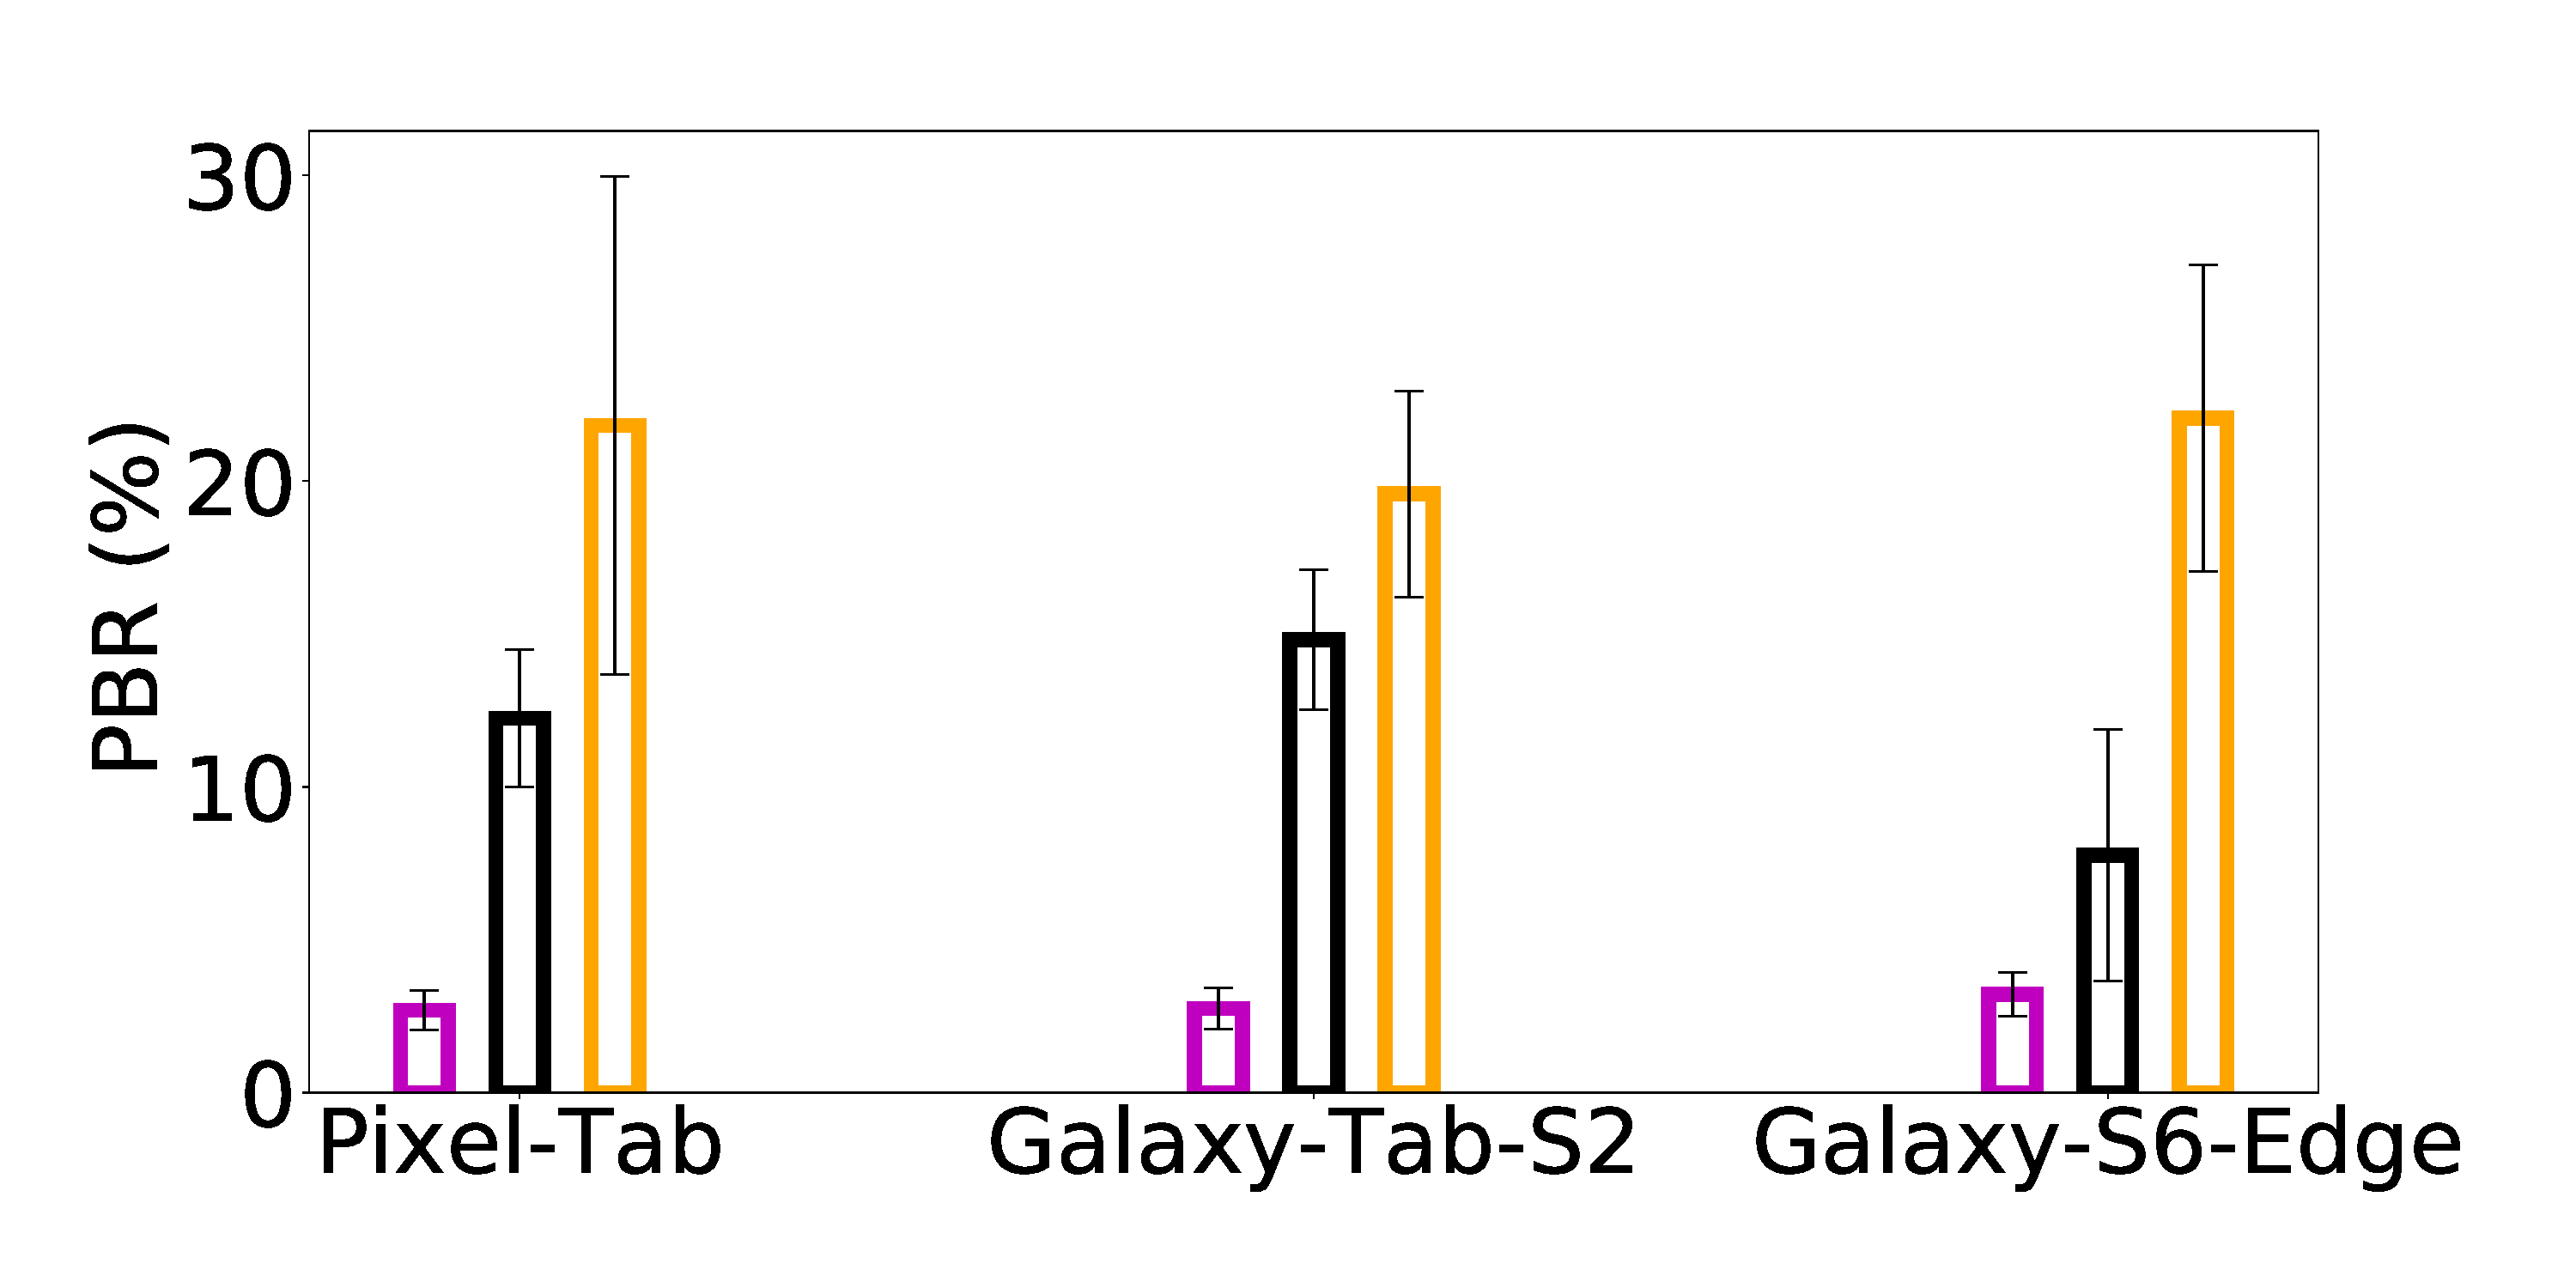
\includegraphics[width=1\linewidth]{sections/network-work/dev-bitrate}
        \caption{Devices}
    \end{subfigure}

     \begin{subfigure}[b]{0.33\textwidth}
        \centering
        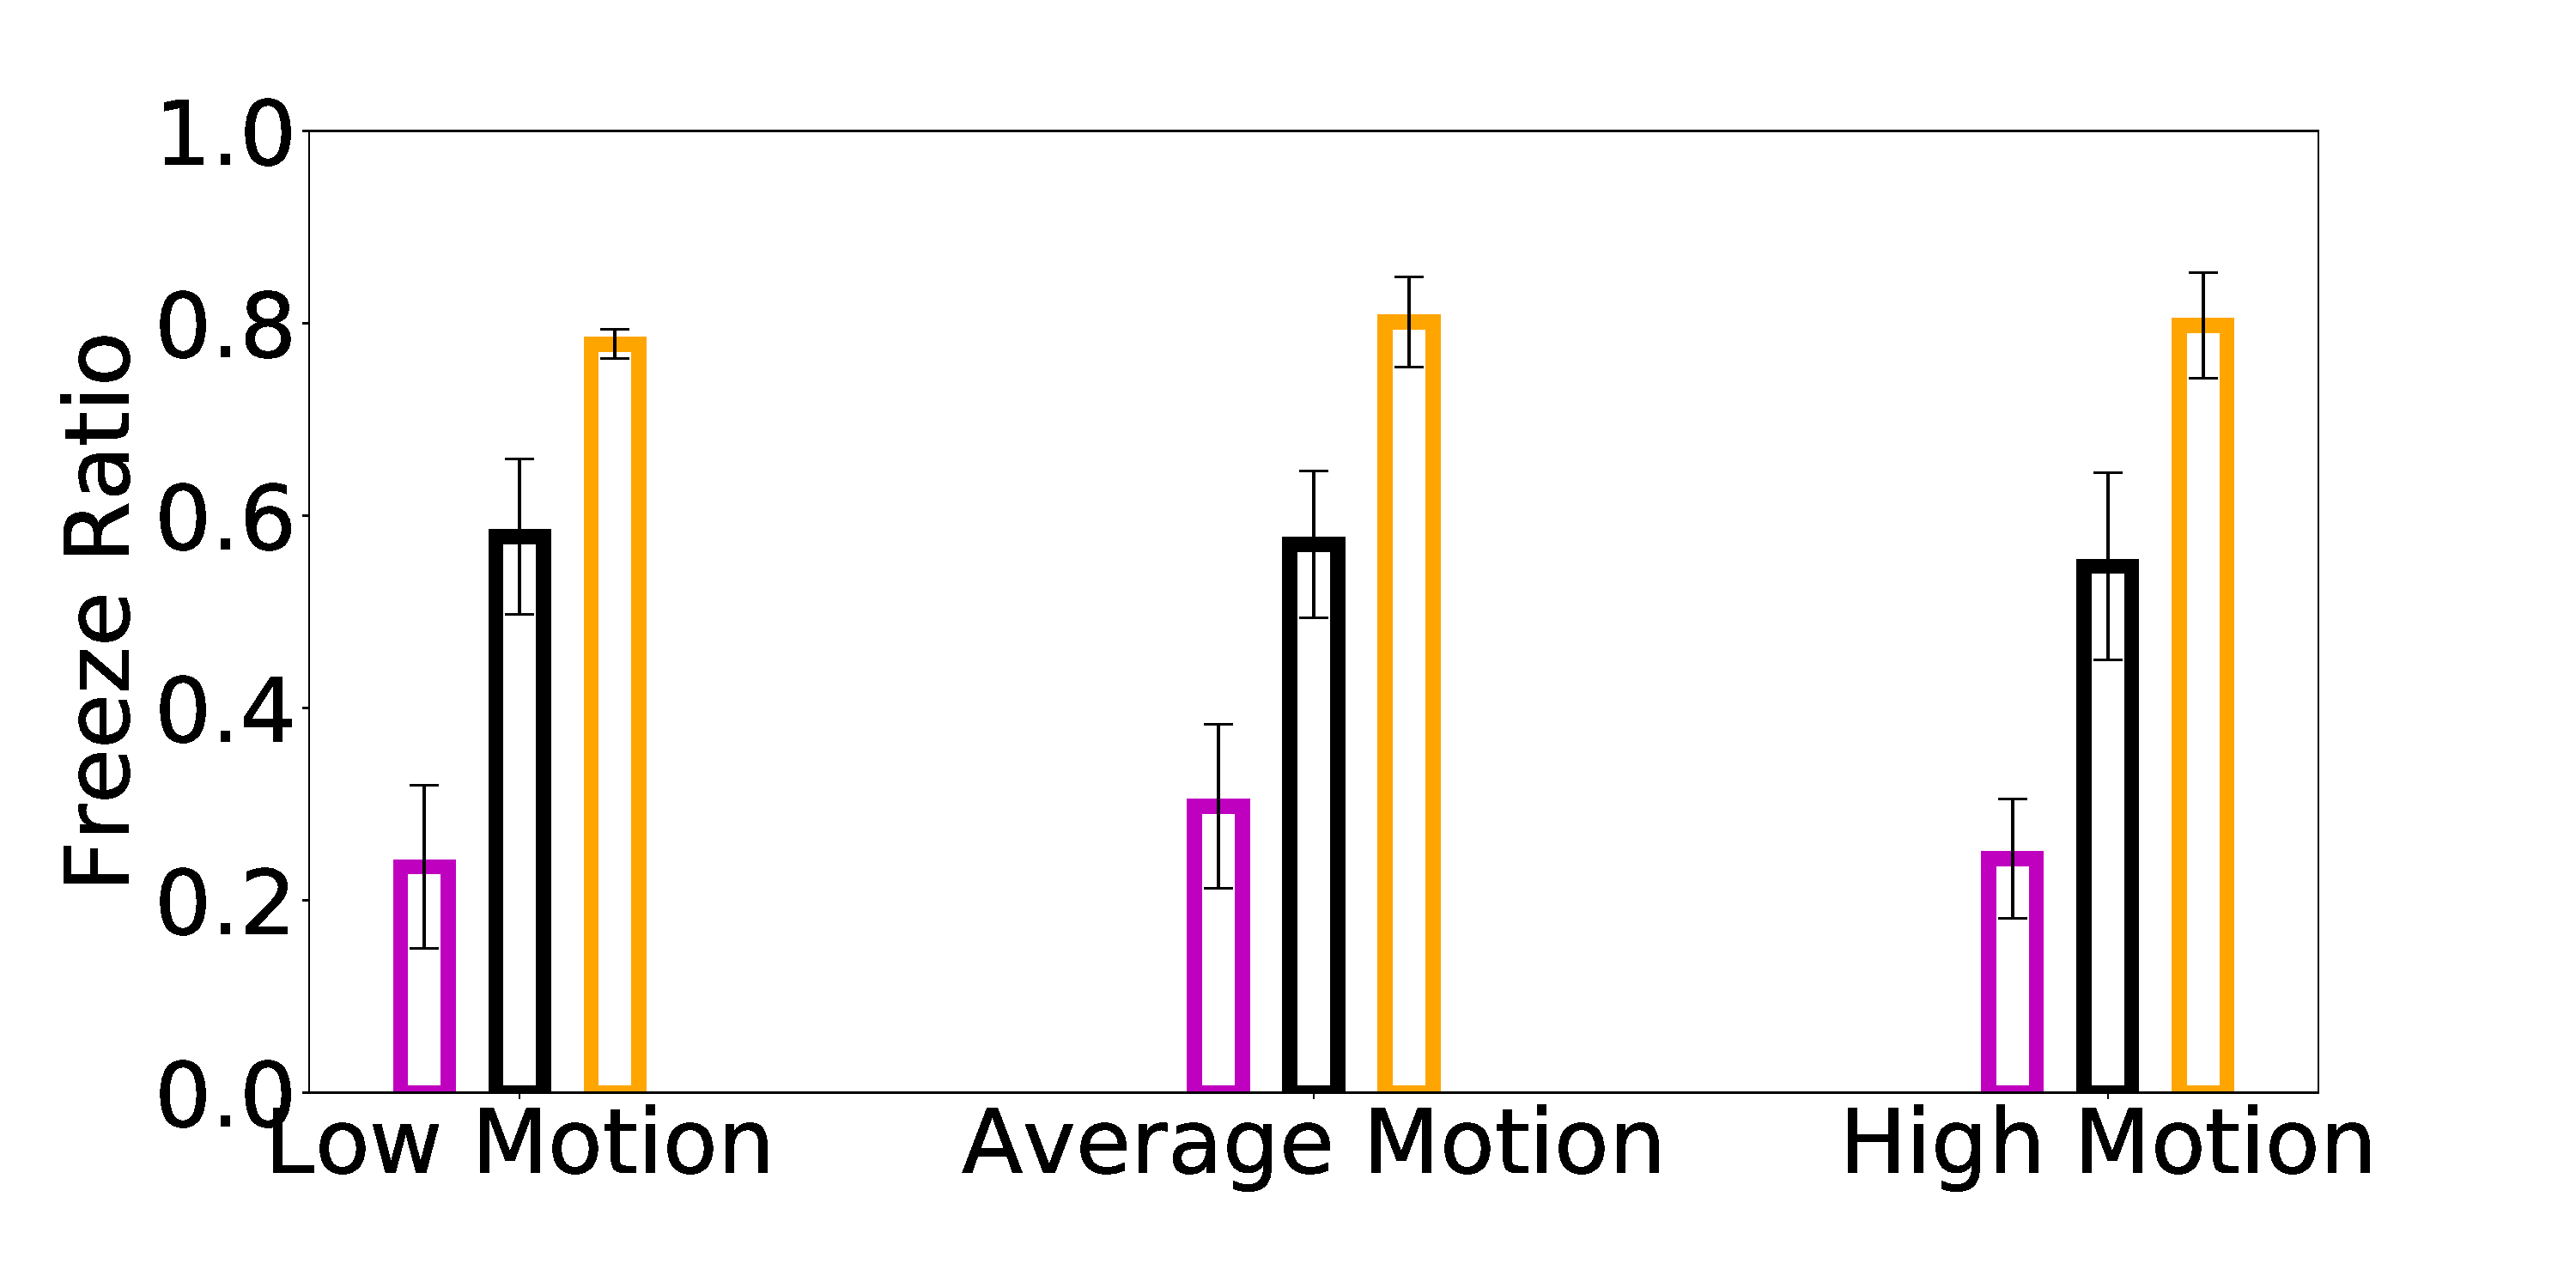
\includegraphics[width=1\linewidth]{sections/network-work/content-stutter}
        \caption{Content and Motion}
    \end{subfigure}
    \begin{subfigure}[b]{0.33\textwidth}
        \centering
        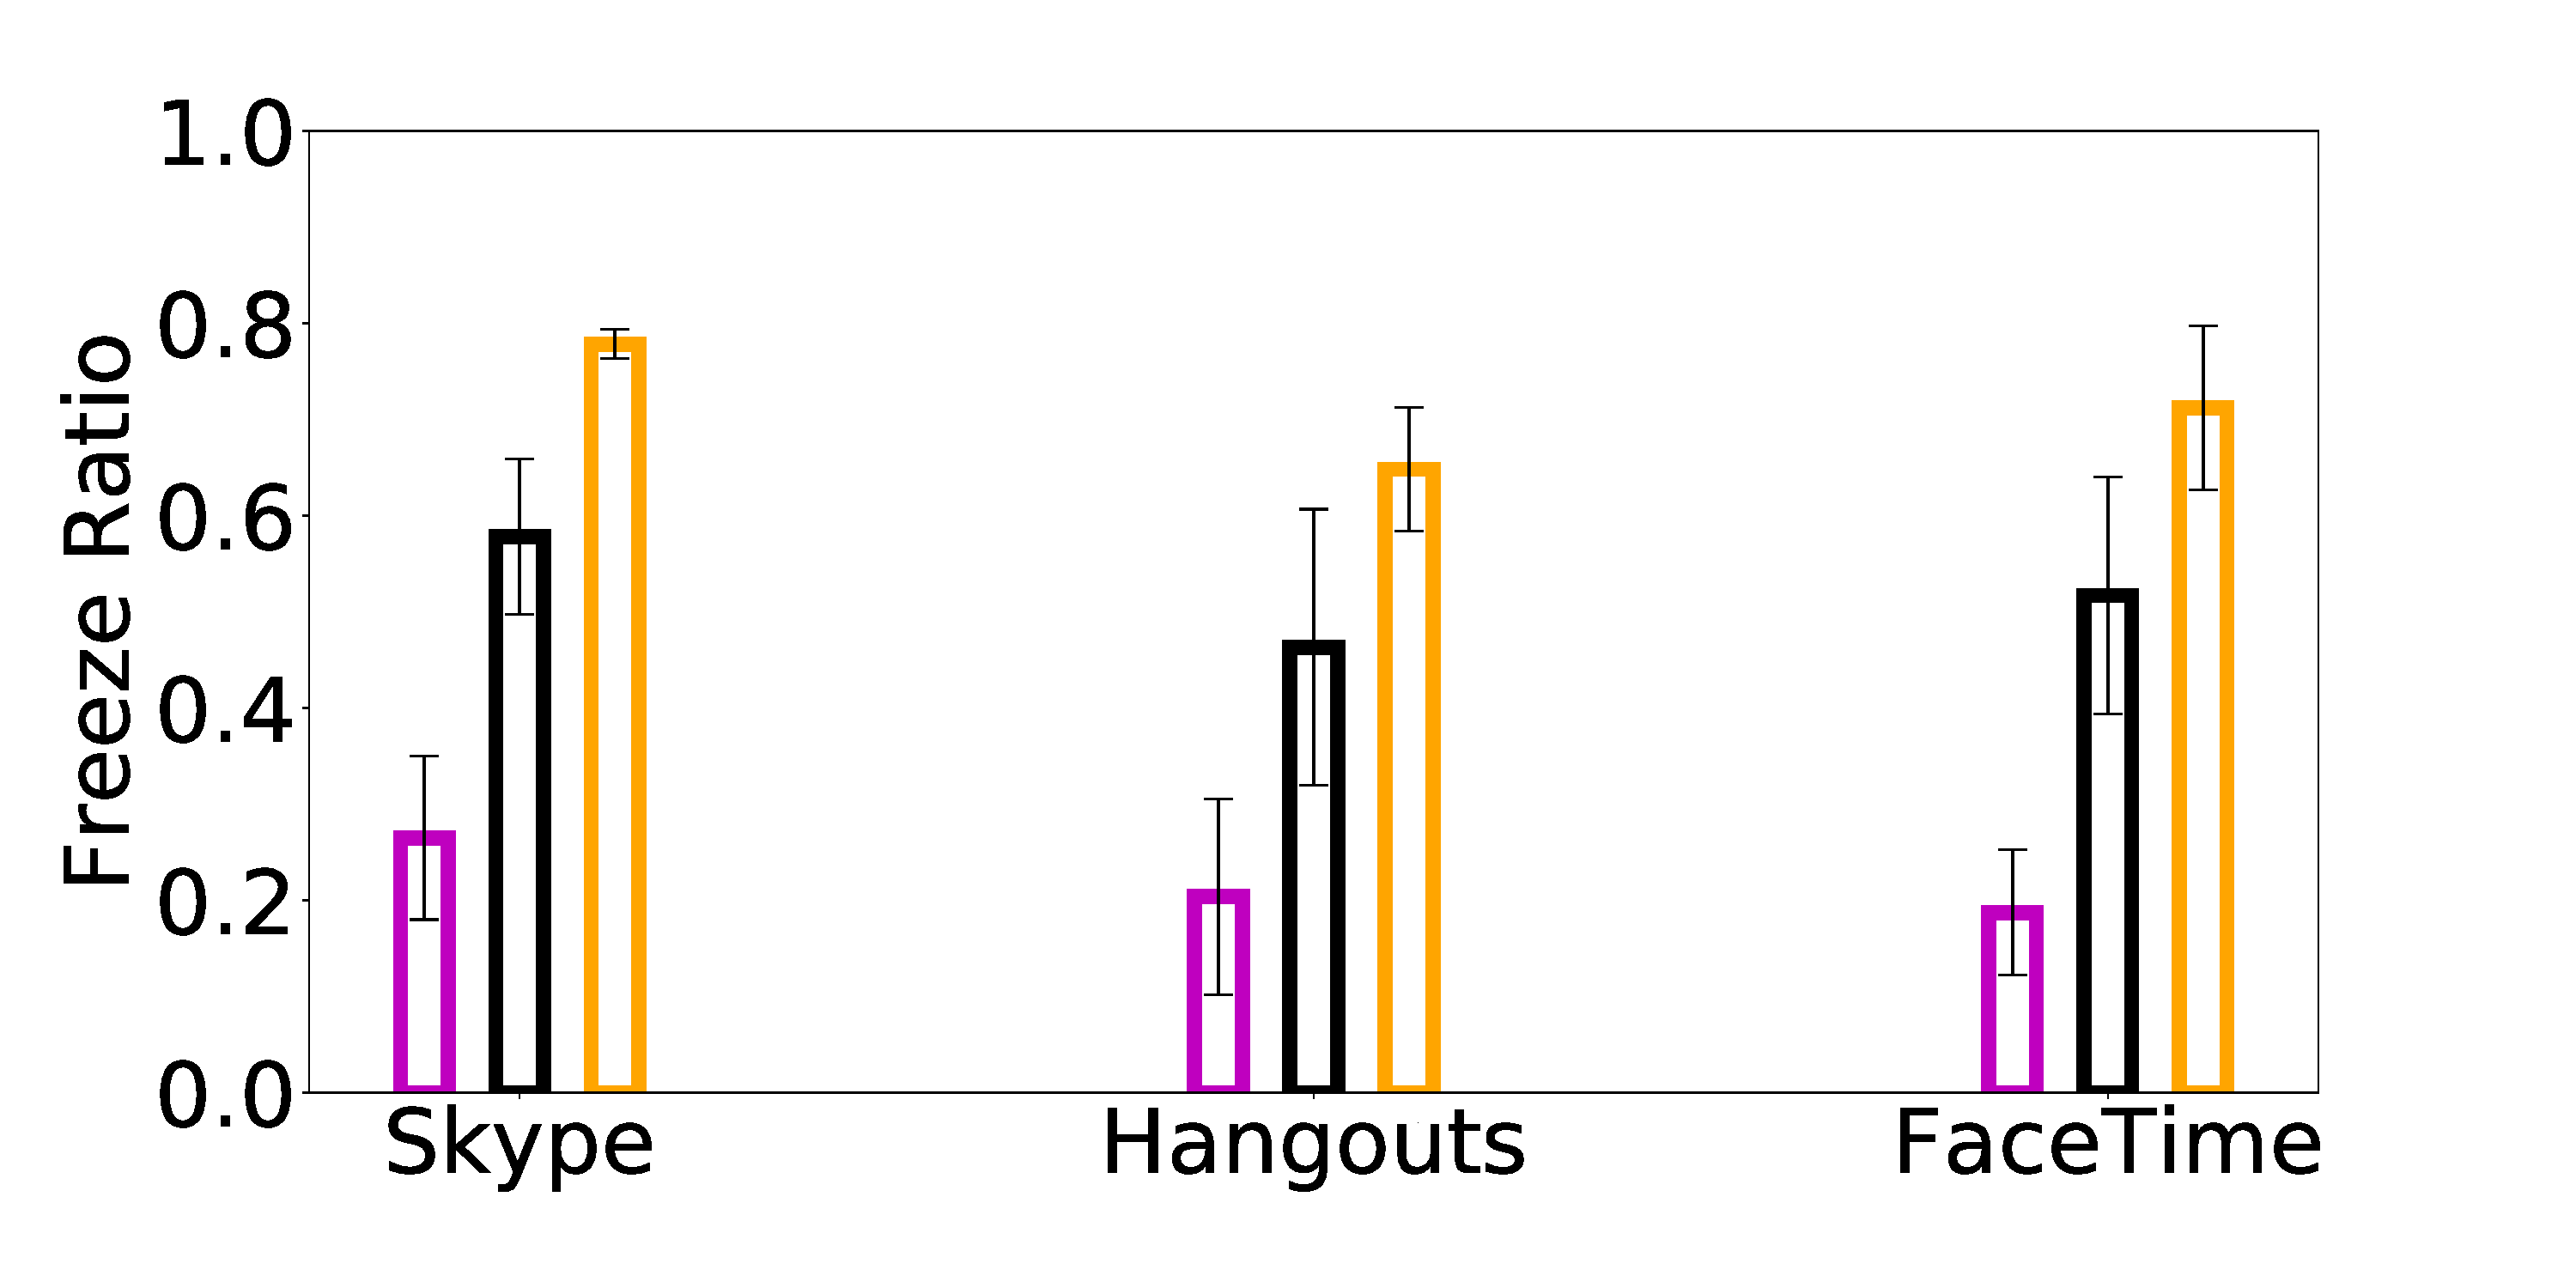
\includegraphics[width=1\linewidth]{sections/network-work/app-stutter}
        \caption{Applications}
    \end{subfigure}%
    \begin{subfigure}[b]{0.33\textwidth}
        \centering
        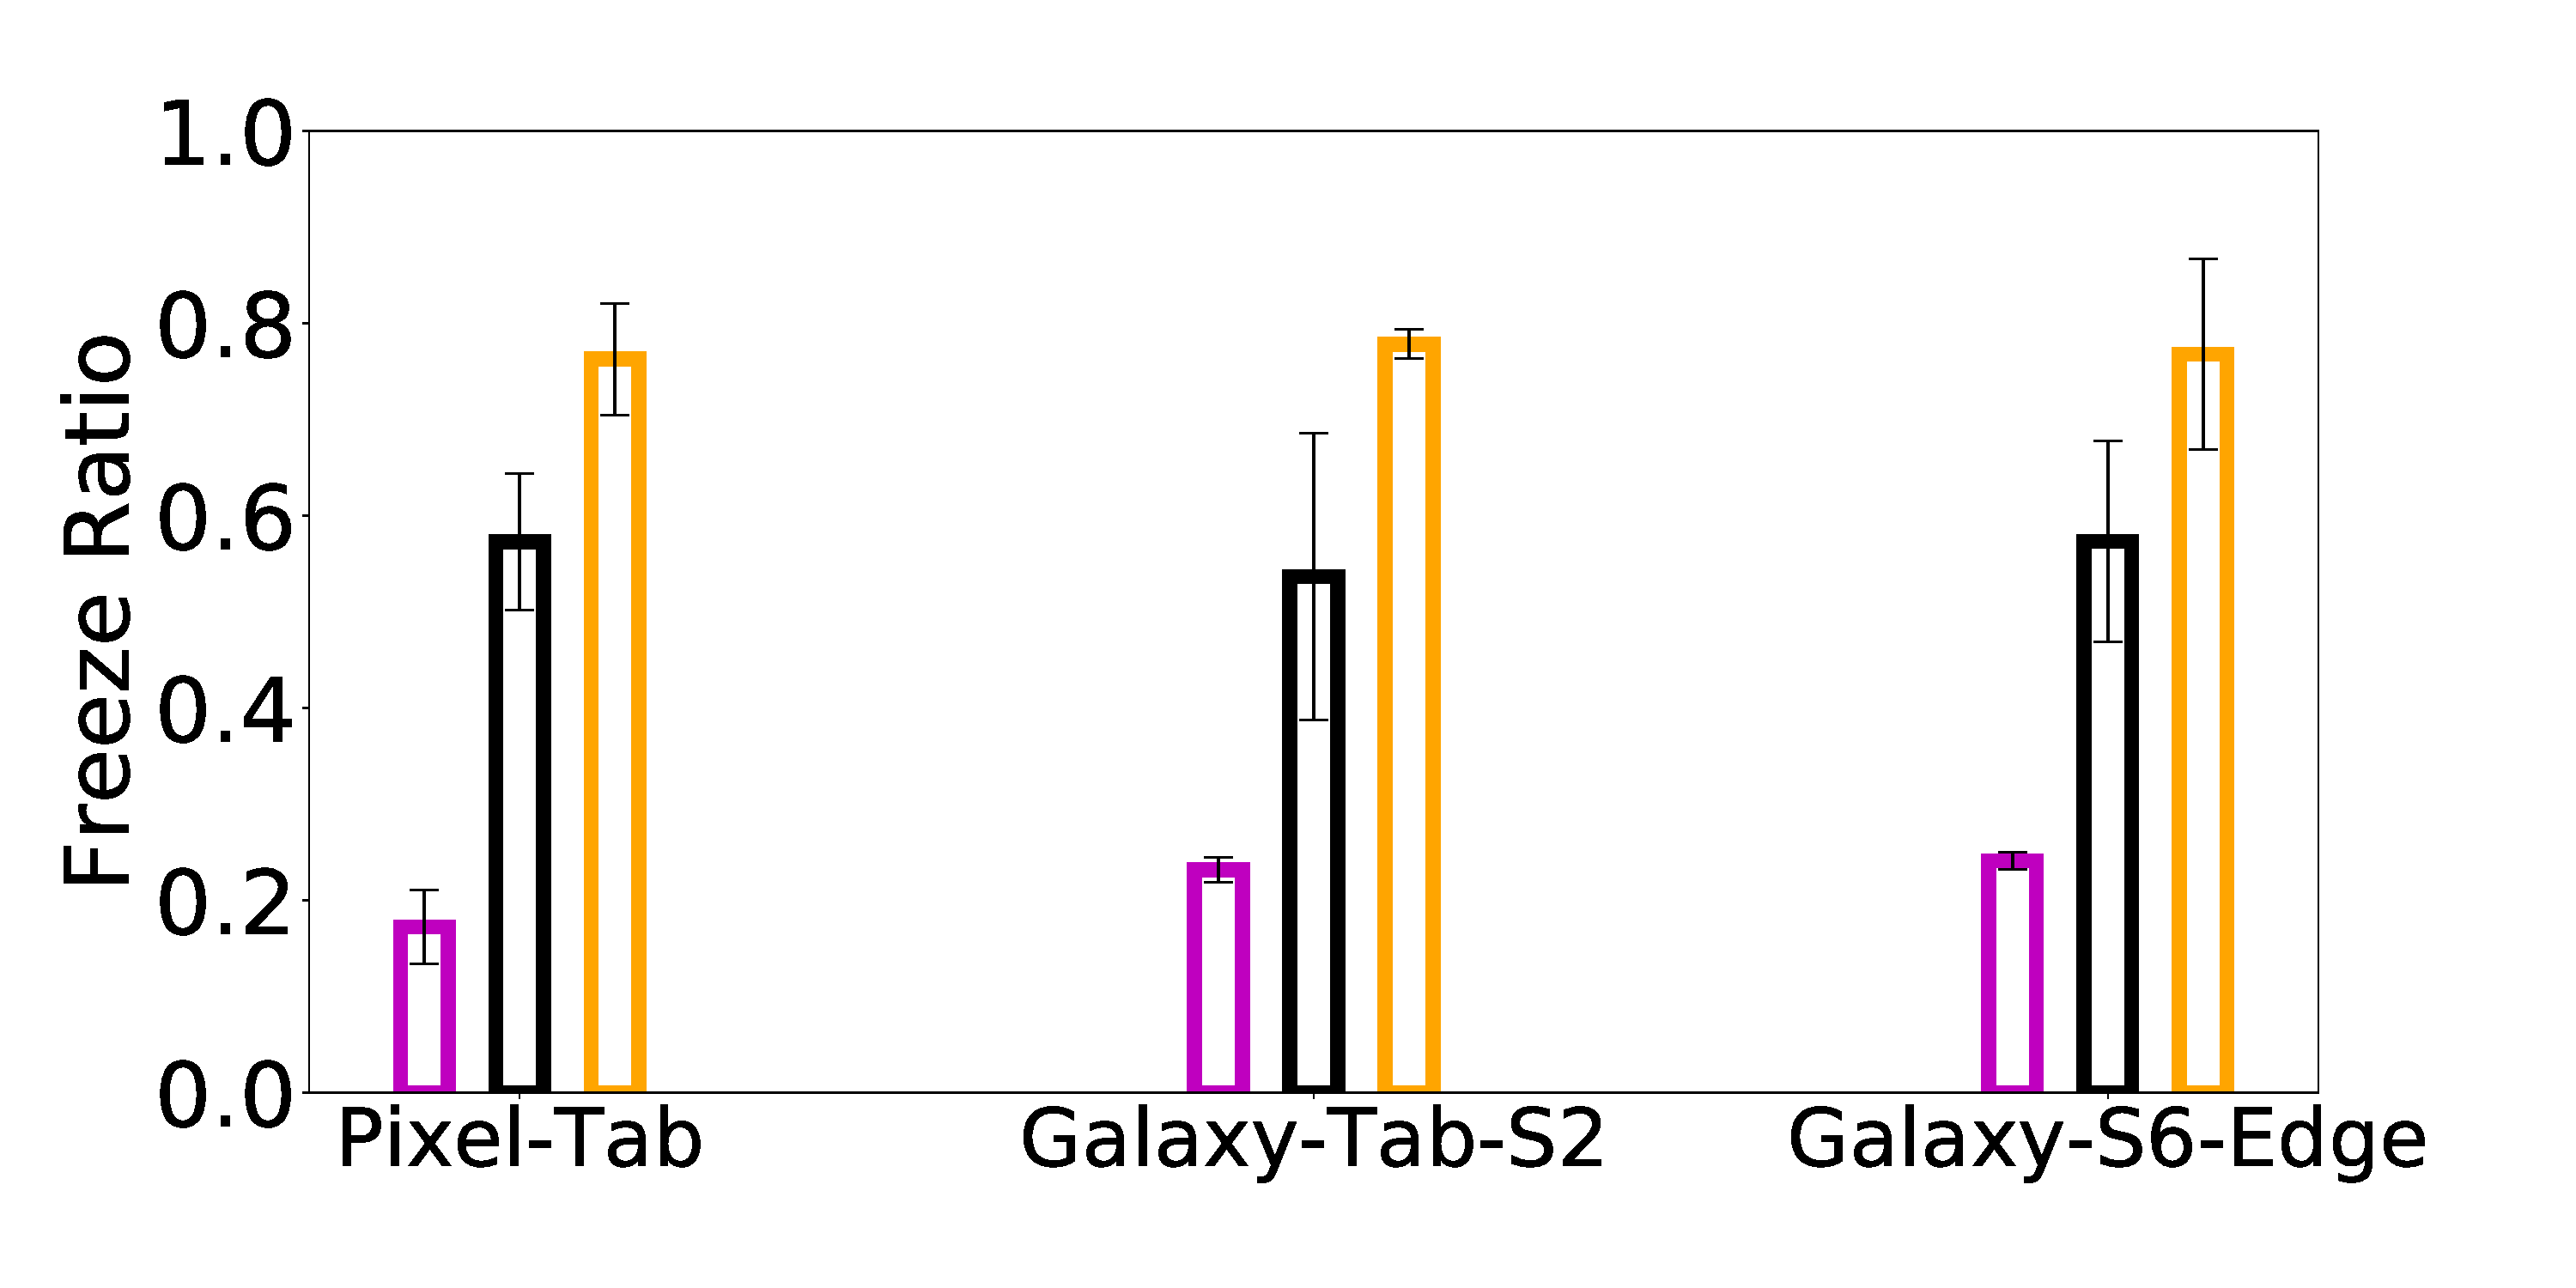
\includegraphics[width=1\linewidth]{sections/network-work/dev-stutter}
        \caption{Devices}
    \end{subfigure}
    \caption{PBR and Freeze Ratio for different videos with respect to content, application and device settings. Results for diverse network conditions are shown (from bad, average, good).}
     \label{fig:measurements}
     \vspace*{-1em}
\end{figure*}

\noindent \textbf{Network conditions:} As we experiment real-time with interactive applications (Skype, Hangouts, FaceTime), we need to emulate real user experience under any condition and to obtain samples with MOS values of all levels (1--5). Hence, we conduct tests with ideal network conditions and with throttled network. To create average and bad network conditions, we use Linux utility \texttt{tc} and we introduce hundreds of ms of delay, packet loss (10--20\% ensuring that the call is setup), or low bandwidth (2--10 Mbps).  

\noindent \textbf{Test video sequences:} We use the same 20 test video sequences as in Section \ref{MOTIVATION}. 
We collect these videos  from Xiph media \cite{xiph2008org} and YouTube. We select 20 representative videos that contain different types of motion and content.
All videos are downloaded in Full HD (1920x1280) resolution.
%Our automated Telephony client is restricted to few container formats, so we could not host raw videos but had to encode into AVI container format. 
%While converting $y4m$ into $AVI$, we use $ffmpeg$ to extract $fps$ and $bitrate$ of compression. We exploit these video coding artifacts in classifying the motion present in the video. We observe motion is directly proportional to $fps$ and inversely proportional to output $bitrate$ of video coding. Table~\ref{tab:table2} gives statistics corresponding to motion in the video. All the videos are of High Definition (HD ) resolution with $16:9$ aspect ratio and $4:4:4$ color space format. The videos are encoded under same encoding parameters such as libx264 video codec, quantization parameter (25), YUV $4:2:0$ output color space format.

\subsection{Our QoE Metrics}
%In this section, we describe our QoE metrics.

\noindent \noindent \textbf{PBR:} 
Video bitrate has been considered a standard metric for perceptual quality of video \cite{zhang2012profiling, chakraborty2016exbox}.
We compute the bitrate of recorded videos as a QoE metric. Typically, the bitrate is lower for low resolution video and higher for high resolution video and depends on the level of video compression.
Therefore, we capture video blur with \texttt{encoded bitrate} by compressing the recorded video. 
We employ the observation that the blurrier the video is, the higher compression efficiency is. 
However, we find that the bitrate metric is sensitive to motion in the video, because the block movement for high motion videos is very high and it is low for low motion videos. This results in different encoding bitrates. 
As described in Section \ref{label:background}, low motion videos take advantage of inter-frame prediction, which makes the encoded bitrate motion-sensitive. 
Therefore, we use intra-coded bitrate by \emph{disabling the inter frame prediction while compressing video.}
We experiment with different encoding parameters like quantization parameter (QP) and de-blocking filter techniques and we choose high QP value (30) while coding, to get large bitrate difference when encoding high- and low-quality videos. 
To achieve robustness to video content, we compute the \emph{relative change between the recorded bitrate and  the intra-coded bitrate of the compressed video.} We define this change as the perceptual bitrate (PBR), as it only captures quality of the image. Since we calculate PBR on the recorded video, we do not need a reference video, hence PBR is a no-reference metric.

We validate the PBR metric with respect to the same 20 videos used to compute blur using DCT coefficients in Section \ref{MOTIVATION}.
We create two sets of videos with high and low quality and record them during a Skype call under best network conditions.
This experiment aims to validate our blur capturing metric, hence we avoid video freezes by sending low quality videos over best network conditions.
Fig. \ref{fig:ourblurdetection} shows PBR for both low and high quality videos.
We observe a PBR larger than 20\% for low quality videos, whereas PBR is smaller than 5\%  for high quality videos.
Unlike blur detection using previous methods, we see a clean separation of average PBR between low and high quality videos. Therefore, PBR can be used to detect blurriness in videos without any ambiguity.

%In addition to PBR, we also compute gradient of PBR (PBR-G). This denotes the number of times the quality level is changed in a given video call. This variation happens because of adaptive video-streaming solutions. More specifically, the clients estimate the bandwidth and request corresponding video quality from server. If the network conditions change frequently, quality of video also fluctuates frequently. Because of this high variability in quality, the users get dissatisfied easily. Therefore, we use \texttt{PBR} and \texttt{PBR-G} metrics to capture spatial artefacts of QoE.

\noindent \textbf{Freeze Ratio:} As described in Section \ref{label:background}, freeze ratio is another important QoE artefact. 
Freeze ratio is the number of repeated frames over total frames in a given window, i.e., it denotes the amount of time the video is paused because of network disturbance. 
We use Ffmpeg's \textit{mpdecimate} \cite{ffmpeg} filter in calculating freeze ratio. 
The \textit{mpdecimate} algorithm works as follows: The filter divides the current and previous frame into 8x8 pixels blocks  and computes sum of absolute differences (SAD) for each block. 
A set of thresholds (\textit{hi, lo and frac}) are used to determine if the frames are duplicate. 
The thresholds \textit{hi} and \textit{lo} represent number of 8x8 pixel differences, so a threshold of 64 means 1 unit of difference for every pixel. A
frame is considered to be duplicate frame if none of the 8x8 blocks yields SAD greater than a threshold of \textit{hi}, and if no more than \textit{frac} blocks have changed by more than \textit{lo} threshold value. 
We experiment with several other error methods such as MSE and MAD, but we notice similar results among all three, thus we choose SAD for minimal computation overhead. 
We use threshold values of 64*12 for \textit{hi}, 64*5 for \textit{lo} and 0.1 for \textit{frac} for all our experiments. 
The metric does not work if the entire video is having a still image (for instance a black screen throughout the video). 
However, we think that it is a reasonable assumption that most of video telephony applications do not generate such video content.

In addition to freeze ratio, we also compute length and number freezes in video. We define a freeze if the video is stalled for more than one second. We observe that users do not perceive the stall when the length of freeze is very short or if there are very few such short freezes in the video. Therefore, we employ \texttt{freeze ratio, length and number of freezes} metrics to capture the temporal artefacts of QoE.

\subsection{Micro-Benchmarking of Video Artefacts}
In this section, we show the scalability of our metrics through measurements across different applications and devices. As described above, we use a total of 4 metrics: PBR, freeze ratio, length and number of freezes in the video. For brevity, we show measurements for only PBR and freeze ratio. We find similar trends with other metrics as well. We measure these metrics with 6 different videos from the 20 videos described in Section \ref{MOTIVATION}, that cover high video-motion and content diversity. These experiments are run on Skype and Samsung Galaxy Tab S2 unless otherwise specified. All videos are recorded under Full HD (1920x1280) resolution with 60 Fps. Each experiment consists of 20 minutes video call with a total of 18 hours of video recordings. The videos are recorded under different network conditions to obtain different video quality  levels. We use the following network conditions: good case (0\% loss, 0 latency and 100 Mbps bandwidth), average case (5\% loss, 100 ms and 1 Mbps bandwidth) and bad case (20\% loss, 200 ms, and 512 Kbps bandwidth). Fig. \ref{fig:measurements} shows PBR and freeze ratio across different applications and devices. Our observations are the following.



\noindent \textbf{Video Motion and Content Diversity:} 
The average PBR for best network conditions is always smaller than 5\%. PBR is larger than 20\% under bad settings (see In Fig.~\ref{fig:cont-pbr}). 
The average freeze ratio for best network conditions is smaller than 0.3 and for bad conditions, it is larger than 0.8 (Fig.~\ref{fig:cont-st}). 
We observe that both PBR and freeze ratio are highly impacted by network conditions and follow same trend with network quality irrespective of content and motion in the video.
Therefore, the videos can be labeled accurately because of clear separation between network dynamics.

\noindent \textbf{Application Diversity:} 
In Fig.~\ref{fig:app-pbr},~\ref{fig:app-st}, we present PBR and freeze ratio for three applications: Skype, FaceTime and Hangouts.
For Skype, we observe an average PBR of less than 5\% with good network and 20\% with bad network. 
Whereas, both FaceTime and Hangouts reach more than 40\% PBR under bad network. 
This discrepancy is due to application logic: Skype does not compromise quality of video, hence low PBR. But, this causes Skype video calls to be stalled more frequently compared to other applications under bad network scenarios. Whereas,  bitrate adaptation of FaceTime and Hangouts sacrifices quality to provide temporally smooth video. 
Moreover, quality and bitrate are highly impacted by the underlying video codec the application uses. In our experiments, Skype uses H.264 whereas Hangouts uses VP8. We observe that using different video codecs and adaptive bitrate (ABR) algorithms impacts video quality during call.

The freeze ratio for Skype is similar to FaceTime and Hangouts. However, as network conditions worsen, Skype yields more freezes compared to other applications. Despite the additional freezes, the average freeze-ratio for Skype is only 0.1 larger than other applications. This is due to the longer freezes of FaceTime and Hangouts than of Skype.

\noindent \textbf{Device Diversity:} We aim to devise a model that is independent of the device that runs video telephony. Our metrics should capture similar video QoE on different devices given that screen recorder and network conditions are the same. To this end, we evaluate our metrics on three devices: Samsung Galaxy Tab S2, Samsung Galaxy Edge S6 and Google Pixel Tab. 
In Fig.~\ref{fig:dev-st},~\ref{fig:dev-pbr}, we observe that both PBR and freeze ratio show same distribution under different network settings on all devices. Hence, our metrics are device independent.

\begin{figure*}[t]
  \centering
  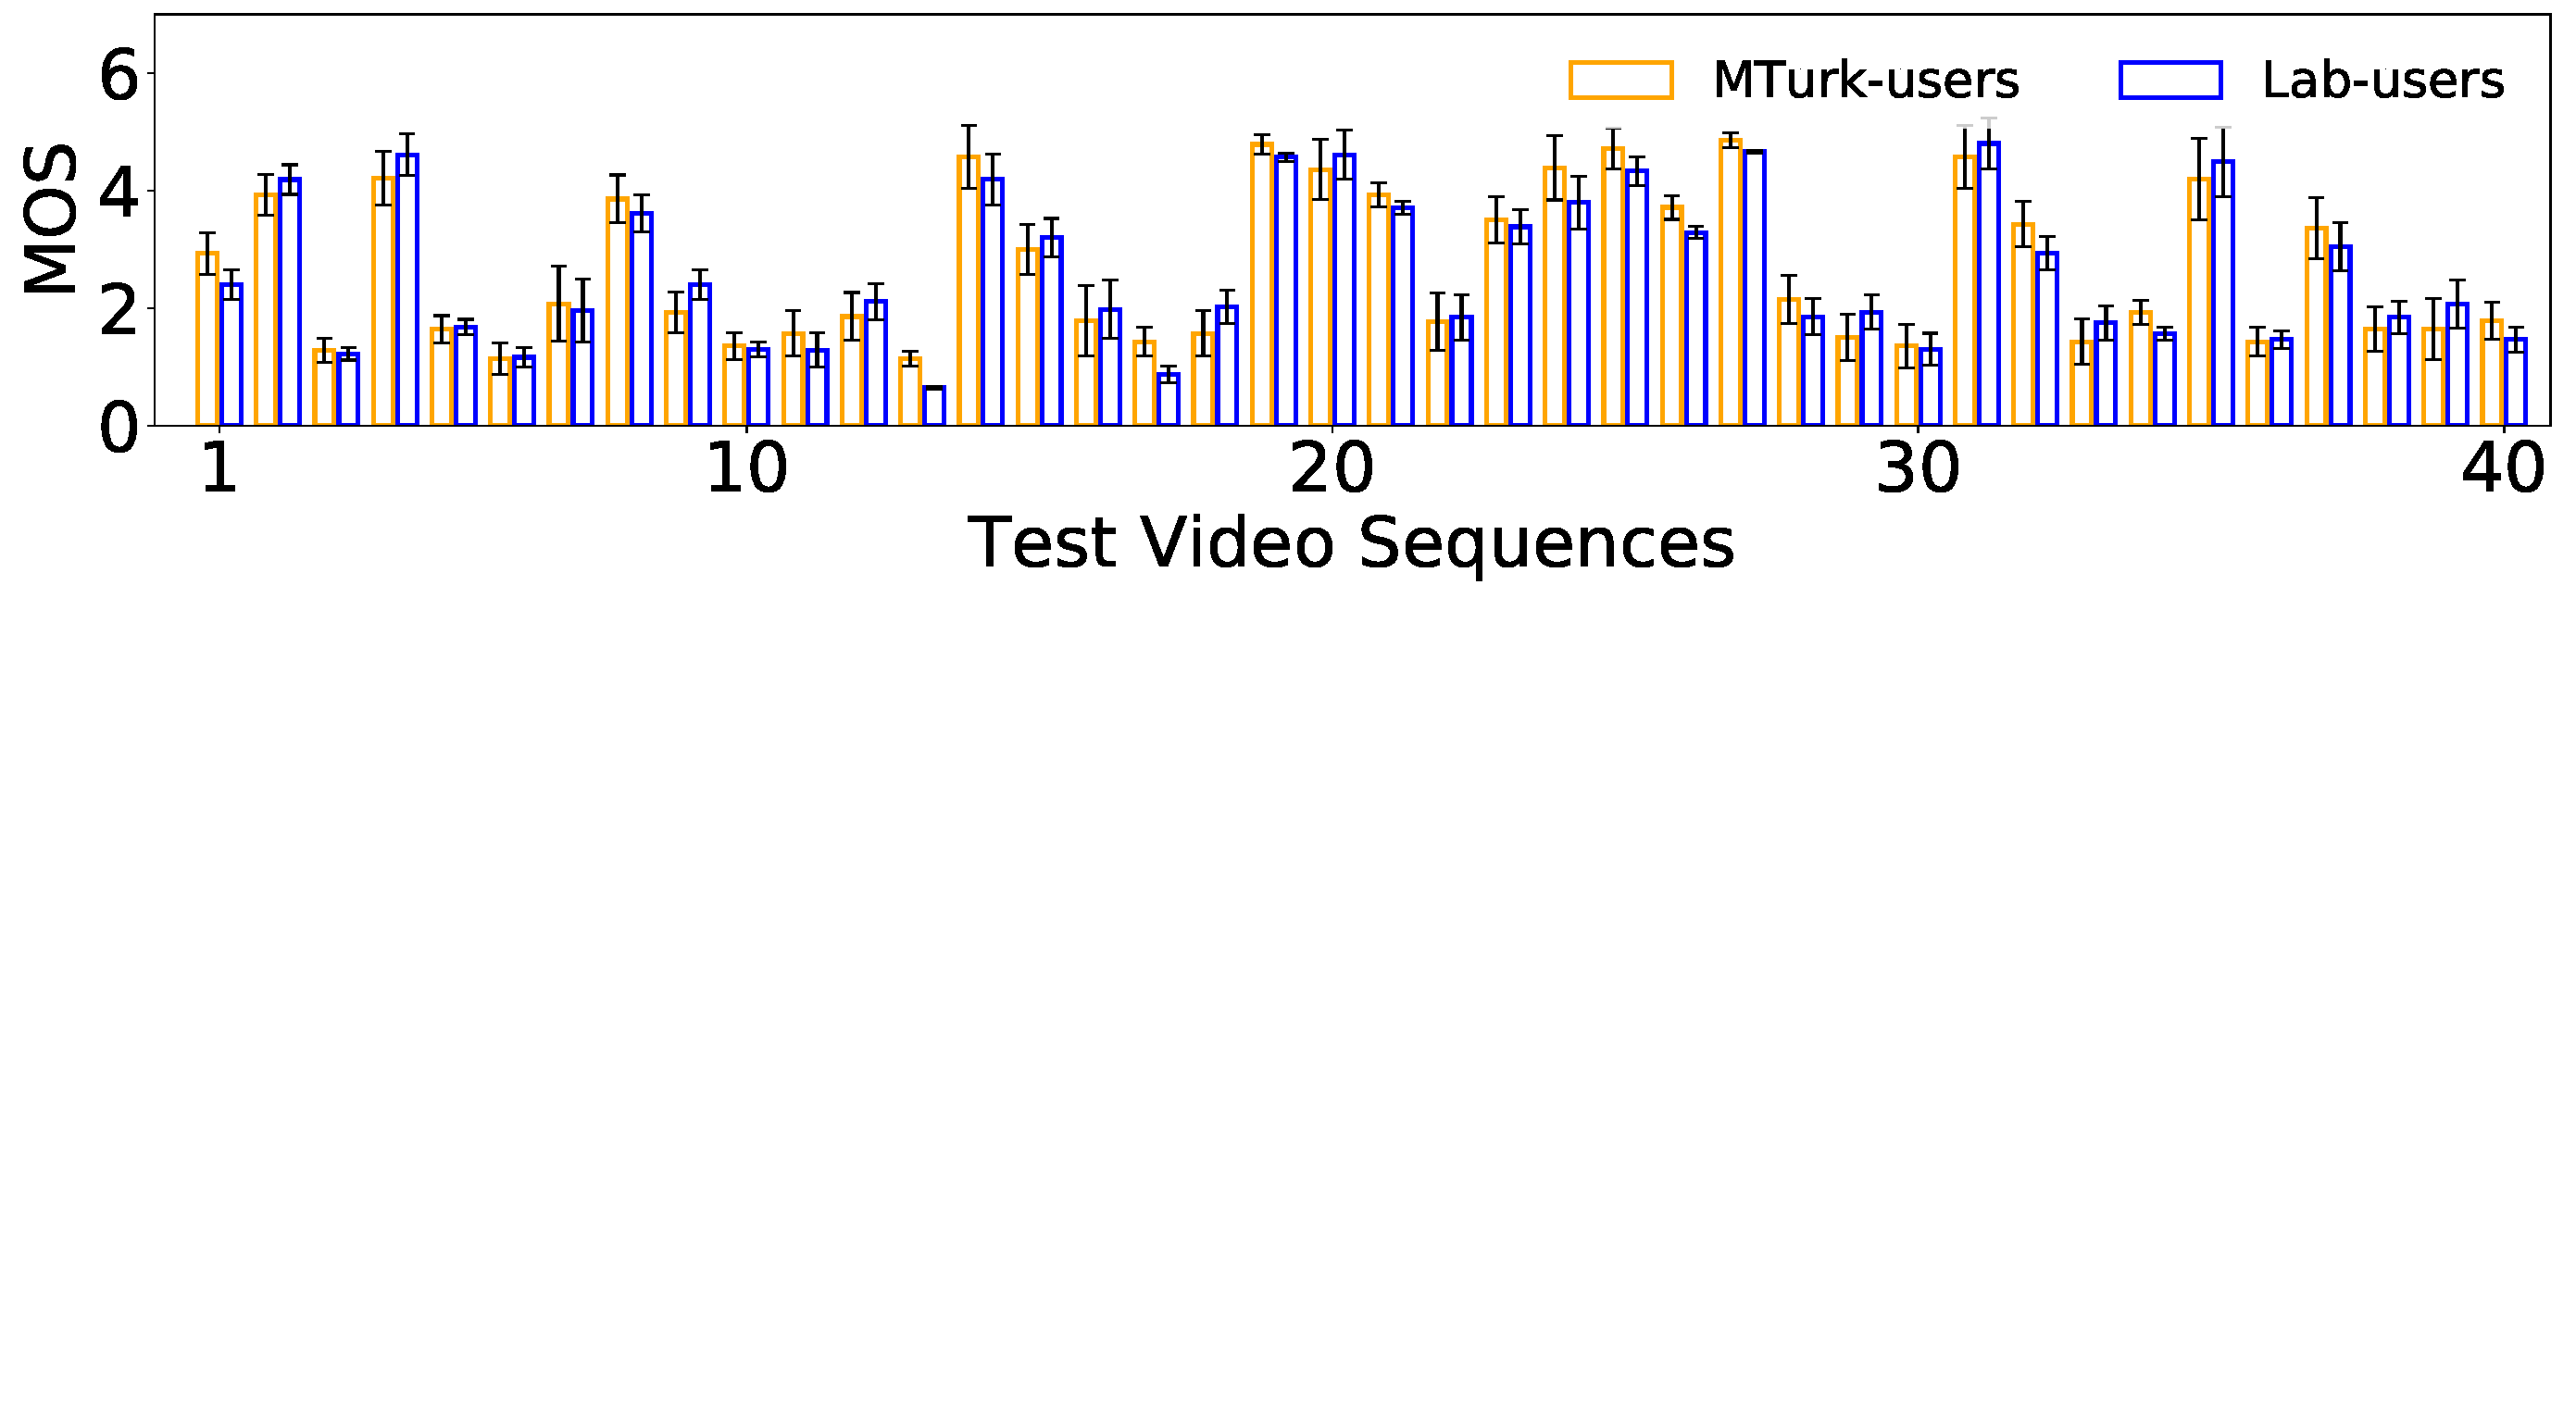
\includegraphics[width=0.8\textwidth]{sections/network-work/mos}
  \vspace{-2in}
  \caption{MOS and standard deviation of QoE scores from 30 lab and 30 online users. Although the scores vary across the users both in lab and online, the distribution of MOS is similar in two cases.}
  \vspace{-0.15in}
  \label{fig:mos}
\end{figure*}

\section{From Video Artefacts to Q\lowercase{o}E} \label{label:results}
We validate our QoE metrics presented in Section~\ref{label:design} with subjective measurements. We seek to ensure that our metrics accurately capture  video telephony QoE artefacts. Video artefacts vary across applications and network conditions. Additionally, they can appear together (e.g., when we have both blurriness and stutter) or independently. Intermingled video artefacts result in diverse QoE levels (from bad to excellent), standardized as MOS by ITU-T~\cite{series2012methodology}\footnote{MOS takes values from 1 to 5, with 5 being excellent.}. We carry out a user study and obtain a MOS for each video.

\subsection{Data Preparation}
As described in Section \ref{label:design}, the dataset is prepared from recorded video calls. We use 20 videos described in Section \ref{MOTIVATION}, for video calls on Skype, FaceTime and Hangouts. For each video and application, we repeat  experiments on  multiple devices. The video calls are recorded under different network conditions to produce good, average and bad quality videos. We record video calls for Skype, Hangouts on Samsung Galaxy (SG) S6 edge, Google Pixel Tab, SG S2 Tab and for FaceTime on iPad Pro (model A1674) and iPhone 8 Plus. We post-process these videos into 30 seconds  video clips and evaluate QoE for each clip. We host a web server with these video clips and ask the users to rate their experience after watching each sample. 

\subsection{User-Study Setup}
We conduct the user-study in two phases: 1) in two labs, 2) online using a crowd sourced platform. The lab user study is conducted at a university campus and an enterprise lab. The online user study is conducted on Amazon Mechanical Turk platform \cite{turk-amazon}. Online users are from the United States and are in age range 20--40. We collect results from 60 lab users and more than 150 online users\footnote{Our conducted user-studies are approved by the Institutional Review Board (IRB) of our institution. Evidence to be provided upon paper acceptance.}. We faced several challenges  while deploying a user-study in the wild, such as ensuring that 1) users watch the whole video clip without fast forwarding and then rate their experience, 2) users can rate the video if and only if they watch the video, 3) users watch on screens of similar size  to avoid huge QoE variance i.e., small screen users do not perceive poor quality compared to large screen users. We address these challenges by carefully designing the user-study website and avoiding noisy samples. First, we disable the video controls in the web page so that users cannot advance the video. Second, we introduce random attention pop-up buttons while watching the video and ask users to click on the attention button to confirm that they are watching the video. A user cannot move to next video until the current video is rated. Finally, we restrict users from taking the study on mobile devices, to avoid variance due to small screens. The user-study web page can be run on Chrome, Firefox and Safari. Once the user completes rating all the videos, results are pushed to our server. Then, users are granted a server-generated code  for processing payments in MTurk. Amazon MTurk restricts users from taking again the same study, thus our users are unique.

\subsection{Lab  vs.~MTurk Users}
We compare the MOS across lab and online users for the same set of 40 video clips and we find similar distributions across 80 clips. Fig. \ref{fig:mos} shows the MOS bar plots of user ratings. The lower the rating is, the lower the QoE is. For each video sequence, we plot the average MOS across users with error bars for standard deviation. We observe that lab and online users exhibit similar distributions of MOS. The standard deviation of MOS between lab and online users is smaller than 1 MOS for 96\% of videos. 
%In both studies, we observe lot of variance for first few videos because the users were not shown original videos. The users learn the score for each video after watching few videos and rate them correctly from then on. So we remove these intial set of videos which have high standard deviation from our data analysis. 
%Further, we also observe certain content such as videos with large portion of uniform background, have difficulty in identifying good or average case video.  %%%CHRISTINA: this sentence needs rewriting "videos have difficult in identifying?"
We find that 4\% of these video clips have more than 1 MOS standard deviation and we remove them from our analysis as outliers. Such videos have a  large portion of uniform background, hence their content challenges classification between average and good MOS.

\subsection{Modeling Our Metrics to MOS} \label{label:model}

We now present our MOS prediction model that corroborates that our metrics accurately capture QoE artefacts and users' MOS. We build a model to map our objective metrics to subjective evaluations (MOS from user-study). Typically network administrators need to estimate a subjective evaluation such as MOS. However, QoE assignment in 5 classes can be cumbersome and may give little information on network quality. Hence, we map MOS scores to 3 classes (i.e., bad, average, good) that can be used by LTE or WiFi deployments to enhance resource allocation. We first explain our modeling methodology from freeze and blur metrics to MOS, and then describe how to translate MOS into 3-class QoE.

Typically, objective QoE metrics are mapped to MOS scores using non-linear regression \cite{cui2008image}. 
Our regression model employs the average MOS from 15 users as ground-truth per video clip and it is based on ensemble methods \cite{ensemblemethods2008}. 
Taking the ensemble of models, we combine predictions of base estimators to improve generalizability and robustness over a single model.
Moreover, a single model is always vulnerable to over-fitting and is complicated, which can be avoided in the form of ensemble of weak models.
The ensemble is usually produced by two methods: \textit{averaging} or \textit{boosting}. 
We employ boosting method, in particular \texttt{AdaBoost}\cite{freund1997decision}, where the base estimators are built sequentially and one tries to reduce the bias of the combined estimator, thereby combining several weaker models and producing an accurate model. 

\texttt{AdaBoost} algorithm fits a sequence of weak models (for example, small decision trees in our framework nearly equivalent to random guessing) on different versions of data. 
The predictions from each weak model are combined to produce a strong prediction with a weighted sum scheme. 
At each iteration, called boosting iteration, a set of weights ($w_1, w_2, …, w_N$, where $N$ is number of samples) are applied to training data.
The weights are initialized with $w_i = 1/N$, in order to train a weak model on the original data.
In the following iterations, the weights of training samples are individually modified and model is applied again on the re-weighted data.
At any given boosting stage, the weights are changed depending on prediction at the previous step.
The weights are proportionately increased for incorrectly predicted training samples, while the weights are decreased for those samples that were correctly predicted.
The samples which are difficult to predict become more important as the number of iterations increases.
The next-iteration weak model then focuses on the incorrectly predicted samples in the previous step.
Details of the Adaboost algorithm are given in \cite{freund1997decision}\cite{drucker1997improving}.

Moving from 5 MOS scores to 3 classes, one has to estimate two thresholds $m_1, m_2$ in MOS (bad label: MOS  $ < m_1,$ average: $m_1 \le$ MOS $< m_2,$ good: MOS $\ge m_2$).
To this end, we first train the regression model and then search the MOS scores space with a sliding window of 0.05 for the two thresholds. 
We iterate over all such possible thresholds to maximize the accuracy of the trained model. 
We compute the true labels and prediction labels from the test MOS scores and predicted scores respectively using the corresponding thresholds in each iteration. 
We then select the thresholds which give highest accuracy from prediction labels.
Therefore, our framework is divided into two phases: predicting MOS scores and labeling the scores with optimal thresholds.

\begin{table}[t]
    \centering
    \caption{Models performance on Skype data}
    \label{class-skype}
    \resizebox{\columnwidth}{!}{
    \begin{tabular}{|l|l|l|l|l|}
        \hline
        \textbf{Model} & \textbf{Precision (\%)} & \textbf{Accuracy (\%)} & \textbf{Recall (\%)} & \textbf{MSE} \\ \hline
        SVR      & 89.33                      & 89.33                   & 89.33                     & 0.36                 \\ \hline
        MLP      & 90.77                      & 90.77                   & 89.62                     & 0.36                  \\ \hline
        KNN      & 82.91                      & 81.67                   & 81.67                     & 0.63                  \\ \hline
        RF       & 89.72                      & 89.34                   & 89.34                     & 0.41                  \\ \hline
        ADT       & 92.21                      & 92.00                   & 92.00                     &0.29                   \\ \hline 
    \end{tabular}
    }
\end{table}

\begin{table}[t]
    \centering
    \caption{Models performance on FaceTime data}
    \label{class-facetime}
    \resizebox{\columnwidth}{!}{
    \begin{tabular}{|l|l|l|l|l|}
        \hline
        \textbf{Model} & \textbf{Precision (\%)} & \textbf{Accuracy (\%)} & \textbf{Recall (\%)} & \textbf{MSE} \\ \hline
        SVR      & 88.13                   & 86.00                  & 86.00                &  0.32                 \\ \hline
        MLP      & 90.00                   & 89.77                  & 89.30                &  0.28                 \\ \hline
        KNN      & 74.98                   & 72.00                  & 72.30                &  0.48                 \\ \hline 
        RF       & 90.37                   & 90.00                  & 90.00                &  0.28                 \\ \hline 
        ADT       & 90.28                   & 90.00                  & 90.00                & 0.26                  \\ \hline 
    \end{tabular}
    }
\end{table}

\begin{table}[t]
    \centering
    \caption{Models performance on Hangouts data}
    \label{class-hangouts}
    \resizebox{\columnwidth}{!}{
    \begin{tabular}{|l|l|l|l|l|}
        \hline
        \textbf{Model} & \textbf{Precision (\%)} & \textbf{Accuracy (\%)} & \textbf{Recall (\%)} & \textbf{MSE} \\ \hline
        SVR            & 91.36                        & 90.67                       & 90.67                     & 0.44                  \\ \hline
        MLP            & 89.34                        & 88.48                       & 88.48                     & 0.45                  \\ \hline
        KNN       & 87.02                        & 86.67                       & 86.67                     & 0.49                  \\ \hline 
        RF       & 91.22                        & 90.67                       & 90.67                     &  0.43                 \\ \hline 
        ADT       & 93.75                        & 93.33                       & 93.33                     & 0.38                  \\ \hline 
    \end{tabular}
    }
\end{table}

\begin{table}[t]
\centering
\caption{Model performance across devices for Skype}
\label{label:skype-devices}
    \resizebox{\columnwidth}{!}{
    \begin{tabular}{|c|c|c|c|c|}
\hline
\multicolumn{2}{|c|}{Devices}                & \multicolumn{3}{c|}{Model Performance}             \\ \hline
    \multicolumn{1}{|c|}{Training} & Testing     & \multicolumn{1}{c|}{Precision (\%)} & {Accuracy (\%)} & {Recall (\%)} \\ \hline
\multirow{3}{*}{SG-S6 Phone}   & SG-S6 Phone & 89.90  & 88.57 & 88.57       \\ \cline{2-5} 
                               & SG-S2 Tab   & 88.41  & 88.00 & 88.00       \\ \cline{2-5} 
                               & Pixel Tab   & 88.52  & 87.62 & 87.62       \\ \hline
\multirow{3}{*}{SG-S2 Tab}     & SG-S6 Phone & 83.73  & 84.43 & 83.00       \\ \cline{2-5} 
                               & SG-S2 Tab   & 93.04  & 91.43 & 91.43       \\ \cline{2-5} 
                               & Pixel Tab   & 82.69  & 82.86 & 82.86       \\ \hline
\multirow{3}{*}{Pixel Tab}     & SG-S6 Phone & 84.43  & 84.00 & 84.00       \\ \cline{2-5} 
                               & SG-S2 Tab   & 84.40  & 86.49 & 86.49       \\ \cline{2-5} 
                               & Pixel Tab   & 88.20  & 94.40 & 94.00       \\ \hline
\end{tabular}
}
\end{table}

\begin{table}[t]
\centering
\caption{Model performance across devices for FaceTime}
\label{label:facetime-devices}
    \resizebox{\columnwidth}{!}{
\begin{tabular}{|c|c|c|c|c|}
\hline
\multicolumn{2}{|c|}{Devices}                & \multicolumn{3}{c|}{Model Performance}             \\ \hline
    \multicolumn{1}{|c|}{Training} & Testing     & \multicolumn{1}{c|}{Precision (\%)} & {Accuracy (\%)} & {Recall (\%)} \\ \hline
\multirow{3}{*}{iPad Pro}   & iPad Pro & 93.60  & 92.00 &   92.00     \\ \cline{2-5} 
                               & iPhone 8 Plus & 90.18  & 89.93 & 89.93       \\ \hline
\multirow{3}{*}{iPhone 8 Plus}     & iPad  Pro  & 88.34  & 88.34  & 88.34       \\ \cline{2-5}  
                               & iPhone 8 Plus  & 92.50  & 92.00 & 92.00       \\ \hline
\end{tabular}
}
\end{table}

\begin{table}[t]
\centering
\caption{Model performance across devices for Hangouts}
\label{label:hangouts-devices}
    \resizebox{\columnwidth}{!}{
\begin{tabular}{|c|c|c|c|c|}
\hline
\multicolumn{2}{|c|}{Devices}                & \multicolumn{3}{c|}{Model Performance}             \\ \hline
    \multicolumn{1}{|c|}{Training} & Testing     & \multicolumn{1}{c|}{Precision (\%)} & {Accuracy (\%)} & {Recall (\%)} \\ \hline
\multirow{3}{*}{SG-S6 Phone}   & SG-S6 Phone & 90.03  & 90.00 & 90.00       \\ \cline{2-5} 
                               & SG-S2 Tab   & 84.26  & 84.77 & 84.77       \\ \cline{2-5} 
                               & Pixel Tab   & 82.86  & 82.00 & 82.00       \\ \hline
\multirow{3}{*}{SG-S2 Tab}     & SG-S6 Phone & 89.61  & 89.21 & 89.21       \\ \cline{2-5} 
                               & SG-S2 Tab   & 91.76  & 90.00 & 90.00       \\ \cline{2-5} 
                               & Pixel Tab   & 85.41  & 84.77 & 84.77       \\ \hline
\multirow{3}{*}{Pixel Tab}     & SG-S6 Phone & 86.79  & 86.00 & 86.00       \\ \cline{2-5} 
                               & SG-S2 Tab   & 85.05  & 85.00 & 85.00       \\ \cline{2-5} 
                               & Pixel Tab   & 86.17  & 86.67 & 86.67       \\ \hline
\end{tabular}
}
\end{table}

We first evaluate our metrics by fitting five most common regressors: Support Vector Regressor (SVR), Random Forests (RF), Multi-Layer Perceptron (MLP), K-Nearest Neighbor (KNN) and Adaboosted Decision Tree Regressors (ADT). Each model is evaluated under 10 fold cross-validation. We perform a fine grid search to tune the hyper-parameters for all the models. We select the best parameters from the grid search and use the best estimator for the rest of the evaluations. This is repeated for Skype, FaceTime and Hangouts applications separately. The performance of each model is presented in terms of precision, accuracy and recall for three applications after labeling stage. We present micro-average metrics of accuracy, precision and recall, as the macro-average does not yield class importance~\cite{micro-avg}. Micro-average aggregates the contributions from all the classes to compute the average metric. We also report the mean squared error (MSE) for all models. We observe at least 88\% accuracy for all the models in all applications, except KNN regressor. This discrepancy is due to the weakness of KNN with multiple features. We observe that KNN does not generalize our dataset well and predicts most of the samples incorrectly. The mis-prediction is due the fact that each sample in higher dimension is an outlier as the distance metric (euclidean distance in our model) becomes weak with more features \cite{pestov2013k}, unless the data is well separated in all dimensions.
Among all models, ADT has consistent and better accuracy in all applications with a maximum accuracy of 92\% in Skype, 90\% in FaceTime and 93.33\% in Hangouts. 
We also use boosting with other models, but boosting did not improve the accuracy.
Therefore, as ADT performs better than other models, we use this model for all the other evaluations unless otherwise specified. The best hyper-parameters for ADT from grid search are: \texttt{n\_estimators = 10, learning\_rate = 0.1} and \texttt{linear} loss \cite{ensemblemethods2008}.

\begin{figure}[t]
      \centering
      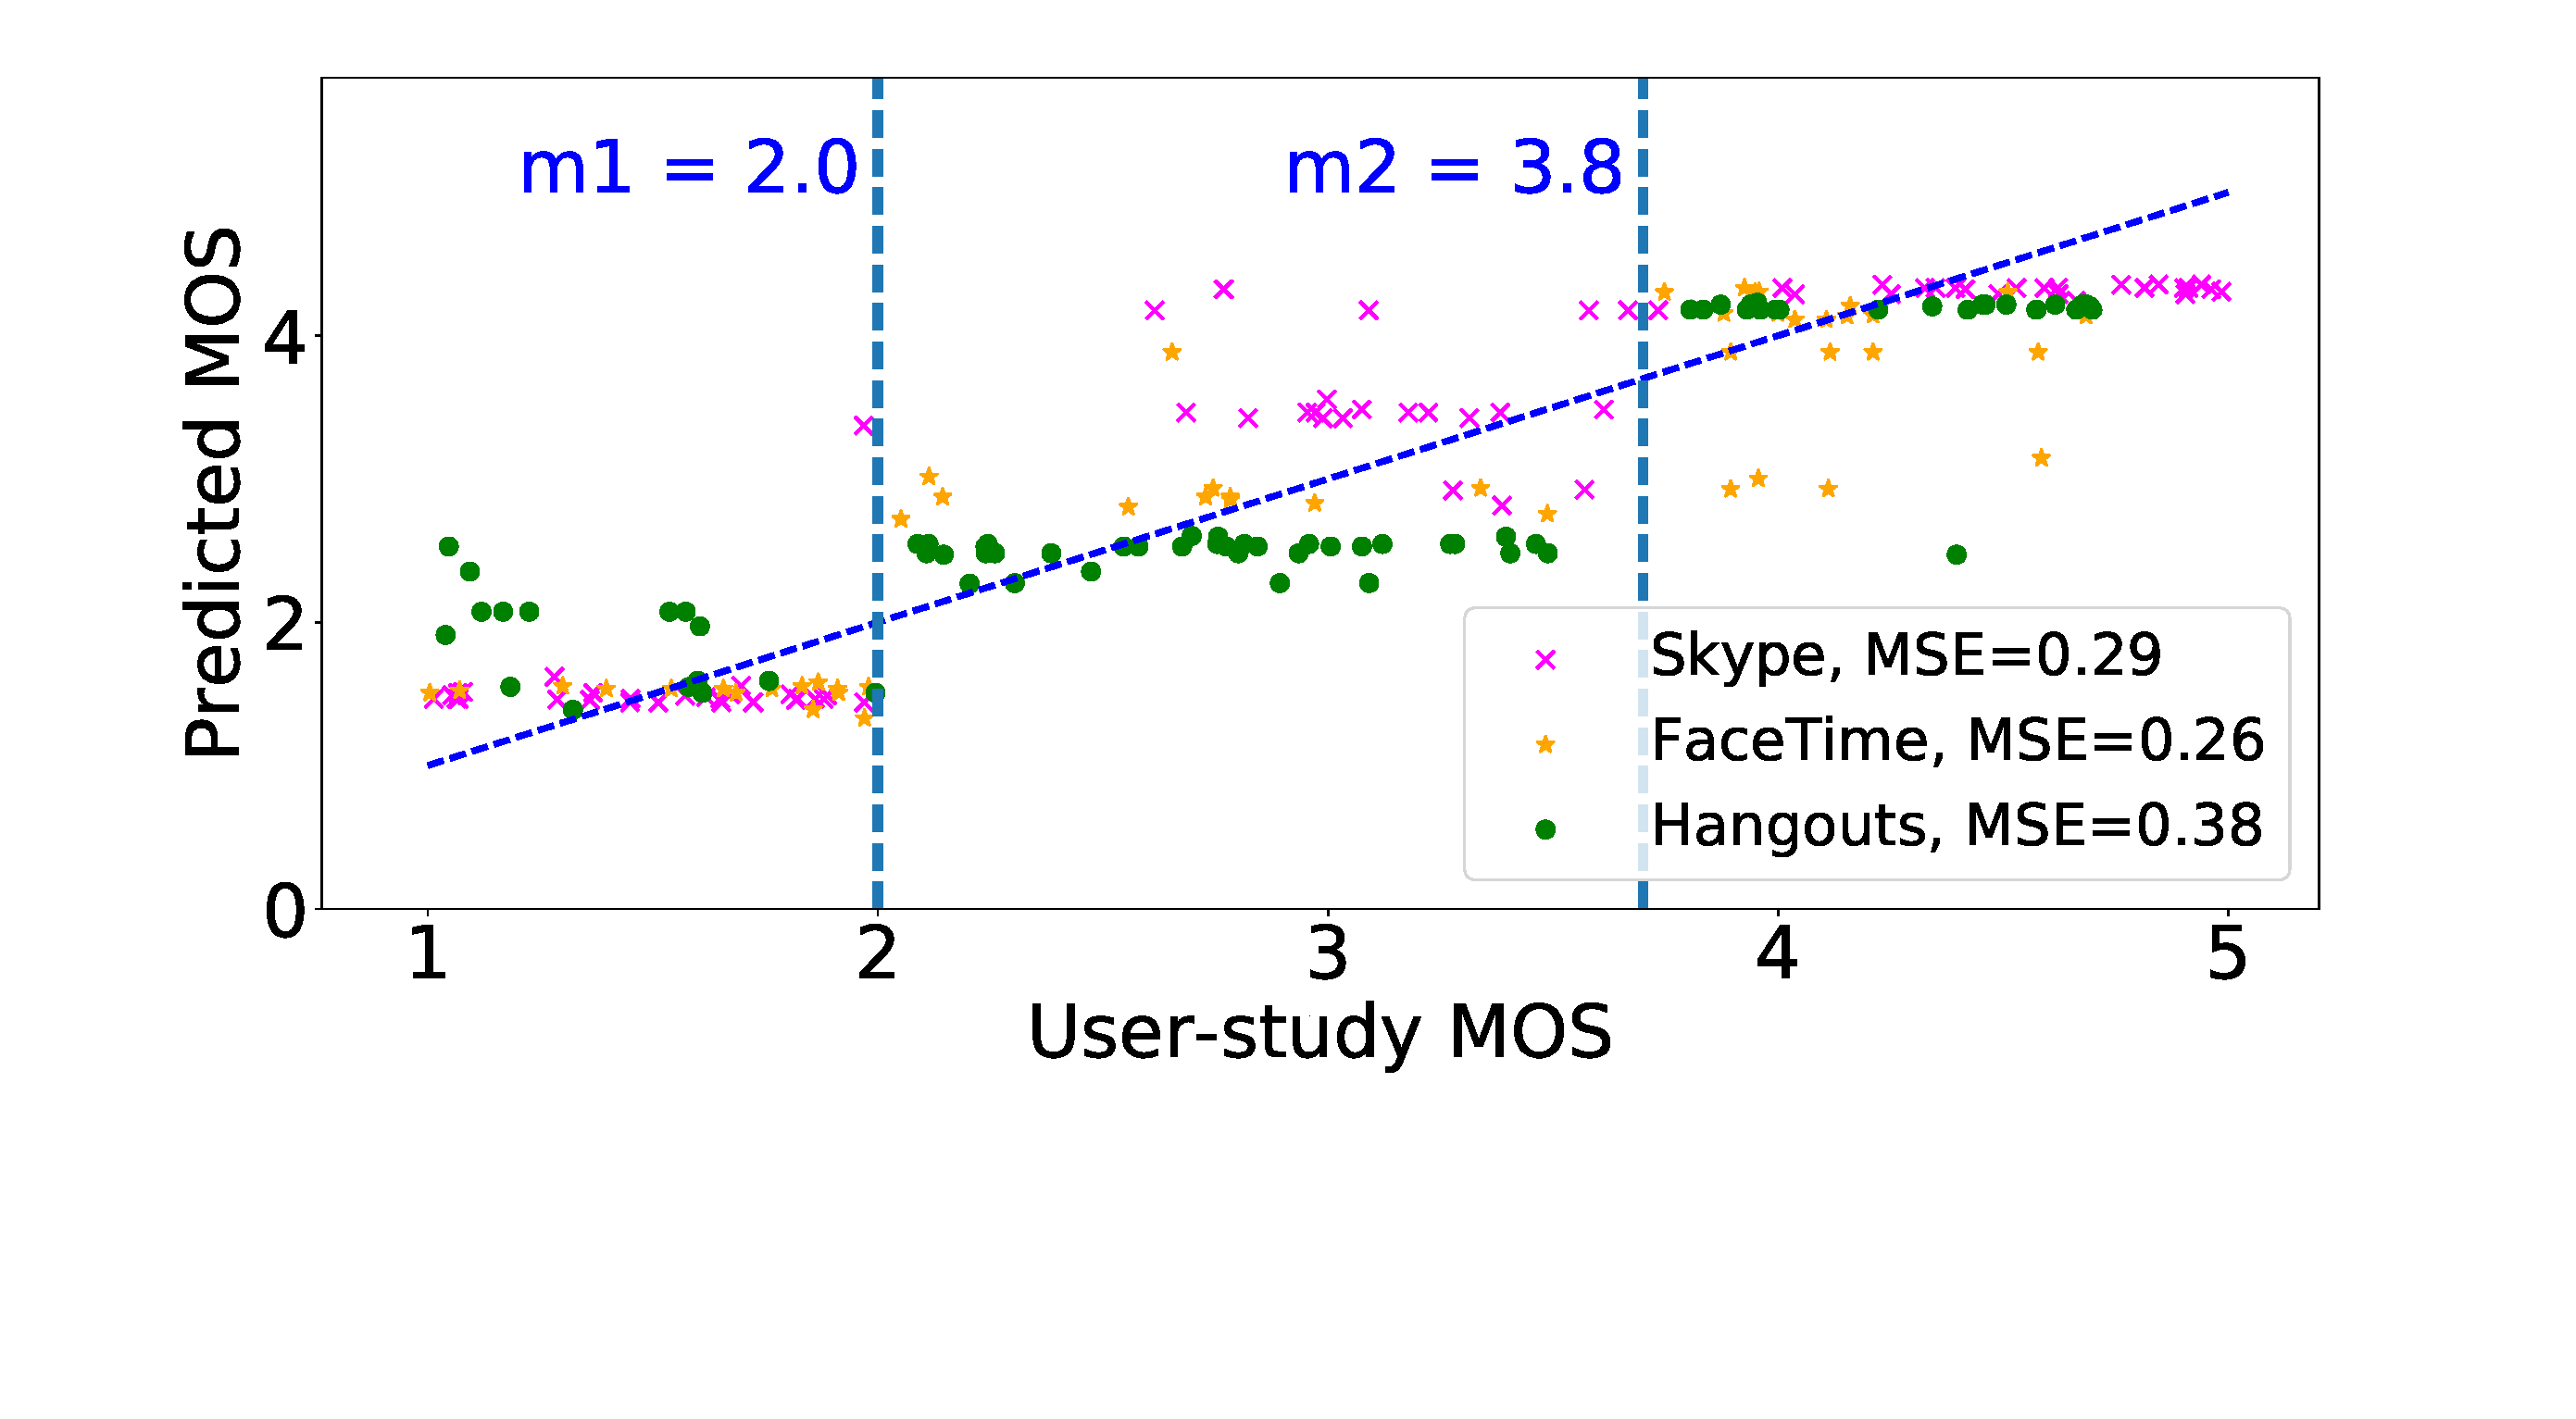
\includegraphics[width=\linewidth]{sections/network-work/scores.pdf}
      \vspace{-5em}
      \caption{User-study vs. predicted MOS for the three applications. We also show 3 clear QoE clusters divided by our thresholds $m_1=2$ and $m_2\approx 3.8.$}
      %\vspace{-1.7em}
      \label{fig:scores}
\end{figure}

Fig. \ref{fig:scores} shows a scatter plot of user-study MOS vs.~predicted MOS for the three applications. The MSE in MOS for the three applications is smaller than $0.4$ with ADT for all the applications. We also observe three clear clusters approximately divided by the MOS scores $m_1=2$ and $m_2=4$, that coincide with our thresholds for labeling the scores into 3 classes. This also justifies our design choice to finally employ three labels (bad, average, good) out of 5 MOS scores.

\noindent\textbf{Model performance for Skype:} 
Table \ref{class-skype} shows performance of Skype model across different regressors. 
The MSE in MOS is $0.29$ in case of ADT and it is $0.63$ with KNN regressor. 
Similarly, precision, accuracy and recall for ADT is the highest, while KNN being lowest.
ADT model gives a best threshold of $m_1=2$ and $m_2=3.8$ in separating the MOS scores into labels. While all the other models produce a threshold of $m_1=2$ and $m_2=3.4$.
Here, the best performance in ADT results from $(i)$ its low MSE and $(ii)$ the wide range for average class separation, i.e., it labels all the samples from MOS $2$ to $3.8$ as average class, while other models yield average class from MOS $2$ to $3.4$.
The performance gap is due to the distribution of our average class samples spread over wider range of bad or good labels. 
Using $m_1=2$ and $m_2=3.8$ thresholds, we get 30\%, 40\% and 30\% of our 300 samples in bad, average and good labels.

To show that our Skype model is device independent, we further evaluate our model across three devices: SG-S6 phone, SG-S2 Tab and Pixel Tab. Table \ref{label:skype-devices} shows precision, accuracy and recall for all three devices. We measure performance by training on one device, and testing on other devices. We observe that the performance is always better when trained and tested on the same device compared to training on one device and testing on other device. However, we find a difference of less than $7\%$ in accuracy when trained and tested across different devices, with an accuracy of at least 83\%. This corroborates that our model is robust across devices and it can be trained and tested without device constraints i.e., our metrics can collected on a certain device and can be applied to any other devices for Skype.

\noindent\textbf{Model performance for FaceTime:} 
Table \ref{class-facetime} shows performance of FaceTime model across different regressors.
Similar to Skype, we observe similar performance ($>89\%$ accuracy) for all models except the KNN regressor. 
Here, although the RF regressor is performing better ($90.37\%$ precision) than ADT, the MSE in MOS is larger than ADT.
Interestingly, all models produce same thresholds of $m_1=2$ and $m_2=3.4$ in labeling the scores.
Here, the samples are distributed uniformly across three classes unlike Skype, hence all regressors are performing almost equally. However, KNN regressor still suffers in FaceTime model due to weakness with many features as explained above. 
Using these thresholds, we get 30\%, 36\% and 34\% of the 200 samples in bad, average and good labels.

To validate that our FaceTime model is device independent, we train and test across iPad and iPhone devices.
Table \ref{label:facetime-devices} shows that when training and testing on same device, we observe $92\%$ accuracy. Whereas, training  and testing across devices yields at least $88\%$ accuracy. Hence, we observe a difference of $4\%$ accuracy across device training and testing. Our FaceTime model is also device-independent. Note that, we are not comparing the performance of our model training on Android devices and testing on iOS devices and vice-versa, because the recording set-up is different these environments.

\noindent\textbf{Model performance for Hangouts:} 
Table \ref{class-hangouts} shows performance of Hangouts model across different regressors.
Similar to other applications, ADT outperforms other models with 93.33\% accuracy with an average MSE of 0.38.
Similar to FaceTime, we observe that all models produce same thresholds of $m_1=2$ and $m_2=3.5$ in labeling the scores.
Using the above thresholds, we get 32\%, 34\% and 34\% of the 300 samples in bad, average and good labels respectively.

We further evaluate the Hangouts model across three devices: SG-S6 phone, SG-S2 Tab and Pixel Tab.
Table \ref{label:hangouts-devices} shows that an accuracy of at least 86.67\% when training and testing on same device, while inter-device train and test gives an accuracy of at least 82\%.
Overall, we observe less than 8\% accuracy difference when trained and tested across different devices. This shows that the model is independent of where training and tested are conducted.

\begin{figure}[t]
      \centering
      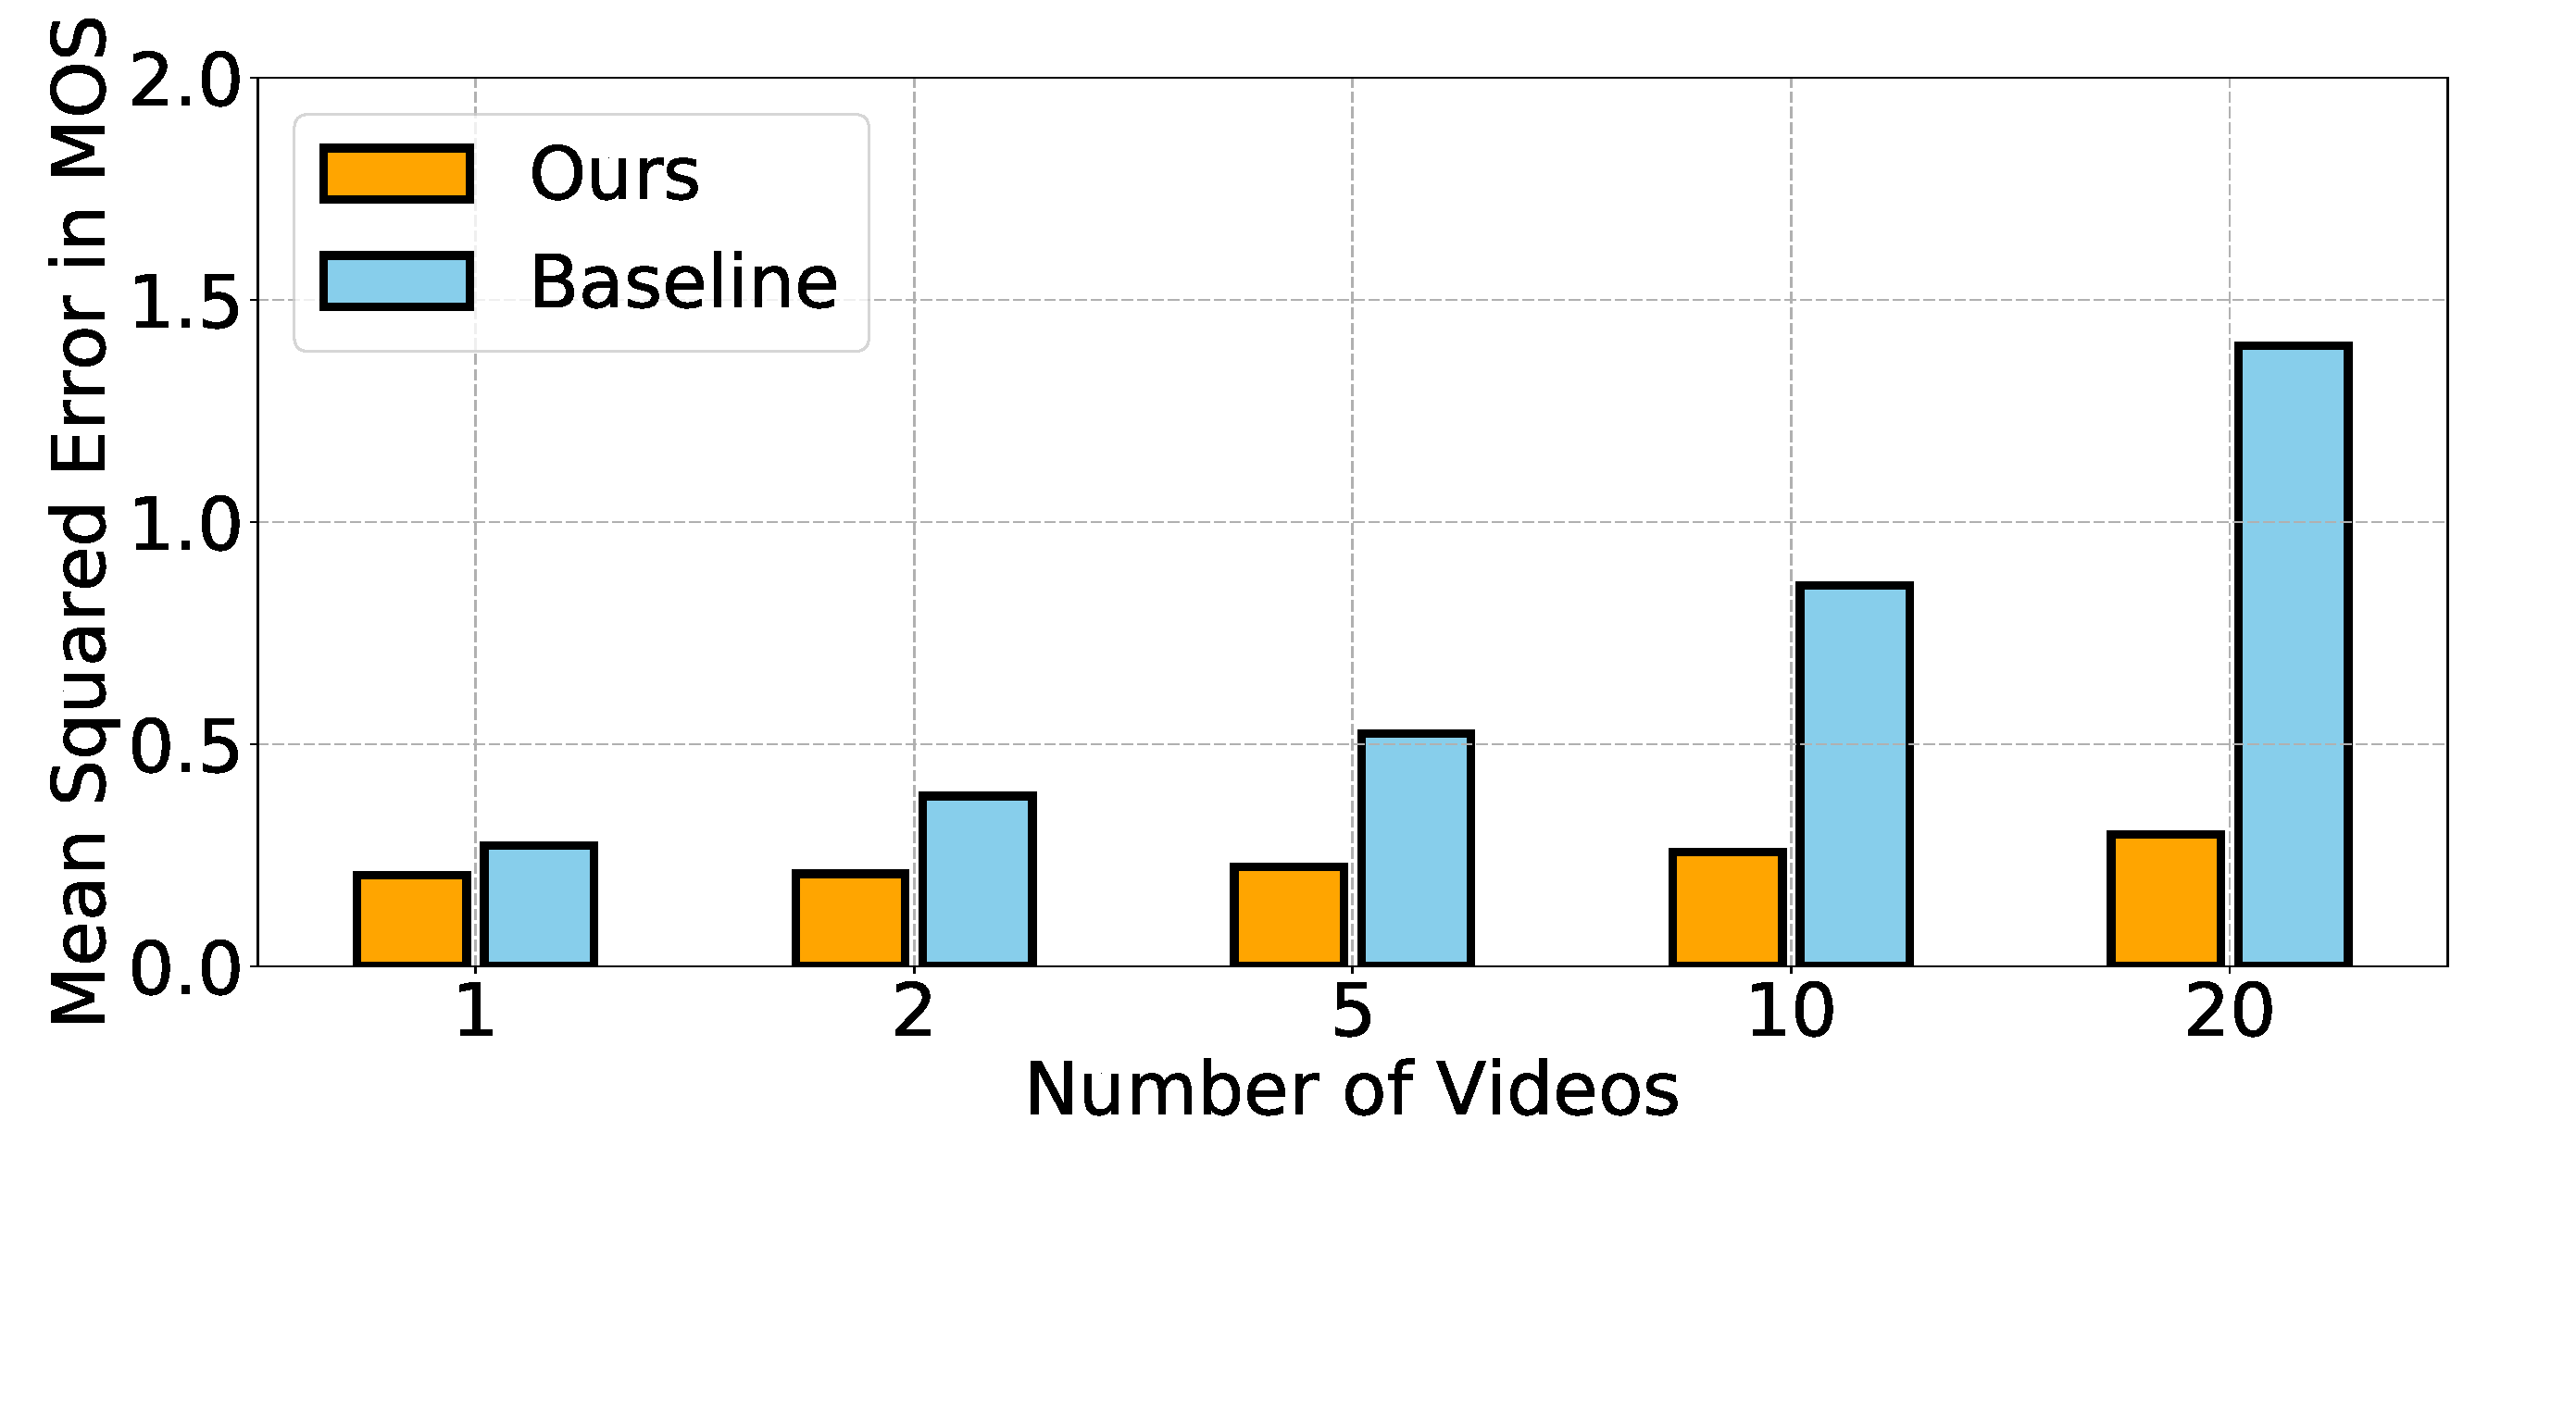
\includegraphics[width=\linewidth]{sections/network-work/baseline}
      \vspace{-3em}
      \caption{Comparison of our metrics vs.~baseline. Baseline has an up to 1.4 MOS estimation error across 20 video contents, hence failing to distinguish good/bad from average QoE. }
      %\vspace{-1.4em}
      \label{fig:baseline}
\end{figure}

\begin{figure}[t]
      \centering
      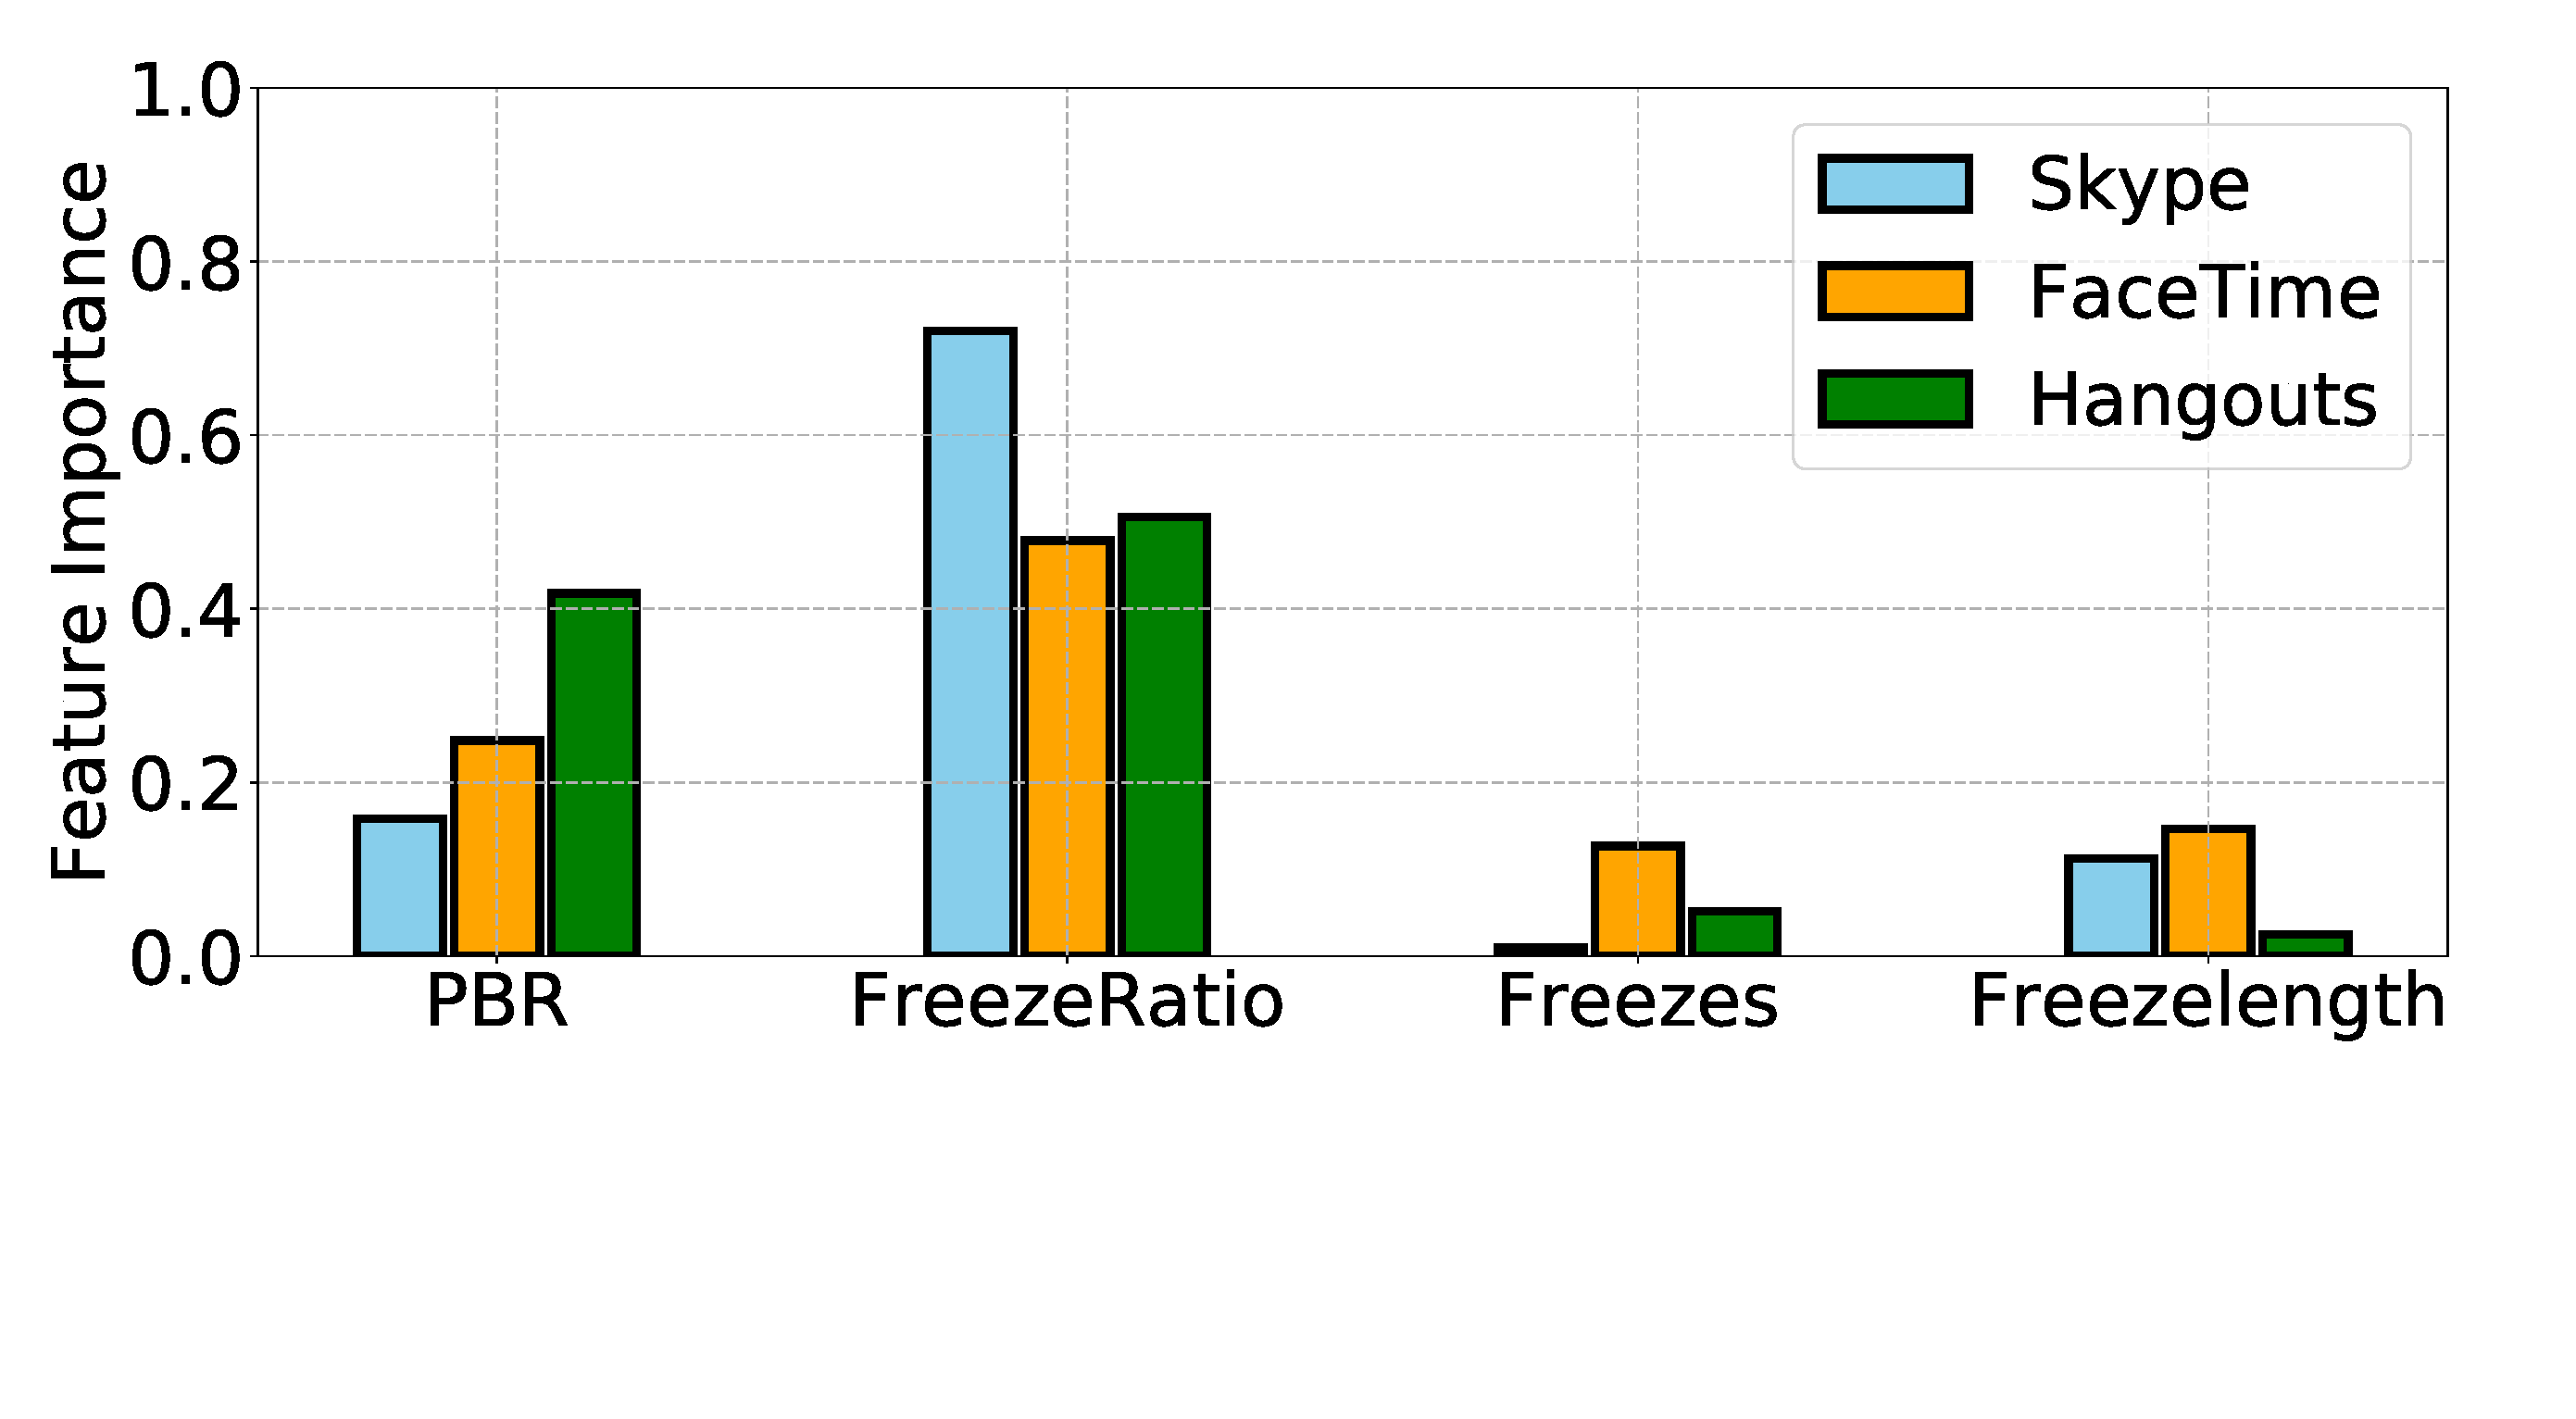
\includegraphics[width=\linewidth]{sections/network-work/feature-imp.pdf}
      \vspace{-4em}
      \caption{Feature Importance for the three applications.}
      %\vspace{-1.0em}
      \label{fig:ft-imp}
\end{figure}

\subsection{Comparison with Baseline and Feature Importance}
We compare our model prediction error with previous work for Skype application. As we need no-reference metrics for the baseline comparison, we use the DCT blur metric used by Jana {\em et al} as spatial metric and frame-drop metric in \cite{usman2017no} as temporal metric. We fit the ADT model with these two metrics as well as with our metrics using the MOS scores from our user-study. Fig. \ref{fig:baseline} shows the performance of Skype application across the 20 videos described in Section \ref{MOTIVATION}. Clearly, for a single video, both baseline and our model yield less than 0.2 MSE in MOS whereas as the number of videos increases, the MSE grows larger than 1.3 MOS for baseline metrics. Whereas, our model has a maximum of 0.4 MSE. The baseline metric's high MOS error with large number of videos is due to DCT metric's inability to scale across diverse video content. In fact, in our experiments we measure feature importance, which is defined as the amount each feature improves performance weighted by the number of samples this feature is responsible for. We observe that feature importance for DCT is as low as $0.1$, and it is $0.9$ for frame-drop metric. Therefore, previous metrics fail to model video telephony QoE across diverse videos. We observe similar results for FaceTime and Hangouts.

We also evaluate the importance of each proposed metric. Fig. \ref{fig:ft-imp} shows the importance of features for ADT over all three applications. Out of all features, freeze ratio is dominating with at least $0.5$ feature importance on all applications. For Skype, we observe highest ($>0.7$) importance to freeze ratio. The rest of the metrics are almost equally important, and removal of any of these features causes an up to 0.2 accuracy degradation. Whereas, for FaceTime and Hangouts, we notice high importance for PBR ($0.28$ for FaceTime and $0.41$ for Hangouts) due to their compromise in quality over freezes.


\section{Related Works}
\subsection{Network-specific Optimizations}
There is an extensive prior work on video QoE modeling. The vast majority of works \cite{aggarwal2014prometheus,balachandran2013developing,fiedler2010generic} introduce machine learning methods to map QoS to QoE, and assume availability of the QoE ground-truth. Features for QoE estimation can be collected from various vantage points, such as on the application server~\cite{balachandran2013developing}, on the end-device (application-client statistics or packet capturing)~\cite{zhang2012profiling,yu2014can,seufert2015survey,aggarwal2014prometheus,balachandran2012quest,chen2014qoe}, or the access network (e.g., WiFi AP or LTE base station)~\cite{chakraborty2016exbox,jana2016qoe,chen2006quantifying}. Compared to the above works, we focus on annotating QoE ground-truth, hence easing the extension of QoS to QoE mappings to all video-telephony applications. Our work significantly advances state-of-the-art QoE labeling at the training phase of QoS to QoE, by introducing accurate metrics that capture spatial and temporal video quality.

\noindent
\textbf{Spatial quality assessment:}  Prior works have proposed multiple metrics to capture video blurriness (spatial artefacts). Jana et al.~\cite{jana2016qoe} introduce metrics for freezes, blocking and blur over Skype and Vtok. However, as we show in Section~\ref{MOTIVATION}, this blur metric is highly content dependent. We have found similar results for major prior works~\cite{golestaneh2014no, mittal2012no,tong2004blur,marziliano2002no} on no-reference blur detection. In Section V, we present more than 1 MOS lower estimation error for our metrics compared to prior work over 20 diverse videos. We have not observed blocking artefacts in any of Skype, FaceTime or Hangouts applications.

\noindent
\textbf{Temporal quality assessment:} Several works \cite{wolf2009no, borer2010model, usman2017no, pastrana2006automatic} have investigated the effect of video freezes on user QoE. Wolf and Pinson~\cite{wolf2009no} propose to use the motion energy temporal history of videos, along with framerate of video. This requires additional information from original video hence, making it a reduced reference metric. Similarly, the temporal metric of Jana et al.~\cite{jana2016qoe} is a reduced-reference metric. The temporal metric by Pastrana-Vidal and Gicquel~\cite{pastrana2006automatic} is sensitive to resolution and content of the video. Different from all of these works, we present three content-independent, no-reference temporal metrics to assess temporal video artefacts.

\noindent \textbf{Machine learning based quality assessment:} There has been a lot work in the space of image quality assessment using machine learning \cite{hou2015blind}\cite{ye2012unsupervised} and recently deep learning \cite{mocanu2014deep}\cite{xue2013learning}\cite{narwaria2010objective}. A relatively few works have focused on video quality assessment \cite{le2006convolutional}\cite{narwaria2012low}. However, most of these models limited either spatial or temporal feature extraction. Moreover, the datasets used these models are not enough to evaluate the scalability of the models. In our model, we carefully select 20 different video as described in \S \ref{MOTIVATION} and apply both spatio-temporal feature extraction methods.

\section{Conclusion}
Enterprise network administrators need QoE information to model QoS to QoE relationship and to efficiently provision their resources. Currently, applications do not provide QoE ground-truth. In this work, we address this problem for video telephony by introducing four scalable, no-reference QoE metrics that capture spatial and temporal artefacts of video quality. We investigate the performance of our metrics over three popular applications -- Skype, FaceTime and Hangouts -- across diverse video content and five mobile devices. Finally, we map our metrics with a large-scale MOS user-study and show a median accuracy of 90\% in annotating the QoE labels according to MOS. Our metrics outperform state-of-the-art work while capturing exact user rating. We plan to extend this study to video streaming, such as YouTube and Netflix, and VR/AR applications.

\bibliographystyle{plain}
\bibliography{qos-qoe}
\end{document}
